\documentclass{pnp_article}

\begin{document}

\SetDocIssue{1.0}
\SetDocRefNumber{PP-UM-COR-0002}
\SetDocTitle{The CORDET Framework}
\SetDocSubtitle{User Manual}
\SetDocAuthor{Alessandro Pasetti}
\SetCheckedBy{n.a.}
\maketitle

% =======================================================================
%\listofchanges
\tableofcontents
\listoffigures
\listoftables

%---------------------------------------------
% Start of document text
%---------------------------------------------
\section{Referenced Documents}

The documents referenced in the present document are listed in the table below.

\listofreferencedocs{\CrUm}




%==========================================================================================
\newpage
\section{Introduction}
This document is the User Manual for the \textit{C2 Implementation}. 
The C2 Implementation is a C-language implementation of the \textit{CORDET Framework}.
The CORDET Framework is a software framework for service-oriented applications. 

The CORDET Framework defines an application in terms of the services it provides to other applications and in terms of the services it uses from other applications.
A \textit{service} is implemented by a set of \textit{commands} through which an application is asked to perform certain activities and by a set of \textit{reports} through which an application gives visibility over its internal state.

A service is implemented by a set of commands through which an application is asked to perform certain activities and by a set of reports through which an application gives visibility over its internal state. The CORDET Framework defines the components to receive, send, distribute, and process commands and reports (the \textit{CORDET Components}).

The CORDET service concepts supports the implementation of distributed systems of applications where individual applications residing on different distribution nodes interact through the exchange of commands and reports.

The CORDET Framework is specified in reference [CR-SP]. This specification is implementation-independent. The C2 Implementation is an implementation of the CORDET Components in the ANSI C language.

The main features of the C2 Implementation are:
\begin{fw_itemize}
\item{} \textbf{Well-{}Defined Semantics}: clearly and unambiguously defined behaviour.
\item{} \textbf{Minimal Memory and CPU Requirements}: core module footprint of less than 20 kBytes and efficient implementation in C.
\item{} \textbf{Scalability}: code memory footprint independent of the number of commands and reports.
\item{} \textbf{High Reliability}: test suite with 100\% code, branch, and condition coverage.
\item{} \textbf{Formal Specification}: user requirements to formally specify the implementation.
\item{} \textbf{Requirement Traceability}: all requirements individually traced to their implementation and to verification evidence.
\item{} \textbf{Documented Code}: doxygen documentation for all the source code.
\item \textbf{Demo Applications}: complete applications demonstrating capabilities and mode of use.
\end{fw_itemize}



The behaviour of the CORDET components is modelled by means of state machines and procedures (activitiy diagrams). The semantics of the state machines and procedure is the one defined by the FW Profile of reference [FW-SP]. The C2 Implementation of the CORDET Framework implements these state machines and procedures using a C-language implementation of the FW Profile \footnote{The implementation of the FW Profile state machines and procedure is also available as a separate and self-contained delivery under the name of C1 Implementation, see reference [FW-SP]}. 

%------------------------------------------------------------------------------------------
\section{Installation \& Content Overview}\label{sec:InstAndContentOverview}
The C2 Implementation is delivered as one single zip file (the \emph{delivery file}).
This file should be expanded in a dedicated directory. 
This directory becomes the \emph{host directory} for the C2 Implementation.
Table \ref{tab:HostDir} gives an overview of the structure of the host directory.
More details are found in subsequent subsections.

The C2 Implementation software is delivered as source code and therefore no further installation operations are needed. A Test Suite is provided together with Unix script files to compile and link it.

\begin{longtable}{|l|p{11cm}|}
\caption{Structure of Host Directory}\label{tab:HostDir} \\
\hline
\rowcolor{light-gray}
\textbf{Sub-Dir.} & \textbf{Sub-Directory Description}\\
\hline\hline
\texttt{/docs} & Support documentation for C2 Implementation. See section \ref{sec:SupportDoc}.\\
\hline
\texttt{/lib} & Framework Profile source code. See section \ref{sec:depC1}.\\
\hline
\texttt{/log} & Test reports generated by Acceptance Test Procedure. See section \ref{sec:atp}.\\
\hline
\texttt{/src} & Source code for the CORDET Framework. See section \ref{sec:fwSrcCode}.\\
\hline
\texttt{/tests} & Source code for the Test Suite. See section \ref{sec:fwSrcCode}.\\
\hline
\end{longtable}

%--------------------------------------------------------------------------------------------
\subsection{Dependency on C1 Implementation}\label{sec:depC1}
The behaviour of the CORDET Framework is specified by means of state machines and procedures (activity diagrams). The implementation of the framework therefore requires an implementation of state machines and procedures. The C2 Implementation does not include an own implementation of state machines and procedures. Instead, it uses the state machine and procedure modules of the C1 Implementation of the FW Profile (see reference [FW-SP]). These modules can be downloaded from: \texttt{http://pnp-software.com/fwprofile} but, for convenience, they are also included in the C2 Implementation Delivery File.

Note that the C1 Implementation consists of three modules covering the implementation of, respectively, state machines, procedures and RT Containers (encapsulations of threads). The third module is not used by the CORDET Framework.

%--------------------------------------------------------------------------------------------
\subsection{Dependency on External Libraries}
The C2 Implementation (namely the CORDET Components in directory \texttt{/src}) only needs the \texttt{stdlib} and the \texttt{string} libraries of the C language and the State Machine and Procedure Modules of the C1 Implementation of the FW Profile. The C1 Implementation modules are delivered together with the C2 Implementation (see previous section). 

The Test Suite (namely the modules in directory \texttt{/tests}) use additional libraries and POSIX services. In particular, the shell scripts which are delivered with the C2 Implementation (see section \ref{sec:script}) to generate the executable for the Test Suite need an implementation of the POSIX library. The scripts link the POSIX library with option \texttt{-lpthread}. Users with different implementations of the POSIX library will have to modify the scripts accordingly. Users without a POSIX library implementation will not be able to build the Test Suite (but will, of course, still be able to use the CORDET Components in their own applications).

%--------------------------------------------------------------------------------------------
\subsection{Source Code}\label{sec:fwSrcCode}

The source code in the CORDET delivery file covers one instantiation of the CORDET Framework for the \textit{Test Suite} (see section \ref{sec:TestSuite}). 

At source code level, an instantiation of the CORDET Framework to implement an application within the framework's domain can be split into four parts:

\begin{itemize}
\item \textit{Invariant Framework Software} consisting of the implementation of the CORDET Components. This part is common to all instantiations of the CORDET Framework. 
\item \textit{Configurable Framework Software} consisting of the part of the framework which must be modified to be adapted to the needs of each end-application (the adaptation model for the framework is described in section \ref{sec:AdaptationModel}). This part is customized for each instantiations of the CORDET Framework. 
\item \textit{C1 Implementation Software} providing an implementation of the state machine and procedure (activity diagram) concepts (see section \ref{sec:depC1}). This part is common to all instantiations of the CORDET Framework.
\item \textit{Application-Specific Software} implementing the application-specific (i.e. non-framework) part of the target application. 
\end{itemize}

The souce code in the CORDET delivery file is accordingly split into several directories as presented in table \ref{tab:srcCrDeliveryFile}. Users who wish to build a new application by instantiating the CORDET Framework would normally take the software in directories \texttt{/src} and \texttt{/lib/fwprofile/src} without changes and would customize the software in one of the \texttt{Config} directories to match their needs. The instantiation process is described in greater detail in section \ref{sec:FwInstantiation}.

\begin{longtable}{|l|p{9cm}|}
\caption{Source Code in CORDET Delivery File}\label{tab:srcCrDeliveryFile} \\
\hline
\rowcolor{light-gray}
\textbf{Sub-Directory} & \textbf{Sub-Directory Description}\\
\endfirsthead
\rowcolor{light-gray}
\textbf{Sub-Directory} & \textbf{Sub-Directory Description}\\
\hline\hline
\endhead

\texttt{/src} & Invariant Framework Software implementin the CORDET Components. For each CORDET Component, a dedicated sub-directory is present which holds the code implementing the component. The name of the sub-directory is the same as the name of the component. The code in this directory is used unchanged in all applications instantiated from the CORDET Framework. \\
\hline
\texttt{/lib/fwprofile/src} & Source code for the State Machine and Procedure modules of the C1 Implementation of the FW Profile. The code in this directory is used unchanged in all applications instantiated from the CORDET Framework. \\
\hline
\texttt{/tests} & Application-Specific Software for the Test Suite application. \\
\hline
\texttt{/tests/config} & Configurable Framework Software for the Test Suite application. \\
\hline
\end{longtable}


%------------------------------------------------------------------------------------
\newpage
\subsection{Support Documentation}\label{sec:SupportDoc}
The C2 Implementation is delivered with the following support documents: 

\begin{itemize}
\item The \textbf{CORDET Framework Definition Document} which specifies the framework implemented by the C2 Implementation
\item A \textbf{User Manual} (this document) which describes how the C2 Implementation is used
\item A \textbf{User Requirement Document} which formally specifies the C2 Implementation
through a set of requirements and provides validation and verification evidence for each requirement
\end{itemize}

These documents, together with the Test Suite and the detailed software documentation in the Doxygen web site, constitute the \textbf{Qualification Data Package} (QDP) for the C2 Implementation. The QDP is provided for users who need to certify their application or, more generally, who need to provide evidence of its correctness. The QDP contains the typical information which is required for software certification purposes. It can therefore be included in the certification data package of end-applications and it relieves the user of the need to produce such information for the C2 Implementation part of their applications.

%------------------------------------------------------------------------------------
\subsection{Doxygen Documentation}\label{sec:DoxygenDoc}
All the source code in the C2 Implementation (including the test suite) is documented in accordance with doxygen rules. The entry point to the Doxygen documentation is the \texttt{index.html} file in the \texttt{/docs/doxygen} directory.

%------------------------------------------------------------------------------------
\subsection{Test Suite}\label{sec:TestSuite}
The Test Suite is a complete application which demonstrates all aspects of the behaviour of the CORDET Components.

The main program of the Test Suite application is in file \texttt{CrTestSuite.c}. This program consists of a set of test cases. For each CORDET Component, one or more test cases are defined. Each test case exercises a specific aspect of the behaviour of a CORDET Component. The Test Suite offers 100\% code, branch, and condition coverage of the CORDET Components.

On a Unix platform, the Test Suite application can be built by running one of the support scripts delivered with the C2 Implementation (see section \ref{sec:script}). 

%----------------------------------------------------------------------------------------------
\subsection{Acceptance Test Procedure and Test Reports}\label{sec:atp}
The C2 Implementation is passed through an Acceptance Test Procedure (ATP) prior to its release. The ATP is executed as a sequence of steps which are defined in table \ref{tab:atp}. For each step, a pass-fail criterium is defined. An execution of the ATP is successful if all the ATP steps satisfy their pass-fail criteria.

\newpage
\begin{longtable}{|l|p{6.2cm}|p{6.2cm}|}
\caption{Execution Steps and Pass-Fail Criteria for ATP}\label{tab:atp} \\
\hline
\rowcolor{light-gray}
\textbf{N} & \textbf{Step} & \textbf{Pass-Fail Criterium} \\
\hline\hline
\endfirsthead
\rowcolor{light-gray}
\textbf{N} & \textbf{Step} & \textbf{Pass-Fail Criterium} \\
\hline\hline
\endhead

1 & Run Doxygen using Doxygen Configuration File on the entire source code of the C2 Implementation delivery &
Neither errors nor warnings are reported by Doxygen \\
\hline
2 & Compile the C2 Implementation source code with "all warnings" enabled and with the options required to run GCov for both branch and statement coverage &
Neither errors nor warnings are reported by the compiler \\
\hline
3 & Compile the Test Suite source code files with "all warnings" enabled &
Neither errors nor warnings are reported by the compiler \\
\hline
4 & Build the executable to run the Test Suite for the C2 Implementation and to generate the \texttt{*.gcno} and \texttt{*.gcda} files &
Neither errors nor warnings are reported by the linker \\
\hline
5 & Run the Test Suite with Valgrind &
The Test Suite runs to completion; all test cases are declared to have completed successfully; no errors are reported by Valgrind in addition to, possibly, the errors discussed below \\
\hline
6 & Run GCov on all the C2 Implementation Files to which coverage requirements apply &
For each C2 Implementation File to which coverage requirements apply, a \texttt{*.c.gcov}
file is created and the file shows full statement and branch coverage with exception of
branches entered as a result of a failure of \texttt{malloc} \\
\hline
\end{longtable}

With reference to point 5, it is noted that, on many platforms, Valgrind will report 3 possible memory leaks originating in function \texttt{pthread\_create}. This is a known issue in many POSIX libraries and is not related to the CORDET Framework code.

The \texttt{RunAcceptanceTest.sh} shell script (not included in the delivery for end customers) automatically executes all the procedure steps described in the table and it generates a test report which is included in directory \texttt{\\reports} of the delivery file.

%------------------------------------------------------------------------------------
\subsection{Support Scripts}\label{sec:script}
To build the Test Suite a Makefile is provided in the root directory. This Makefile can be used with the generally available \texttt{make} tool to generate different targets. The following targets are supported:

\begin{itemize}
\item \texttt{make test} Generates the test suite
\item \texttt{make run-test} Runs the test suite
\item \texttt{make coverage-info} Generates the gcov files which contain the coverage information
\end{itemize}

The test suite is created in the \texttt{/bin} sub-directory.


%------------------------------------------------------------------------------------
\subsection{Naming Conventions}
The C2 Implementation exports the following items towards users:

\begin{itemize}
\item Header and body files
\item Global functions
\item Types defined through \texttt{typedef} 
\item Constants and macros defined through \texttt{\#define} directives
\end{itemize}

The naming conventions for these items are as follows.
 
The names of the header and body files of the C2 Implementation and of the global 
functions they export are written as a concatenation of strings (without underscores). 
The first letter in each string is capitalized. The names have the following form: 
\texttt{Cr<Xx><Name>}. The prefix "\texttt{Cr}" identifies a name as belonging to the CORDET Framework implementation. 
The string "\texttt{Xx}" identifies the domain within the CORDET world 
to which the name belongs. The following values are possible for this string: 

\begin{itemize}
\item "\texttt{Fw}" identifies a name related to the implementation of the CORDET Framework and of its Test Suite, 
\end{itemize}

The string "\texttt{Name}" is the proper name of the function or file and it is made up of a concatenation of other strings. The following abbreviations are used in forming this name:

\begin{itemize}
\item "\texttt{A}": "\texttt{action}" (as in "action node")
\item "\texttt{Act}": "\texttt{action}" (as in "action attached to a procedure node")
\item "\texttt{App}": "\texttt{application}" (as in "the Demo Application")
\item "\texttt{Aux}": "\texttt{auxiliary}" (as in "auxiliary function")
\item "\texttt{Config}": "\texttt{configuration}" (as in "the configuration of a component")
\item "\texttt{Cmd}": "\texttt{command}"
\item "\texttt{Cmp}": "\texttt{component}"
\item "\texttt{Cnt}": "\texttt{counter}"
\item "\texttt{Cps}": "\texttt{choice pseudo-state}"
\item "\texttt{Cr}": "\texttt{CORDET}" 
\item "\texttt{Cre}": "\texttt{creation}" 
\item "\texttt{Cur}": "\texttt{current}" (as in "current state of a state machine")
\item "\texttt{D}": "\texttt{decision}" (as in "decision node")
\item "\texttt{Dec}": "\texttt{decision}" (as in "decision node in a procedure")
\item "\texttt{Der}": "\texttt{derived}" (as in "the derived state machine")
\item "\texttt{Desc}": "\texttt{descriptor}" (as in "the descriptor of a state machine")
\item "\texttt{Fin}": "\texttt{final}" (as in "final node")
\item "\texttt{Fw}": "\texttt{framework}" 
\item "\texttt{Err}": "\texttt{error}" (as in "the application error code")
\item "\texttt{Emb}": "\texttt{embedded}" (as in "embedded state machine")
\item "\texttt{Fps}": "\texttt{final pseudo-state}"
\item "\texttt{Ini}": "\texttt{initial}" (as in "initial mode")
\item "\texttt{Init}": "\texttt{initialization}" (as in "initialization of a component")
\item "\texttt{Ips}": "\texttt{initial pseudo-state}"
\item "\texttt{Pckt}": "\texttt{packet}" (as in "the command is encapsulated in a packet")
\item "\texttt{Pr}": "\texttt{procedure}"
\item "\texttt{Rec}": "\texttt{recursive}" (as in "recursive function")
\item "\texttt{Rep}": "\texttt{report}"
\item "\texttt{Sm}": "\texttt{state machine}"
\item "\texttt{Sta}": "\texttt{state}" (as in "the state of a state machine")
\item "\texttt{Temp}": "\texttt{temperature}"
\item "\texttt{Trans}": "\texttt{transition}" (as in "the transition between two states")
\end{itemize}

The names of the types defined through \texttt{typedef} start with the string "\texttt{CrFw}" and 
terminate with the string: "\texttt{\_t}".

The names of the \texttt{\#define} constants are written in capitals and are made 
up of strings concatenated with underscores.

%---------------------------------------------------------------------------------
\section{Framework and Service Concepts}
The CORDET Framework is a software framework to support the instantiation of service-oriented applications. 
This section gives an overview of the software framework concept and of the service concept assumed in the CORDET project.
A fuller version of the material presented in this section can be found in reference [CR-SP].

%----------------------------------------------------------------------------------------
\subsection{Software Framework Concept}\label{sec:SwFwConcept} 
A software framework is a repository of reusable and adaptable software components embedded within a pre-defined architecture that is optimized for applications in a certain domain (see figure \ref{fig:SwFwConcept}).

\begin{figure}[ht]
 \centering
 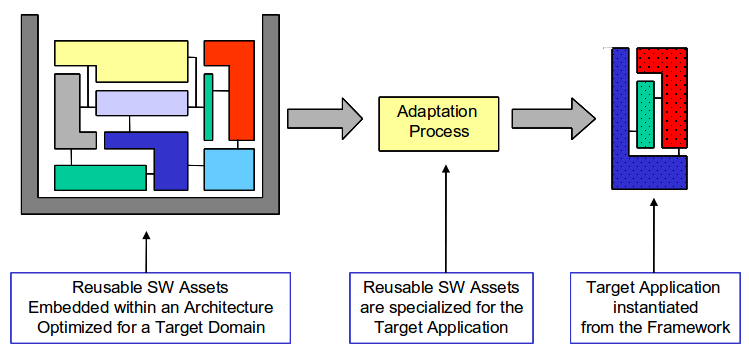
\includegraphics[scale=0.5,keepaspectratio=true]{SwFwConcept.png}
 \caption{Software Framework Concept}
 \label{fig:SwFwConcept}
\end{figure}

The framework components are reusable in the sense that they encapsulate behaviour which is common to all (or at least a large number of) applications within the framework's domain.

To reuse a software components means to use it in different operational contexts. 
In practice, varying operational contexts always impose different requirements. 
Hence, reuse requires that the reusable components be \textit{adaptable} to different requirements. 
In this sense, adaptability is the key to reusability. 
For this reason, framework components offer \textit{adaptation points} where their behaviour can be modified to match the needs of specific applications.

Framework components are embedded within a pre-defined architecture in the sense that the framework does not simply specify individual components but it also specifies their mutual relationships. 
Thus, the unit of reuse of a software framework is not a component but rather a group of cooperating components which, taken together, support the implementation of some functionality that is important within the framework domain. 

Software frameworks encourage this higher granularity of reuse by being organized as a bundle of functionalities that users can choose to include in their applications. 
Inclusion of a functionality implies that a whole set of cooperating components and interfaces is imported into the application. 

In the service-oriented concept underlying the CORDET Framework, the functionalities supported by the framework are the “services” as defined in the next section.

The \textit{domain} of a framework is the set of applications whose instantiation is supported by the framework. The domain of the CORDET Framework are the applications which comply with the CORDET service Concept introduced in section \ref{sec:ServConcept}.



%----------------------------------------------------------------------------------------
\subsection{Service Concept}\label{sec:ServConcept} 
The target domain of the CORDET Framework are service-oriented applications. 
This section defines the service concept assumed in the CORDET Project (the \textit{CORDET Service Concept}).

A \textit{service} is a set of logically and functionally related capabilities that an application offers to other applications. 
The CORDET Service concept sees an application as a \textit{provider of services} to other applications and as a \textit{user of services} from other applications (see figure \ref{fig:ServConcept}).

A service is identified by its \textit{type}. 
The service type is a positive integer which uniquely identifies the service within the CORDET world and thus acts as a name for the service.

\begin{figure}[ht]
 \centering
 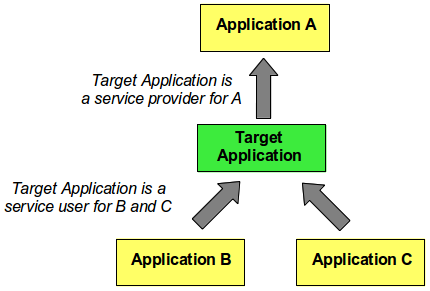
\includegraphics[scale=0.55,keepaspectratio=true]{ServConcept.png}
 \caption{Applications as Providers and Users of Services}
 \label{fig:ServConcept}
\end{figure}

The user of a service controls the service by sending \textit{commands} to the service provider. 
A command is a data exchange between a service user and a service provider to start, advance, modify, terminate, or otherwise control the execution of a particular activity within the service provider (see reference \cite{ref:pus}, section 3.1.13). 

The provider of a service sends \textit{reports} to the user of the service. 
A report is a data exchange between a service provider (the report initiator) and a service user to provide information relating to the execution of a service activity (see reference \cite{ref:pus}, section 3.1.14).

Thus, a service consists of a set of commands which the user of the service sends to the provider of the service and of a set of reports which the service provider sends back to its user. 
A command defines actions to be executed by the service provider. 
A report encapsulates information about the internal state of the service provider (see figure \ref{fig:ServCmdRep}).

\begin{figure}[ht]
 \centering
 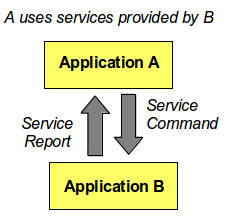
\includegraphics[scale=0.5,keepaspectratio=true]{ServCmdRep.png}
 \caption{Services as Sets of Commands and Reports}
 \label{fig:ServCmdRep}
\end{figure}

The same application may act as as a service provider to several user applications and, vice-versa, it may use the services from several other providers. For instance, in figure \ref{fig:ServConcept}, the Target Application has one user (Application A) and it acts as user for two service providers (Applications B and C). 

Figures \ref{fig:ServConcept} and \ref{fig:ServCmdRep} show situations where the service provider and service users have a direct connection but the CORDET Service Concept also supports situations where the connection between provider and user is indirect.

In figure \ref{fig:ServRerouting}, for instance, application A sends a command to application C but the command is routed through application B. 
Thus, the CORDET Service Concept can be used as a basis for the definition of distributed applications which interact with each other by exchanging service requests over a network. 

The network defines physical links between the applications in the system (e.g. the links between applications A and B and between applications B and C in figure \ref{fig:ServRerouting}) and the CORDET infrastructure defines logical links between the applications (e.g. the link between applications A and C).

\begin{figure}[ht]
 \centering
 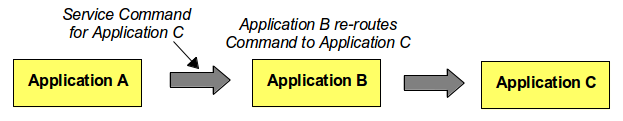
\includegraphics[scale=0.5,keepaspectratio=true]{ServRerouting.png}
 \caption{Re-Routing of Service Requests}
 \label{fig:ServRerouting}
\end{figure}



%----------------------------------------------------------------------------------------
\subsection{Objectives of CORDET Framework}\label{sec:ObjectivesOfCrFw} 

In general terms, the goal of the CORDET Framework is to foster software reusability in the development of service-oriented embedded control applications. 

With a service-oriented concept, an application is specified in terms of the services it offers to other applications and of the services it needs from other applications and the services are in turn specified by the commands and reports which implement them.

In this perspective, the CORDET Framework supports reusability in the following ways:

\begin{enumerate}
\item{} It provides a formal definition of the abstract (implementation-independent) concept of commands and reports,
\item{} It specifies the components (the CORDET Components) which implement the abstract command and report concepts and the CORDET Standard Services, and
\item{} It allows services of general applicability for a specific domain to be pre-defined and to be available as building blocks for the development of applications in that domain.
\end{enumerate}

Each of the above three points is discussed in greater detail in a dedicated sub-section below. 

%----------------------------------------------------------------------------------------
\subsubsection{Definition of Command and Report Concepts}\label{sec:DefCmdRepConcepts}

The first objective of the CORDET Framework is to provide a formal definition of the abstract command concept and of the abstract report concept. 

This is done by building behavioural models of commands and of reports which:

\begin{enumerate}
\item{} capture the aspects of the behaviour of commands and reports which is common to all commands and reports independently of the definition and implementation of a concrete command or report, and
\item{} identify the adaptation points where service- and implementation-specific behaviour can be added.
\end{enumerate}

An example may clarify the definition given above. 
In section \ref{sec:CmdCondChecks}, the concept of Acceptance Check for commands is introduced. 
An acceptance check is a check that is performed upon incoming commands to determine whether the command can be accepted or whether it should be rejected. 
The abstract concept of command includes the following behavioural property: “an incoming command shall be considered for execution by a service provider only if it has passed its Acceptance Check”. 
This property is part of the abstract command concept because it is common to all commands. 
The content of the Acceptance Check (i.e. the type of check that is done on a specific incoming command) is, however, not part of the abstract command concept because it depends on the concrete service to which a command belongs.

Thus, the behavioural model for commands must guarantee that a successful Acceptance Check is a pre-condition for the execution of a command and it must identify the content of the Acceptance Check as an adaptation point for the command.

Note that the definition of an abstract command and report concept allows the specification of services to be standardized and it therefore is a precondition for the second and third objectives of the CORDET Framework. 

The abstract command concept and the abstract report concept are defined in, respectively, sections \ref{sec:CmdConcept} and \ref{sec:RepConcept}.

%----------------------------------------------------------------------------------------
\subsubsection{Definition of CORDET Components}\label{sec:DefCrCmp}
The second objective of the CORDET Framework is to specify the components which implement the abstract command and report concepts (the \textit{CORDET Components}). 
These components are intended for deployment in service-oriented applications. 
More specifically, the CORDET Components cover, on the service user side, the sending of commands and the reception and distribution of reports and, on the service provider side, the processing of incoming commands and the generation of reports.

The CORDET Framework only specifies the CORDET Components but does not implement them. 
The specification is, however, done using the FW Profile and it therefore consists of a complete behavioural model. 
An implementation could in principle be automatically generated from the model. 

The CORDET Framework defines the behavioural models for the service components. 
Multiple implementations can be derived from these models. 
All implementations are functionally equivalent (because they implement the same behavioural model) but they differ in the choice of implementation language, of implementation technology, or of other implementation-level aspects. 

Note that the CORDET components are framework-level components. 
Hence, application developers may have to specialize them further before using them. 
Two approaches are possible in this respect: (a) the application takes over an existing implementation of the CORDET components and specializes them, or (b) the application specializes the models of the CORDET Framework and then implements the specialized models.

%----------------------------------------------------------------------------------------
\subsubsection{Definition of Standard Services}\label{sec:StdServ}
The third objective of the CORDET Framework is to allow sets of \textit{standard services} to be defined. 
These services are intended to cover functionalities which are common to applications within a certain domain. 
The standard services are therefore offered as building blocks for the applications in that domain: 
an application in the domain is specified and built as a combination of standard services (which are re-used) and application-specific services (which are developed for each specific application).

The standard services are defined by defining their commands and reports and the commands and reports are defined as specializations of the abstract command and report concepts (see section \ref{sec:DefCmdRepConcepts}). 
Thus, a standard service is defined by “closing” the adaptation points identified in the abstract command and report concepts.

The CORDET Framework promotes a hierarchical definition of services as illustrated in figure \ref{fig:HierarchicalDefServ}. 
At the top layer, there is the abstract definition of commands and reports. 
This definition is entirely generic and applicable to all services in all application. 
At the intermediate level, standard services are defined which capture concrete behaviour which is common to a large number of applications. 
These standard services could be defined either by the CORDET Framework itself or by organizations which identify commonalities among the applications of interest to them. 
Finally, at the bottom level, end-applications define their own services which are entirely specific to their needs. 
The application-level services may be either taken over from the standard services or they may be created as instantiations of the generic service concept (if they are entirely application-specific).

\begin{figure}[ht]
 \centering
 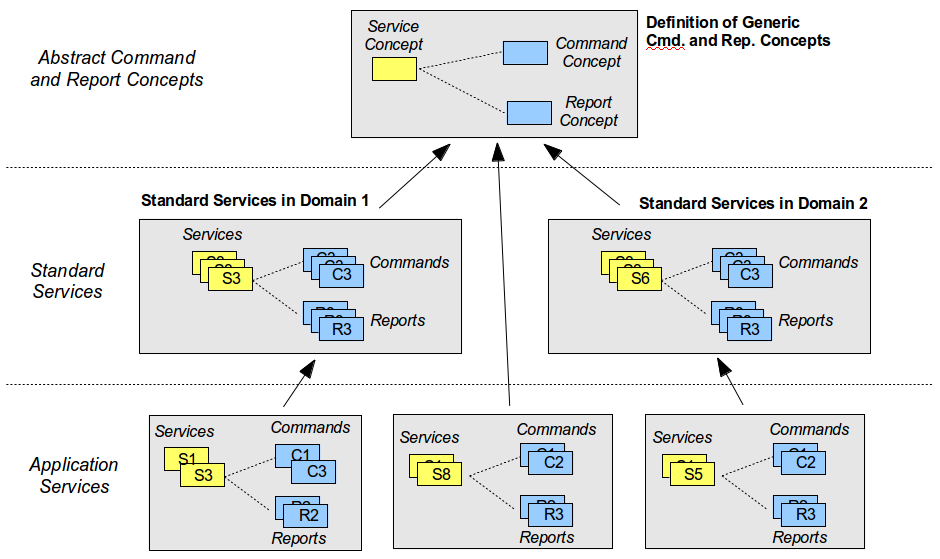
\includegraphics[scale=0.38,keepaspectratio=true]{HierarchicalDefServ.png}
 \caption{Hierarchical Definition of Services}
 \label{fig:HierarchicalDefServ}
\end{figure}

%-----------------------------------------------------------------------------------
\subsection{Objectives of C2 Implementation}\label{sec:ObjectivesC2Impl} 

The CORDET Framework is specified in reference [CR-SP] as an implementation-independent framework.
The C2 Implementation is a C-language implementation of the framework in the sense that it provides C implementations of the CORDET Components.

The CORDET Framework supports the development of service-oriented applications \textit{at specification level} by providing concepts which facilitate the specification of such applications.
The C2 Implementation supports the development of the same applications \textit{at implementation level} by providing pre-defined components which facilitate the specification of the same applications.

%------------------------------------------------------------------------------------
\subsection{Relationship To Packet Utilization Standard (PUS)}\label{sec:RelationshipToPUS}
The Packet Utilization Standard or PUS is an application-level interface standard for space-based applications. 
It is specified in reference [PS-SP]. 
In spite of its origin in the space industry, the PUS is suitable for a wide range of embedded control applications. 
In view of its long heritage and its proven ability to cover the interface needs of mission-critical systems of distributed applications, the PUS  has been used as a basis for the CORDET Framework in the sense that the service concept on which the CORDET Framework is based (see section \ref{sec:ServConcept}) is the same as the service concept specified by the PUS. 

In order to understand the degree of overlap between the PUS and the CORDET Framework, it is helpful to identify and contrast their respective concerns (the remainder of this section can be omitted by readers without a background in the space industry).

The PUS has two concerns: (a) it standardizes the semantics of the commands and reports which may be sent to or received from an application, and (b) it standardizes the external representations of these commands and reports (i.e. it specifies the layout of the packets which carry the commands and reports). 
The CORDET Framework shares the first concern in the sense that it uses the same service concept as the PUS but it does not share the second concern because it does not specify the external representation of commands and reports. 
Instead, the CORDET Framework specifies their internal representation (i.e. it predefines components to encapsulate commands and reports within an application) and it treats their serialization to, and de-serialization from, physical packets as an adaptation point to be resolved at application level.  
 
Thus, the CORDET Framework can be used to instantiate applications which are PUS-compliant but it is not restricted to PUS-compliant applications because it could be used to instantiate an application which uses a different external representation for its commands and reports than is specified by the PUS.

Table \ref{tab:PusCrConcerns} summarizes the concerns of the CORDET Framework and of the PUS.

\begin{longtable}{|>{\raggedright\arraybackslash}p{3cm}|p{10cm}|}
\caption{Concerns of CORDET Framework and of PUS}\label{tab:PusCrConcerns} \\
\hline
\rowcolor{light-gray}
\textbf{Concern} & \textbf{Coverage in CORDET Framework and PUS}\\
\hline\hline
\endfirsthead
\rowcolor{light-gray}
\textbf{Concern} & \textbf{Coverage in CORDET Framework and PUS}\\
\hline\hline
\endhead
Service Concept & CORDET Framework uses the same service concept as the PUS.\\
\hline
External Representation of Commands and Reports & The PUS specifies the external representation of its commands and reports (i.e. it specifies the layout of the packets carrying the commands and reports). The CORDET Framework does not specify the external representation of its commands and reports.\\
\hline
Internal Representation and Handling of Commands and Reports & The PUS does not specify how its commands and reports should be represented and handled inside an application. The CORDET Framework specifies the components representing the commands and reports in an application and the components required to handle them within that application.\\
\hline
\end{longtable}

In addition to the service concept, the PUS also defines the concept of \textit{application process} which is matched in the CORDET Framework by the concept of \textit{application}. The two concepts, though overlapping, have slightly different meanings. In the PUS, an application process is a source of reports and a sink for commands (see section 4.2.1 of reference [PS-SP]). In the CORDET Framework, an application is a node within a CORDET service-based distributed system. A CORDET application may therefore be both a source and a destination for both commands and reports. 

Generally speaking, a CORDET application may contain several PUS application processes. In order to allow multiple PUS application processes to be mapped to a single CORDET application, the CORDET Framework has introduced the concept of \textit{group}. Commands and reports in an application must belong to a group. A PUS application process may thus be represented within a CORDET application by a group. This is done by defining a group for each application process and by allocating all the commands and reports belonging to an application process to the same group. CORDET systems which do not aim at PUS compliance will normally not need the group concept and may just define one single group to which all commands and reports in the system belong by default.

%-------------------------------------------------------------------------------------------
\subsection{Middleware Layer}\label{sec:MwLayer} 
The CORDET Framework is an application-level framework and its domain is the management of services. Service messages encapsulating commands and reports are exchanged between applications. The mechanism through which these messages are sent from one application to another is outside the scope of the framework. The framework assumes that a \textit{middleware layer} is present which can be used to send and receive messages to and from other applications. 

Commands and reports travel on the middleware as \textit{packets}. A packet is an ordered sequence of bytes that contains all the information required to reconstruct a report or command. The layout of command and report packets is not specified by the CORDET Framework. An example of command and packet layout is specified in reference [PS-SP].

The process whereby a command or report is transformed into its packet is called \textit{serialization}. The inverse process whereby a command or report is interpreted and the equivalent report or command is reconstructed is called \textit{deserialization}.

The assumptions made by the framework about the middleware are specified in section \ref{sec:MwAssumptions}. The general concept is shown in figure \ref{fig:Middleware}. The CORDET Framework only covers the yellow boxes shown in the figure which represent the service-aware parts of a system.

\begin{figure}[ht]
 \centering
 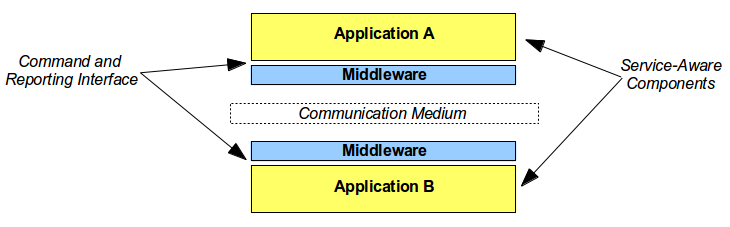
\includegraphics[scale=0.4,keepaspectratio=true]{Middleware.png}
 \caption{Applications and Middleware}
 \label{fig:Middleware}
\end{figure}


%=============================================================================================
\section{State Machine and Procedure Model}\label{sec:SmAndPrModel}
The C2 Implementation implements the specification of the CORDET Framework given in reference [CR-SP]. The behaviour of the CORDET Framework is specified through \textit{state machines} and \textit{procedures}. The semantics of the state machines and procedures in reference [CR-SP] is that of the \textit{FW Profile} of reference [FW-SP]. The FW Profile is a restriction of UML. It retains a simple but unambiguous subset of the UML features. Its state machines match the functional part of UML's state machines and its procedures match the functional part of UML's activity diagrams. 

The C2 Implementation uses the C1 Implementation of reference [FW-SP]. This is a library of C-language functions which implement the state machine and procedure concepts of the FW Profile. The C2 Implementation wraps all calls to functions of the C1 Implementation. Hence, in most cases, users will not need to interact with C1 Implementation functions.

Syntactically, a state machine in the C2 Implementation is represented by a variable of type \texttt{FwSmDesc\_t}. This type is a pointer to a structure (the \textit{state machine descriptor}) which holds all the information required to describe the state machine (its states and pseudo-states, its actions, its guards, and its transitions) and its current state. 

Similarly, a procedure in the C2 Implementation is represented by a variable of type \texttt{FwPrDesc\_t}. This type is a pointer to a structure (the \textit{procedure descriptor}) which holds all the information required to describe the procedure (its nodes, its actions, and its guards) and its current state. 

Users do not need to understand the internal structure of either the state machine or procedure descriptor.

%-------------------------------------------------------------------------------------------
\subsection{State Machine Extension}\label{sec:SmExtension} 
The C1 Implementation supports an extension mechanism for state machines which is similar to the inheritance-based extension mechanism of object-oriented languages. The C2 Implementation relies on this extension mechanism.

This section presents a brief overview of the state machine extension mechanism. More details can be found in reference [FW-SP]. 

A state machine (the \emph{base state machine}) can be \emph{extended} to create a new state machine (the \emph{derived state machine}). Initially, after being created, a derived state machine is a clone of its base (it has the same states with the same actions linked by the same transitions with the same actions and guards as the base state machines). The derived state machine can then be configured by performing one or more of the following operations: 

\begin{itemize}
\item Overriding one or more of its actions 
\item Overriding one or more of its guards 
\item Embedding new state machines in its states
\end{itemize}

The extension mechanism is useful where there is a need to define a large number of state machines which share the same topology (same set of states, of choice pseudo-states, and of transitions) but differ either in their actions, or in their guards, or in the internal behaviour of their states.

As an example consider the CORDET Components. All these components share the same initialization and reset logic which is described in section \ref{sec:BaseCmp} but they differ from each other in the specific actions and checks which they perform when they are initialized or reset. The C2 Implementation accordingly defines a base state machine to capture the generic behaviour of all components (see figure \ref{fig:BaseSM}) and then extends this base state machine to create the state machines representing specific component types. 

Using an object-oriented terminology, one could say that the C2 Implementation offers a base class implementing the generic initialization and reset behaviour of all components and it offers derived classes to represent the initialization and reset behaviour of specific component types.

Note, finally, that the C1 Implementation also supports an extension mechanism for procedures as well as for state machines. This procedure extension mechanism is not used in the C2 Implementation and is therefore not discussed further in this document. 

%=============================================================================================
\section{Component Model}\label{sec:CmpModel}\label{sec:BaseCmp}
The C2 Implementation is organized as a set of \textit{adaptable components}. The components provided by the C2 Implementation are called \textit{Framework Components}. A Framework Component consists of:

\begin{itemize}
\item A state machine derived\footnote{The term "derived" is used here in the sense of section \ref{sec:SmExtension}} from the \textit{Base State Machine} of figure \ref{fig:BaseSM};
\item The procedures which are started or executed by this state machine;
\item Any other procedure which supports the operation of this state machine.
\end{itemize}

The Base State Machine defines the process through which a component is initialized and configured. Thus, the definition of a Framework Component implies that all Framework Component share the same initialization and reset logic. 

\begin{figure}[h]
 \centering
 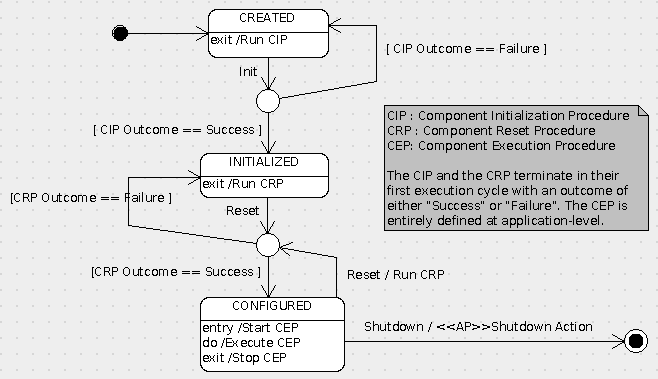
\includegraphics[scale=0.45,keepaspectratio=true]{BaseSM.png}
 \caption{Base State Machine}
 \label{fig:BaseSM}
\end{figure}

The logic of the Base State Machine is as follows. Initially, after being instantiated, framework components are in state CREATED. The hosting application is then expected to provide to each component the information it needs to perform its initialization. The type of this information is component-specific. After the necessary information has been provided, the application sends an \texttt{Init} command to the component. The component responds by running its \textit{Initialization Procedure}. This procedure is responsible for initializing the component and is defined in figure \ref{fig:InitializationAndReset}. 

The \textit{Initialization Procedure} is based on an \textit{Initialization Check} and an \textit{Initialization Action}. Both the check and the action are adaptation points which must be defined for each individual component. The Initialization Check normally checks that all parameters required for the component initialization have legal values.  The Initialization Action is only performed if the Initialization Check was successful.  This action normally creates all data structures required by the component and it performs other initialization actions as required. The Initialization Action can either fail or succeed.

The Initialization Procedure terminates in one single cycle with an outcome of either “Success” of “Failure”. Only the “Success” outcome is nominal and leads to the component making a transition to state INITIALIZED.

After successful initialization, the application provides to the component the information required to configure it and then sends a \texttt{Reset} command to it. The component responds by running its \textit{Reset Procedure}.  This procedure is responsible for configuring the component and is defined in figure  \ref{fig:InitializationAndReset}.
 
The \textit{Reset Procedure} is based on a \textit{Configuration Check} and a \textit{Configuration Action}. Both the check and the action are adaptation points which must be defined for each individual componet. The Configuration Check normally checks that all parameters required for the component configuration have legal values.  The Configuration Action is only performed if the Configuration Check was successful. This action normally initializes the value of all data structures required by the component and it performs other configuration actions as required. The Configuration Action can either fail or succeed.

The Reset Procedure terminates in one single cycle with an outcome of either “Success” of “Failure”. Only the “Success” outcome is nominal and leads to the component making a transition to state CONFIGURED.

\begin{figure}[ht]
 \centering
 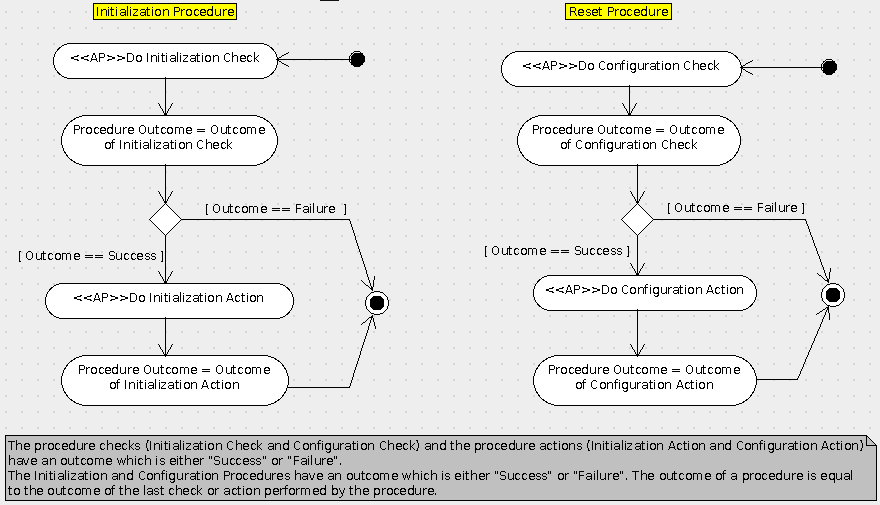
\includegraphics[scale=0.4,keepaspectratio=true]{InitializationAndReset.png}
 \caption{Initialization and Reset Procedures}
 \label{fig:InitializationAndReset}
\end{figure}

State CONFIGURED is the normal operational state of a component. In this state, the component executes its \textit{Execution Procedure}. This procedure must be entirely defined at application level. 

A component can be reset at any time by sending it command \texttt{Reset}. Nominally, this results in the component executing again its configuration actions and re-entering its CONFIGURED state. However, if any of the component parameters are found to have non-nominal values or if any of the configuration actions fail, then the component makes a transition to state INITIALIZED. This is a non-nominal situation.

Thus, the distinction between initialization actions and configuration actions is that the former are actions that, nominally, are performed only once during the life of an application whereas the latter are actions which may be performed more than once.

Note that there is no distinction between the actions that are performed when a component is configured for the first time during application start-up and the actions that are performed when a component is reset at run-time. This is intentional because resetting a component should bring it to the same state in which it was when the application had completed its start-up.

All framework components implement the behaviour defined by the Base State Machine. In general, the “meaningful” behaviour of a framework component is defined within the CONFIGURED state. This “meaningful” behaviour is defined either by implementing an \textit{Execution Procedure} or by embedding a state machine within the CONFIGURED state.

Components are shut down by sending them command \texttt{Shutdown}. This command results in the shutdown action being executed on the component. This action undoes the effects of the component initialization. Note that components can only be shutdown from state CONFIGURED. This is because the \texttt{Shutdown} operation models an orderly shutdown which should only be performed after an application has successfully completed its start-up. 

The C2 Implementation provides default implementations for the actions and checks of the Initialization and Reset Procedures and for the Execution Procedure:

\begin{itemize}
\item The default Initialization Check always returns "success".
\item The default Initialization Action sets the action outcome to "success" and then returns.
\item The default Configuration Check always returns "success".
\item The default Configuration Action sets the action outcome to "success" and then returns.
\item The default Execution Procedure executes the same empty action node at every cycle.
\end{itemize}

These defaults may be overridden when the Base Component is extended to create other Framework Components. Application developers will normally never use a Base Component directly (they only use components derived from the Base Component). 

%-------------------------------------------------------------------------------------------
\subsection{Component Hierarchy}\label{sec:CmpHierarchy} 
Figure \ref{fig:CmpHierarchy} show the components offered by the C2 Implementation in their hierarchical relationship. The Base Component at the top of the hierarchy encapsulates the Base State Machine. This component is not used directly. It only serves as a base from which the other components are derived.

Table \ref{tab:CmpList} lists the components offered by the C2 Implementation. Each component is described in a dedicated section of this document. Each component is implemented in a dedicated C-module. The rightmost column in the table gives the name of the C module.

\begin{figure}[H]
 \centering
 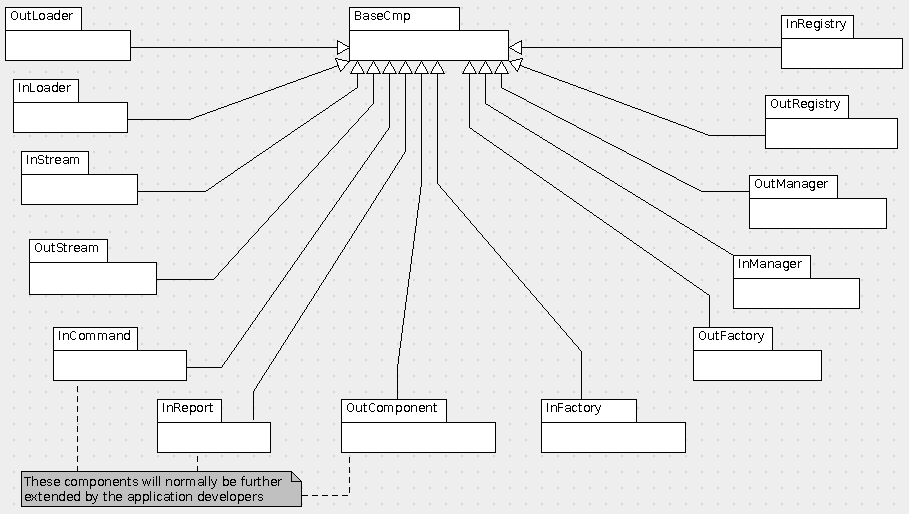
\includegraphics[scale=0.45,keepaspectratio=true]{CmpHierarchy.png}
 \caption{Component Hierarchy}
 \label{fig:CmpHierarchy}
\end{figure}

\begin{longtable}{|p{2.4cm}|p{7.5cm}|p{2.7cm}|}
\caption{List of Framework Components} \label{tab:CmpList}\\
\hline
\rowcolor{light-gray}
\textbf{Name} & \textbf{Function Within Framework} & \textbf{C-Module} \\
\hline\hline
\endfirsthead
\rowcolor{light-gray}
\textbf{Name} & \textbf{Function Within Framework} & \textbf{C-Module} \\
\hline\hline
\endhead
Base & Base component from which all framework components are derived. See section \ref{sec:CmpInst}. & \texttt{CrFwBaseCmp} \\
\hline
InStream & Reception of incoming commands and reports from communication middleware. See section \ref{sec:InStream}. & \texttt{CrFwInStream} \\
\hline
OutStream & Serializazion of outgoing commands and reports to the communication middleware. See section \ref{sec:OutStream}. & \texttt{CrFwOutStream} \\
\hline
InReport & Encapsulation of an incoming report. See section \ref{sec:InReport}. & \texttt{CrFwInRep} \\
\hline
InCommand & Encapsulation of an incoming command. See section \ref{sec:InCommand}. & \texttt{CrFwInCmd} \\
\hline
OutComponent & Encapsulation of an outgoing command or report. See section \ref{sec:OutComponent}. & \texttt{CrFwOutCmp} \\
\hline
InFactory & Dynamic creation of InCommands and InReports. See section \ref{sec:CmpImpl}. & \texttt{CrFwInFactory} \\
\hline
OutFactory & Dynamic creation of OutComponents. See section \ref{sec:CmpImpl}. & \texttt{CrFwOutFactory} \\
\hline
InLoader & Loading and re-routing of incoming commands and reports. See section \ref{sec:InLoader}. & \texttt{CrFwInLoader} \\
\hline
OutLoader & Loading of out-going command and reports into an OutStream. See section \ref{sec:OutLoader}. & \texttt{CrFwOutLoader} \\
\hline
InManager & Execution and processing of incoming commands and reports. See section \ref{sec:InManager}. & \texttt{CrFwInManager} \\
\hline
OutManager & Processing of outgoing commands and reports. See section \ref{sec:OutManager}. & \texttt{CrFwOutManager} \\
\hline
InRegistry & Tracking of the state of incoming commands and reports. See section \ref{sec:InRegistry}. & \texttt{CrFwInRegistry} \\
\hline
OutRegistry & Tracking of the state of outgoing commands and reports. See section \ref{sec:OutRegistry}. & \texttt{CrFwOutRegistry} \\
\hline
\end{longtable}


%-------------------------------------------------------------------------------------------
\subsection{Component Implementation}\label{sec:CmpImpl} 

Each component is implemented in either one single C module or in a small number of C modules. The modules implementing a component are gathered in a dedicated sub-directory which carries the name of the component. Thus, for instance, the modules implementing the Base Component are stored in a sub-directory called: \texttt{src/CrFramework/BaseCmp}.

From a syntactical point of view, a Framework Component is represented by the descriptor of its state machine (a variable of type \texttt{FwSmDesc\_t}, see section \ref{sec:SmAndPrModel}). Thus, syntactically, all framework components are of the same type (i.e. they are all represented by variables of type \texttt{FwSmDesc\_t}). 

Framework Components are instantiated by \textit{factory functions} which are provided by the framework. A factory function is a function with a name either like: \texttt{CrFwXxxMakeYyy} or like: \texttt{CrFwXxxMake}. The meaning of the strings 'Xxx' and 'Yyy' is discussed in section  \ref{sec:CmpInst}.

Components which are instantiated from the same factory function are said to be of the same \textit{component type}. Thus, each factory function defines a component type. Each component instance carries a \textit{type identifier} which uniquely identifies its type. The type identifier can be accessed with function \texttt{CrFwCmpGetTypeId}.

When a component instance is created, it is assigned an \textit{instance identifier} which uniquely identifies a component instance within the set of components of a certain type. The first instance to be created by a factory function is assigned the instance identifier of 0. The second instance is assigned the instance identifier 1. And so on. The instance identifier can be accessed with function \texttt{CrFwCmpGetInstanceId}.

There is a limited number of standard operations which can be performed on a framework component (executing it, querying it for its state, etc). An operation is performed by calling a function on the component. Table \ref{tab:CmpOperations} lists the most common such functions. 

Some of the functions listed in the table are only intended to operate upon a component instance of a certain type. For instance, function \texttt{CrFwInStreamGetPckt} should only be called with an argument representing an InStream component. This constraint cannot be enforced statically because, as indicated above, all components have the same syntactical type (they are all instances of type \texttt{FwSmDesc\_t}). It is therefore the responsibility of the application to enforce this constraint. The error arising when a function is called with a component of the incorrect type is not handled by the C2 Implementation. 

Although type checking is not possible statically owing to the limitations of the implementation language, it could be performed at run-time using the type information which every component carries with itself. Thus, functions could be modified or extended through a wrapper to check that the argument which they receive is of the expected type and to raise an error if this is not the case. 

\begin{longtable}{|p{5.5cm}|p{7.7cm}|}
\caption{List of Framework Component Operations} \label{tab:CmpOperations}\\
\hline
\rowcolor{light-gray}
\textbf{Operation} & \textbf{Description} \\
\hline\hline
\endfirsthead
\rowcolor{light-gray}
\textbf{Function} & \textbf{Description of Operation} \\
\hline\hline
\endhead
\texttt{CrFwCmpExecute($\langle$Inst$\rangle$)} & Execute the state machine of the component instance \texttt{Inst}. \\
\hline
\texttt{CrFwCmpInit($\langle$Inst$\rangle$)} & Initialize the Base State Machine of the component instance \texttt{Inst}. \\
\hline
\texttt{CrFwCmpReset($\langle$Inst$\rangle$)} & Reset the Base State Machine of the component instance \texttt{Inst}. \\
\hline
\texttt{CrFwCmpShutdown($\langle$Inst$\rangle$)} & Shutdown the Base State Machine of the component instance \texttt{Inst}. \\
\hline
\texttt{CrFwCmpIsInCreated($\langle$Inst$\rangle$)} & Return true if the Base State Machine of the component instance \texttt{Inst} is in state CREATED. \\
\hline
\texttt{CrFwCmpIsInInitialized($\langle$Inst$\rangle$)} & Return true if the Base State Machine of the component instance \texttt{Inst} is in state INITIALIZED. \\
\hline
\texttt{CrFwCmpIsInConfigured($\langle$Inst$\rangle$)} & Return true if the Base State Machine of the component instance \texttt{Inst} is in state CONFIGURED. \\
\hline
\texttt{CrFw$\langle$Type$\rangle\langle$Cmd$\rangle$($\langle$Inst$\rangle$)} & Send command \texttt{Cmd} to the state machine embedded in state CONFIGURED of the component instance \texttt{Inst} of type \texttt{Type}. \\
\hline
\texttt{CrFw$\langle$Type$\rangle$IsIn$\langle$State$\rangle$($\langle$Inst$\rangle$)} & Return true if the state machine embedded in state CONFIGURED of the component instance \texttt{Inst} of type \texttt{Type} is in state \texttt{State}. \\
\hline
\texttt{CrFwCmpGetInstanceId($\langle$Inst$\rangle$)} & Return the instance identifier of the component instance \texttt{Inst}. \\
\hline
\texttt{CrFwCmpGetTypeId($\langle$Inst$\rangle$)} & Return the type identifier of the component instance \texttt{Inst}. \\
\hline
\end{longtable}

%-----------------------------------------------------------------------------------------
\subsection{Component Data}\label{sec:CmpData}
 
A component instance is a variable of type \texttt{FwSmDesc\_t}. This type is defined by the C1 Implementation (see reference [FW-SP]). It represents a pointer to the \textit{state machine descriptor}.

The state machine descriptor consists of two parts (see figure \ref{fig:CmpData}). The first part (in yellow in the figure) is defined by the C1 Implementation and is the same for all state machines. This part holds the information about the state machine topology (its states, pseudo-states and transitions), its actions and guards, and its current state. The last field of this first part of the state machine descriptor is a pointer to the \textit{component data} (shown in light blue in the figure). 

The component data is the second part of the state machine descriptor. It consists of a data structure of type \texttt{CrFwCmpData\_t}. This data structure is in turn divided into two parts. The upper segment holds the data which are common to all framework components, namely:

\begin{itemize}
\item The component instance identifier
\item The component type identifier
\item The outcome of the last action executed by the component
\item The pointers to the Initialization, Reset and Execution Procedures of the component (see figure \ref{fig:BaseSM} -- it is recalled that these procedures are common to all framework components)
\end{itemize}

The lower segment of the component is a pointer to the \textit{component-specific data} (shown in green in the figure) namely data which are only used by components of a certain type. Syntactically, this type-specific data is implemented as a pointer to \texttt{void} which must be cast to a pointer to a structure. The type of the structure depends on the component type. These structure types are defined in \texttt{CrFwConstants.h}.

\begin{figure}[h]
 \centering
 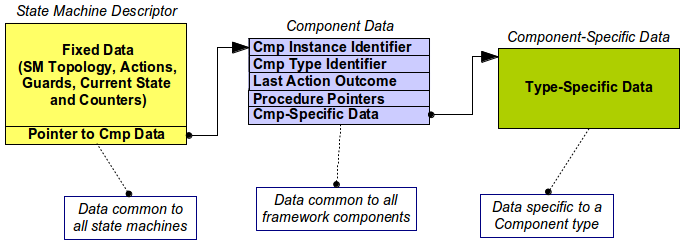
\includegraphics[scale=0.48,keepaspectratio=true]{CmpData.png}
 \caption{Component Data}
 \label{fig:CmpData}
\end{figure}

%-----------------------------------------------------------------------------------------
\section{Adaptation Model}\label{sec:AdaptationModel}
The C2 Implementation offers a set of generic components which application developers can use to build their applications. These components must be adapted to fit the needs of the end applications. The points where the component behaviour can be adapted are called \textit{Adaptation Points}.

The Adaptation Points are therefore the points where application developers may modify the pre-defined behaviour of the framework components. In some cases, the C2 Implementation pre-defines a default value for an Adaptation Point which application developers may either take unchanged or may modify. In other cases, no default behaviour is defined at framework level. 

Four types of Adaptation Points (AP) are supported by the C2 Implementation:

\begin{itemize}
\item Define Constant: a framework component uses a \texttt{\#DEFINE} constant whose value may be overridden by application developers.
\item Define Function: a framework component uses a function pointer and application developers must provide an implementation for the missing function (or, if available, may choose to use the default implementation provided at framework level)
\item Implement Interface: the framework defines an interface as a C header file and application developers must provide an implementation for it.
\item Define Type: a framework component uses a variables of a type defined as a \texttt{typedef} and application developers may override the default type definition.
\end{itemize}

The adaptable part of the framework is located in the \texttt{/cr/src/CrConfigTestSuite} directory of the C2 Implementation delivery (see section \ref{sec:InstAndContentOverview}. This directory holds: (a) a number of header files which define all the \texttt{\#DEFINE} constants and function pointers of the framework; and (b) a number of C body files which implement the interfaces which are left open at framework level. Thus, during the framework instantiation process, application developers adapt the framework components by updating the content of the files in the \texttt{/cr/src/CrConfigTestSuite} directory. The initial content of these files in the C2 Implementation delivery is that used for the Test Suite of the C2 Implementation (see \ref{sec:TestSuite}). 

Appendix \ref{sec:AdaptationPoints} lists the adaptation points of the framework component. Their detailed description is in the Doxygen documentation of the header and interface files which implement the adaptation points. 

Where applicable, the doxygen comments attached to the \texttt{\#DEFINE} constants and function pointers also identify their default values. For the implementation of the interface files, only test stubs are provided as default by the framework.

The default definitions of the \texttt{typedef} should be suitable for the vast majority of applications. Hence, in most cases, application developers may ignore them.

Manipulations of function pointers is fraught with dangers in C. It is therefore important to stress that, in the C2 Implementation, function pointers are exclusively used \textit{within} the framework components (where their use has been extensively checked and validated). Application developers will normally not have to use the framework function pointers and are therefore protected from the attendant risks.

Adaptation is done at compile-time only. During the framework instantiation process, the application developer closes the framework's adaptation points (or, where appopriate, takes over the default values defined at framework level). The choices made at this time cannot be modified at run-time: the C2 Implementation provides no mechanism to re-configure the framework dynamically. This limitation is dictated both by reasons of CPU and memory efficiency and by the desire to enhance static predictability of behaviour.

%=======================================================================================
\section{Application Start-Up and Shut-Down}\label{sec:AppStartUpAndShutdown}

The application start-up process is divided into two stages: \textit{initialization} and \textit{configuration}. The initialization stage covers actions which are performed only at start-up time and which cannot be repeated until the application (or a part of it) is shutdown. The configuration stage covers actions which are performed at start-up time but which may also be performed at a later stage if there is a need to reset either the entire application or a part of it. 

In the CORDET Framework document, the term \textit{shutdown} is used to designate the orderly shutdown of an application or of a component. Obviously, applications and components may also undergo an emergency shutdown. This is entirely uncontrolled and is not covered in any way by the CORDET Framework.

The start-up and shutdown processes are specified at two levels: at the level of \textit{individual components} and at the level of the \textit{entire application} which are described in, respectively, sections \ref{sec:CmpModel} and \ref{sec:AppStartUp}.

Before they are initialized and configured, components must be \textit{instantiated}. Most components required by an application are instantiated as part of that application start-up (\textit{early component instantiation}). In some cases, components may need to be instantiated during the application's normal operation (\textit{late component instantiation}). The two forms of components instantation are discussed in section \ref{sec:CmpInst}.

%-----------------------------------------------------------------------------------------
\subsection{Component Instantiation}\label{sec:CmpInst}
Components may be instantiated either \textit{early} or \textit{late}. Early instantiation takes place as part of the application start-up. This is required by the logic of the \textit{Application State Machine} of section \ref{sec:AppStartUp}.

Late instantiation can take place at any time during the application's normal operation (i.e. while the \textit{Application State Machine} of section \ref{sec:AppStartUp} is in state NORMAL). Late instantiation is only foreseen for components which encapsulate commands or reports. These components must be created during the normal operation phase of an application because commands and reports are sent and received dynamically by an application. All other components are instantiated during the application start-up phase (early instantiation).

Component instantiation (both early and late) is done through \textit{factory functions} which are provided by the framework. For components subject to early instantiation, factory functions have names like \texttt{CrFwXxxMake} where 'Xxx' is the name of the component type. Thus, for instance, the factory function which generates InStream components is called \texttt{CrFwInStreamMake}.  

Only a fixed and statically pre-defined number of instances of components can be instantiated statically. If only one instance may be instantiated (singleton components), the factory function \texttt{CrFwXxxMake} takes no argument. The first time it is called, it creates the singleton instance. Subsequent calls return the same instance.

If N instances may be instantiated (with N greater than 1), the factory function \texttt{CrFwXxxMake} takes as argument an integer in the range 0 to N-1. The first time the function is called with an argument i, the function creates the (i+1)-th instance of the component. Subsequent calls with the same argument value return the same instance. An out-of-range value of the argument results in the function returning NULL. If this is an error situation, it must be handled by the caller (i.e. the factory function itself does not perform any error handling for an out-of-limit argument).

For non-singleton components, the maximum number of instances which can be created is an adaptation point.

The memory resources for the components subject to early instantiation are allocated through calls to \texttt{malloc}. This is acceptable because these calls are only performed in the application start-up phase and for a fixed and statically pre-defined number of times. Hence, it is possible to guarantee by static analysis that all \texttt{malloc} calls will succeed and predictability of behaviour is thus ensured (see also discussion in section \ref{sec:MemMng}).

The instantiation of a component subject to early instantiation is irreversible: the resources which are allocated to the component will only be released if the application is terminated. Note in particular that the Shutdown Procedure of the Application Start-Up State Machine (see section \ref{sec:AppStartUp}) does \underline{not} release the resources claimed during the early component instantiation process. 

For components subject to early instantiation, factory functions are provided by factory components and have names like \texttt{CrFwYyyMakeXxx} where 'Xxx' is the name of the component type and 'Yyy' is the name of the factory component. Thus, for instance, components encapsulating incoming commands are generated by the factory function \texttt{CrFwInCmdFactoryMakeInCmd} which belongs to the factory component InCmdFactory.  

The CORDET Framework defines two factory components: the OutFactory to instantiate components encapsulating out-going commands and reports and the InFactory to instantiate component encapsulating incoming commands and reports (see the overview in sections \ref{sec:ManagementOfOutGoingCmdAndRep} and \ref{sec:ManagementOfIncomingCmdAndRep}. The C2 Implementation implements these factories in modules \texttt{CrFwOutFactory} and \texttt{CrFwInFactory}. 

In addition to the \texttt{Make} function which creates a new component instance, factory components also offer \texttt{Release} functions with names like \texttt{CrFwYyyReleaseXxx}. The \texttt{Release} functions take a component instance as argument and reclaim the resources allocated to that component instance.

As part of their initialization, factory components pre-allocate a pool of memory. When they receive a \texttt{Make} request, they allocate memory for the component-to-be-instantiated from this pool. The memory is released when the user of the component instance calls \texttt{Release}. The memory allocation algorithm is deterministic. Each factory can only create a fixed number of component instances (the factory's \textit{capacity}). A \texttt{Make} request at a time when all factory instances are already in use will fail by returning \texttt{NULL}. The capacity of a factory is an adaptation point.

Note that, if a failure of the \texttt{Make} operation represents an error, this must be handled by the user of the factory. The factory itself does not perform any error handling.

%----------------------------------------------------------------------------------------
\subsection{Application Start-Up}\label{sec:AppStartUp}
The CORDET Framework defines the Application State Machine of figure \ref{fig:ApplicationSM} to model the start-up and shutdown logic of an application. 

When the application is created, the Application State Machine is in state START\_UP. 
In this state, the \textit{Application Start-Up Procedure} is executed. 
This procedure is entirely defined at application level but is subject to two constraints: (a) the procedure must include the instantiation, initialization and configuration of all components subject to early instantiation, and (b) the procedure may only terminate if successful configuration of all components subject to early instantiation is confirmed (i.e. if all these components are in state CONFIGURED). 

Normal operation takes place in state NORMAL. 
In particular, the services provided by an application to its users are only guaranteed to be available when the application is in state NORMAL and it is only from this state that the application makes use of the services provided by other applications. 
Thus, in state NORMAL, an application may assume that its service interfaces are all operational.

An application can be reset by sending command \texttt{Reset} to its \textit{Application State Machine}. This causes a transition to state RESET where the \textit{Application Reset Procedure} is executed. This procedure is entirely defined at application level but is subject to two constraints: (a) the procedure must include the sending of the \texttt{Reset} command to all currently instatiated components, and (b) the procedure may only terminate if all currently instantiated components are in state CONFIGURED.

It follows from the logic outlined above that, when the application is in state NORMAL, all its statically instantiated components are guaranteed to be correctly configured (i.e. they are guaranteed to be in state CONFIGURED).

The \textit{Application Start-Up Procedure} and the \textit{Application Reset Procedure} will normally share much behaviour but they may not coincide because there may be some actions which are only executed once when an application is started up (such as, for instance, the initialization of all application components).

Finally, the orderly shutdown of an application is performed by sending command \texttt{Shutdown} to the \textit{Application State Machine}. This triggers a transition to state SHUTDOWN where the \textit{Application Shutdown Procedure} is executed. This procedure is entirely defined at application level but is subject to one constraint: the procedure must include the sending of the \texttt{Shutdown} command to all currently instantiated components. 

\begin{figure}[ht]
 \centering
 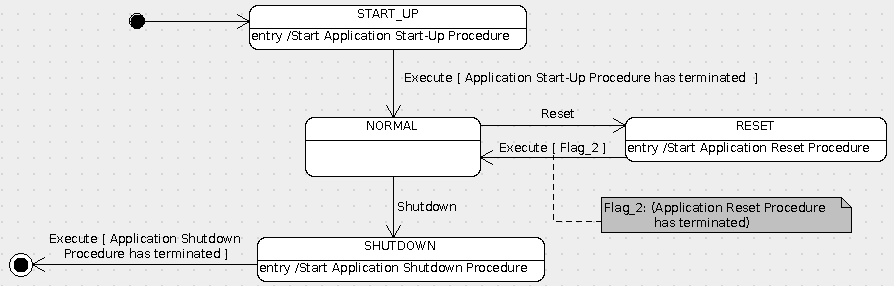
\includegraphics[scale=0.4,keepaspectratio=true]{ApplicationSM.png}
 \caption{Application State Machine}
 \label{fig:ApplicationSM}
\end{figure}

Applications may (and normally will) define embedded state machines in the states shown in figure \ref{fig:ApplicationSM}. In particular, applications normally have several operational states which would appear as sub-states of NORMAL.


The C2 Implementation implements the \textit{Application State Machine} in module \texttt{CrFwAppSm}. The three procedures controlled by the \textit{Application State Machine} are not provided by the C2 Implementation because they are application-specific. The C2 Implementation provides three header files \texttt{CrFwAppStartUpProc.h}, \texttt{CrFwAppResetProc.h}, and \texttt{CrFwAppShutdownProc.h} which defines the point of access to the three procedures. Application developers should provide implementations for these three header files as part of the framework instantiation process.

Also as part of the framework instantiation process, application developers may want to add behaviour to the four states of the \textit{Application State Machine} by embedding state machines within these states. Embedding of state machines is done using function \texttt{FwSmEmbed} defined by the C1 Implementation (see reference [FW-SP]).

%===========================================================================
\section{Command and Report Concepts}\label{sec:CmdAndRepModel}
This section describes the command and report concepts assumed by the CORDET Framework and implemented by the C2 Implementation. 

This section considers commands and reports at the abstract level only. The commanding and reporting concepts described here are therefore applicable to any command or report, irrespective of the specific service to which they belong or of the specific activities which the command triggers or of the specific information which the report carries. Concrete commands and reports are defined by applications according to their needs.These concrete commands and reports are defined as specializations of the generic command and report concepts described in the present section. 

%---------------------------------------------------------------------------------
\subsection{Command Concept }\label{sec:CmdConcept}
Each command belongs to a service. 
Within that service, the command is identified by the \textit{sub-type} (a positive integer). 
Thus, a command is fully identified by a pair [x,y] where 'x' is the identifier of the service to which the command belongs (the service type, see section \ref{sec:ServConcept}) and 'y' is the identifier of the command within the service (the command sub-type).

Commands are \textit{types} which are instantiated at run-time. 
A command is generated by a service user in order to trigger the execution of certain actions by the service providers. Thus, a command instance begins its life when the application on the service user side (the \textit{user application}) decides that it wishes to issue a request to the application on the service provider side (the \textit{provider application}). 

A command is sent by the user application to the provider application where it triggers the execution of certain actions. Before being sent to the provider application, the command is configured. Through the configuration process, the command acquires the information it will need to execute its actions. The command's actions in the provider application are executed in a sequence of steps which may extend over time. Both the sending of the command to its destination and the execution of its actions in the provider application are conditional upon certain checks being passed. The command encapsulates both the actions that must be executed and the conditional checks that determine whether the command is sent and whether its actions are executed.

The same command instance may be sent to its destination more than once. This models the situation where a user is issuing periodic requests to a service provider. In this case, the content of the command is updated every time the command is sent to its destination. It is a logical error to re-send a command instance to its destination before the actions triggered by the previous execution of the same command have completed.

A command is defined by its \textit{attributes}, its \textit{conditional checks}, and its \textit{actions}. 

Attributes designate characteristics that are entirely defined by their value. 
Actions and conditional checks designate executable functionalities that are associated to the command. 
Both actions and conditional checks are executed by the command as a result of changes in its internal state. 
The conditional checks are used to determine whether and when the command actions are executed.

The next three subsections further define the command attributes, the command conditional checks, and the command actions. The last sub-section describes the lifecycle of a command. 

%---------------------------------------------------------------------------------
\subsubsection{The Command Attributes}\label{sec:CmdAttributes}

An attribute is a characteristics that is entirely defined by its value. 
A command has the following attributes:

\begin{itemize}
\item \textbf{Service Type:} Each command contributes to implementing a service. This attribute identifies the service that the command implements. 

\item \textbf{Command Sub-Type}: Each service is implemented by several commands. 
This attribute identifies the type of the command within a certain service. 

\item \textbf{Command Identifier}: A command may exist in two distinct applications (the user application which sends the command and the provider application which receives it). This attribute uniquely identifies the command instance within both applications and throughout the life of both applications.

\item \textbf{Destination} Commands are generated by a user application for a provider application. This attribute identifies the provider application for which the command is intended.

\item \textbf{Source}
Commands are generated by a user application for a provider application. This attribute identifies the user application which issues the command.

\item \textbf{Time Stamp}:
The time when the user application makes the request to send the command to its destination. 

\item \textbf{Group}
Commands sent by a user application to the same destination are allocated to a group. This attribute identifies the group to which the command belongs. The concept of group is primarily relevant to applications which aim at PUS-compliance (see section \ref{sec:RelationshipToPUS}). 

\item \textbf{Sequence Counter}
Every time a user application issues a command belonging to a certain destination group, it increments a counter. The sequence counter attribute holds the value of this counter. The sequence counter can be used by the recipient application to check whether any commands addressed to it have been lost. 

\item \textbf{Acknowledge Level}
Command execution goes through four stages: acceptance, start, progress, and termination (see section 5.1.4). This attribute determines whether successful completion of each of these stages should be reported to the sender of the command. Note that failure to complete a stage is reported unconditionally.

\item \textbf{Progress Step Identifier}
On the service provider side, a command is executed in a sequence of progress steps. Each progress step is identified by a positive integer (but note that step identifiers are not necessarily in sequence). This attribute holds the identifier of the current step. A command must have at least one step. This attribute is only meaningful on the service provider side.

\item \textbf{Command Parameters}
Some commands may require parameters to fully specify the actions and checks that they encapsulate. The “Command Parameters” attribute holds the value of these parameters. This attribute consists of an ordered sequence of items of primitive type. 

\item \textbf{Discriminant}
The number and type of command parameters in a command instance is not necessarily determined by the command type (i.e. different instances of the same command type may have different sets of command parameters). The discriminant is a command parameter which determines the number and type of the other command parameters. 

Thus, the layout of a command instance is fully determined by the triplet: [x,y,z] where 'x' is the identifier of the service to which the command belongs (the service type), 'y' is the identifier of the command within the service (the command sub-type), and 'z' is the discriminant. 

The discriminant is an optional attribute. Command types which have no parameters, or which have a fixed set of parameters, have no discriminant.

\item \textbf{CRC}
A command carries a checksum which is set by the command's sender and which the recipient of the command can use to verify the integrity of the command's transmission. 
\end{itemize}

%---------------------------------------------------------------------------------
\subsubsection{The Command Conditional Checks}\label{sec:CmdCondChecks}

A conditional check is an executable functionality which returns an enumerated value. The enumerated value reports the outcome of the check. Conditional checks are performed as part of the processing of a command. Their outcome determines whether and when the command actions are preformed. Conditional checks must have zero logical execution time. This restriction allows them to be mapped to guards in state machines. 

Some checks are performed on the user's side (i.e. prior to the command being issued by the user application); others are performed on the provider's side (i.e. after the command has been received by the provider application). 

The following conditional checks are defined for a command on the service user side:

\begin{itemize}
\item \textbf{Enable Check}
This check is performed when the user application makes a request to send a command to the service provider. The enable check determines whether the command instance is enabled or disabled. If the command instance is disabled, then the command is aborted. If instead the command instance is enabled, it remains in a pending state until the ready check authorizes it being sent to its destination.

\item \textbf{Ready Check}
This check is performed on a pending command instance that has passed its enable check. The ready check determines when the command instance is sent to its destination.  The command instance remains pending until the ready check is passed. When the ready check is passed, the command instance may be sent to its destination. 

\item \textbf{Repeat Check}
This check is performed on a command instance after it has been sent to its destination. The check returns either "repeat" or "no repeat". In the former case, the command instance is updated and sent again to its destination. In the latter case, it is terminated.
\end{itemize}

On the service provider side, the following conditional checks are defined for a command:

\begin{itemize}
\item \textbf{Acceptance Check}
The acceptance check is performed when the command instance is received by its destination. If the acceptance check is passed, then the command remains pending and can be further processed by its recipient. If the acceptance check is not passed, then the command instance is aborted.

\item \textbf{Ready Check}
This check is performed on a pending command instance that has passed its acceptance check. The ready check determines when the execution of the command starts.  As long as the ready check is not passed, the command remains pending. When the ready check is passed, the command instance attempts to start execution.
\end{itemize}

%---------------------------------------------------------------------------------
\subsubsection{The Command Actions}\label{sec:CmdActions}
Command actions are executable functionalities which encapsulate the actions to be performed by the command. Command actions are executed depending on the outcome of the command conditional checks. Command actions must have zero logical execution time. This restriction allows them to be mapped to actions in state machines. 

The following action is defined for a command on the service user side:

\begin{itemize}
\item \textbf{Update Action}
Through this action, the command acquires the information which it requires to execute its action on the service provider application. This action is executed before the command is sent to its destination. If the command is sent more than once (i.e. if its repeat check returns "repeat" one or more times), then the Update Action is performed repeatedly every time the command must be sent to its destination.
\end{itemize} 

The following actions are defined for a command on the service provider side:

\begin{itemize}
\item \textbf{Start Action}
The start action is executed after the start check has been passed. The start action encapsulates one-off initialization actions that must be performed at the beginning of a command's execution. 
The start action has an outcome which is either “success” or “failed”. If the outcome of the start action is “failed”, the command is aborted. 
\item \textbf{Progress Action}
Commands execute in one or more execution steps. The progress action encapsulates the actions performed in one execution step. The progress action is executed the first time after the start action has terminated and it is then executed again until either it fails or it completes.
 
The progress action has two outcomes: a completion outcome which can be either "completed" or "not completed" and a success outcome which can be either "success" or "failed". If the completion outcome is "completed", then all execution steps have been completed and the termination action is executed. If, instead, it is "not completed", then another execution step will be executed. The success outcome determines the kind of acknowledge reports which are generated for the progress action. 

Finally, the progress action updates the progress step identifier. A "progress step" is a set of logically related execution steps which are executed in sequence.
\item \textbf{Termination Action}
The termination action is executed after all the progress steps have been successfully executed. The termination action encapsulates one-off finalization actions that must be performed before the command is terminated.
The termination action has an outcome which is either “success” or “failed”. If the outcome of the termination action is “failed”, the command is aborted. 
\item \textbf{Abort Action}
If a command is aborted (i.e. if it fails its acceptance check, or its start action faisl, or its progress action fails, or its termination action fails) then it executes its abort action. The abort action thus encapsulates the finalization actions to be performed in case of a command failure. 
\end{itemize}

%---------------------------------------------------------------------------------
\subsubsection{Command Lifecycle}\label{sec:CmdLifecycle}
A command instance begins its life on the user side when the user application makes a request for the command instance to be sent to the provider application. Nominally, on the user side, the command can be in one single state PENDING. This corresponds to the state of a command that has passed its enable check and is waiting for its ready check to authorize the transfer of the command to the provider application. 

On the provider side, the command instance passes through four states: ACCEPTED, STARTED, PROGRESS, and TERMINATED. The command states are entered in sequence as the command is executed. The PROGRESS state can be entered more than once to represent the fact that some commands execute actions which extend over time and which are therefore broken into several steps.

To each command state one check and one action may be associated. The checks determine whether a state can be entered or exited. For instance, if the acceptance check fails, then the command cannot be executed. The actions encapsulate the activities to be performed when the command enters a certain state. For instance, the start action defines the actions to be executed when the command is started. Actions have an outcome which determines the next step in the execution of the command.

On the provider side, a change in the state of a command is marked by the generation of an Acknowledge Report. Acknowledge Reports are used to notify the sender of a command of a change in the state of the command. Four kinds of Acknowledge Reports are defined corresponding to the four states that a command may have in a provider application:

\begin{itemize}
\item \textit{Acceptance Acknowledge Report} to notify the command sender of the outcome of the acceptance check.
\item \textit{Start Acknowledge Report} to notify the command sender of the outcome of the start action.
\item \textit{Progress Acknowledge Report} to notify the command sender of the outcome of a progress step.
\item \textit{Termination Acknowledge Report} to notify the command sender of the outcome of the termination action.
\end{itemize}

The sending of an acknowledge report to a command sender is done unconditionally in the following cases: (a) the acceptance check has not been passed, (b) the start action has failed, (c) the progress action has failed, or (d) the termination action has failed. Note that all of these cases result in the command being aborted. Thus, the sending of an acknowledge report is done unconditionally whenever a check or action results in a command being aborted. For instance, if the start action of a command fails, a Start Acknowledge Report is sent to the command sender to notify it that the command has failed to start execution and has consequently been aborted.

In all other cases (namely when the acceptance check is passed, or the start action, or the progress action, or the termination action are successful), the sending of the acknowledge report to the command sender is conditional upon the value of the Acknowledge Level attribute of the command (see section \ref{sec:CmdAttributes}). Thus, for instance, the command sender can set the Acknowledge Level attribute of a certain command such that only successful acceptance and successful termination of the command are reported. 

The Progress Acknowledge Report is only sent at the end of a progress step. A progress step is deemed to have ended when the previous execution of the progress action has resulted in the progress step identifier being updated.

Figure \ref{fig:CmdLifecycle} shows the nominal lifecycle of a command in an informal notation. In summary, the CORDET Framework pre-defines the logic to handle the transitions between the command states. It does this by defining the logic to manage the execution of the command checks and of the command actions but it leaves the definition of the content of the actions and checks open. 

The lifecycle outlined above may be repeated more than once for the same command instance. Repetition is determed by the outcome of the Repeat Check. The Repeat Check is performed at the end of the lifecycle depicted in figure \ref{fig:CmdLifecycle}. If it returns "no repeat", then the command instance is destroyed. If instead, the check returns "repeat", then the content of the command is updated and thze command is re-sent to its destination where it repeats the lifecycle of figure \ref{fig:CmdLifecycle}.

\begin{figure}[ht]
 \centering
 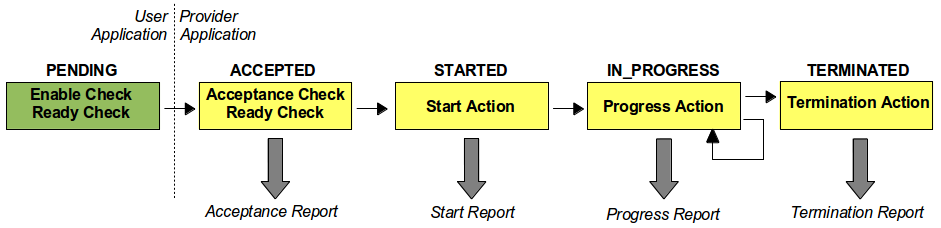
\includegraphics[scale=0.35,keepaspectratio=true]{CmdLifecycle.png}
 \caption{Command Lifecycle (Informal Notation)}
 \label{fig:CmdLifecycle}
\end{figure}




\subsubsection{Mapping to C-Level Constructs}\label{sec:CmdConceptMapping}
The C2 Implementation maps commands to software-level components as follows: out-going commands are mapped to OutComponent components which are implemented in the C module \texttt{CrFwOutCmp} (see section \ref{sec:OutComponent}); incoming commands are mapped to InCommand components which are implemented in the C module \texttt{CrFwInCmd} (see section \ref{sec:InCommand}). Table \ref{tab:CmdConceptMapping} shows how the attributes, conditional checks, and actions of commands are mapped to C-level constructs in the C2 Implementation. Note that, in most cases, the mapping depends on whether the command is out-going (i.e. the host application is a user application) or incoming (i.e. the host application is a provider application).

\begin{longtable}{|>{\raggedright}p{2.0cm}|p{11.3cm}|}
\caption{Mapping of Commands to C-Level Constructs} \label{tab:CmdConceptMapping}\\
\hline
\rowcolor{light-gray}
\textbf{Name} & \textbf{Mapping to C-Level Construct} \\
\hline\hline
\endfirsthead
\rowcolor{light-gray}
\textbf{Name} & \textbf{Mapping to C-Level Construct} \\
\hline\hline
\endhead
Service Type Attribute & \texttt{ServType} attribute in \texttt{CrFwOutCmp} and \texttt{CrFwInCmd} modules. Value set when component is created by its factory and accessible through getter function. \\
\hline
Command Sub-Type Attribute & \texttt{ServSubType} attribute in \texttt{CrFwOutCmp} and \texttt{CrFwInCmd} modules. Value set when component is created by its factory and accessible through getter function. \\
\hline
Command Identifier Attribute & \texttt{InstanceId} attribute inherited from base component \texttt{CrFwbaseCmp}. Value set when component is created by its factory and accessible through getter function. \\
\hline
Destination Attribute & \texttt{Dest} attribute in \texttt{CrFwOutCmp}, accessible through getter and setter functions. Attribute not explicitly present in \texttt{CrFwInCmd} since the destination of an InCommand is, by definition, the host application. \\
\hline
Source Attribute & \texttt{Src} attribute in \texttt{CrFwOutCmp} and \texttt{CrFwInCmd} modules. Value set when component is created by its factory and accessible through getter function. \\
\hline
Time Stamp Attribute & \texttt{TimeStamp} attribute in \texttt{CrFwOutCmp} module. Value accessible and controllable through getter and setter functions. Attribute is not present in \texttt{CrFwInCmd} module. \\
\hline
Group Attribute & \texttt{Group} attribute in \texttt{CrFwOutCmp} and \texttt{CrFwInCmd} modules. Value accessible and controllable through getter and setter functions in the \texttt{CrFwOutCmp} module and in read-only mode through a getter function in the \texttt{CrFwInCmd} module.  \\
\hline
Sequence Counter Attribute & \texttt{SeqCnt} attribute in \texttt{CrFwInCmd} module. Value set when the component is created by its factory and accessible through getter function. Attribute is not present in \texttt{CrFwOutCmp} module since the sequence counter of out-going commands is set at the time the command is sent out. \\
\hline
Acknowledge Level Attribute & \texttt{AckLevel} attribute in \texttt{CrFwOutCmp} and \texttt{CrFwInCmd} modules. Value controllable and accessible through setter and getter functions in \texttt{CrFwOutCmp} module but only accessible in read mode in \texttt{CrFwInCmd} module. \\
\hline
Discriminant Attribute & \texttt{Discriminant} attribute in \texttt{CrFwOutCmp} and \texttt{CrFwInCmd} modules. Value set when component is created by its factory and accessible through getter function. Update possible through a setter function in \texttt{CrFwOutCmp} module.  \\
\hline
Command Parameter Attributes & These attributes are application-specific.  \\
\hline
Enable Check & Function implementing the Enable Check Operation for an out-going command specified through a function pointer in the CR\_FW\_OUTCMP\_INIT\_KIND\_DESC initializer.  \\
\hline
Ready Check & Function implementing the Ready Check Operation for an out-going command specified through a function pointer in the CR\_FW\_OUTCMP\_INIT\_KIND\_DESC initializer. Function implementing the Ready Check Operation for an incoming command specified through a function pointer in the CR\_FW\_INCMD\_INIT\_KIND\_DESC initializer. \\
\hline
Repeat Check & Function implementing the Repeat Check Operation for an out-going command specified through a function pointer in the CR\_FW\_OUTCMP\_INIT\_KIND\_DESC initializer.  \\
\hline
Acceptance Check & The part of the acceptance check which verifies validity of the command type and availability of resources is implemented in the Load Command/Report Procedure of the InLoader (see section \ref{sec:InLoader}). The command-specific part of the acceptance check is implemented in the Validity Check Operation specified through a function pointer in the CR\_FW\_INCMD\_INIT\_KIND\_DESC initializer.  \\
\hline
Update Action & Function implementing the Update Action Operation for an out-going command specified through a function pointer in the CR\_FW\_OUTCMP\_INIT\_KIND\_DESC initializer.  \\
\hline
Start Action & Function implementing the Start Action Operation for an incoming command specified through a function pointer in the CR\_FW\_INCMD\_INIT\_KIND\_DESC initializer. \\
\hline
Progress Action & Function implementing the Progress Action Operation for an incoming command specified through a function pointer in the CR\_FW\_INCMD\_INIT\_KIND\_DESC initializer. \\
\hline
Termination Action & Function implementing the Termination Action Operation for an incoming command specified through a function pointer in the CR\_FW\_INCMD\_INIT\_KIND\_DESC initializer. \\
\hline
Abort Action & Function implementing the Abort Action Operation for an incoming command specified through a function pointer in the CR\_FW\_INCMD\_INIT\_KIND\_DESC initializer. \\
\hline
\end{longtable}


%---------------------------------------------------------------------------------
\subsection{Report Concept }\label{sec:RepConcept}
Each report belongs to a service. Within that service, the report is identified by the \textit{sub-type} (a positive integer). Thus, a report is fully identified by a pair [x,y] where 'x' is the identifier of the service to which the report belongs (the service type, see section \ref{sec:ServConcept}) and 'y' is the identifier of the report within the service (the command sub-type).

Commands and reports within the same service have different sub-types. Thus, it is not possible for a command and a report to be identified by the same [type, sub-type] pair.  

Reports are \textit{types} which are instantiated at run-time. A report is generated by a service provider which sends it to a service user in order to provide it with information about its internal state. Thus, a report instance begins its life when the application on the service provider side (the \textit{provider application}) decides that it wishes to send some information to the application on the service user side (the \textit{user application}). 

On the service provider side, a report is configured with the information that it must carry and then it is sent to its destination (a user application). The sending of the report to the user application may be conditional on certain checks being passed. On the user side, the report performs an update action. The report encapsulates the data to be sent, the conditional checks which determine whether the report is sent, and the update action.  

The same report instance may be sent to its destination more than once. This models the situation where a service provider is issuing periodic reports to a service user. In this case, the content of the report is updated every time it is sent to its destination. 

Thus, a report is defined by its \textit{attributes}, its \textit{conditional checks} and an \textit{update action}. 

Attributes designate characteristics that are entirely defined by their value. The update actions and conditional checks designate executable functionalities that are associated to the report. The conditional checks determine whether a report is sent to its destination and the update action determines what the report does with the data it carries in its destination.

The next three subsections further define the report attributes, the report conditional checks and the report update action. The last sub-section describes the lifecycle of a report. 

%---------------------------------------------------------------------------------
\subsubsection{The Report Attributes}\label{sec:RepAttributes}

An attribute is a characteristics that is entirely defined by its value. A report has the following attributes:

\begin{itemize}
\item \textbf{Service Type}
Each report contributes to implementing a service. This attribute identifies the service that the report implements. 
\item \textbf{Report Sub-Type}
Each service is implemented by several reports. This attribute identifies the type of the report within a certain service. 
\item \textbf{Report Identifier}
A report may exist in two distinct applications (the provider application which sends the report and the user application which receives it). This attribute uniquely identifies the report instance within both applications and throughout the life of both applications.
\item \textbf{Destination}
Reports are generated by a provider application for a user application. This attribute identifies the user application for which the report is intended.
\item \textbf{Source}
Reports are generated by a provider application for a user application. This attribute identifies the provider application which issues the report.
\item \textbf{Time Stamp}
The time when the provider application makes the request to send the report to its destination.
\item \textbf{Group}
Reports sent by a provider application to the same destination are allocated to a group. This attribute identifies the group to which the report belongs. The concept of group is primarily relevant to applications which aim at PUS-compliance (see section \ref{sec:RelationshipToPUS}).  
\item \textbf{Sequence Counter}
Every time a provider application generates a report belonging to a certain source group, it increments a counter. The sequence counter attribute holds the value of this counter. The sequence counter can be used by the recipient application to check whether any reports addressed to it have been lost. 
\item \textbf{Report Parameters}
Some reports may require parameters to fully specify the actions and checks that they encapsulate. The “Report Parameters” attribute holds the value of these parameters. This attribute consists of an ordered sequence of items of primitive type. 
\item \textbf{Discriminant}
The number and type of report parameters in a report instance is not necessarily determined by the report type (i.e. different instances of the same report type may have different sets of report parameters). The discriminant is a report parameter which determines the number and type of the other report parameters. Thus, the layout of a report instance is fully determined by the triplet: [x,y,z] where 'x' is the identifier of the service to which the report belongs (the service type), 'y' is the identifier of the report within the service (the report sub-type), and 'z' is the discriminant.  The discriminant is an optional attribute. Report types which have no parameters, or which have a fixed set of parameters, have no discriminant.
\item \textbf{CRC}
A report carries a checksum which is set by the report's sender and which the recipient of the report can use to verify the integrity of the report's transmission. 

\end{itemize}


%---------------------------------------------------------------------------------
\subsubsection{The Report Conditional Checks}\label{sec:RepConditionalChecks}

A conditional check is an executable functionality which returns an enumerated value. The enumerated value reports the outcome of the check. Conditional checks are performed as part of the processing of a report in a provider application. Their outcome determines whether and when the report is sent to its destination. 

Conditional checks must have zero logical execution time. This restriction allows them to be mapped to guards in state machines. 

The following conditional checks are defined for a report on the service provider side:

\begin{itemize}
\item \textbf{Enable Check}
This check is performed when the provider application makes a request to send a report to the service user. The enable check determines whether the report instance is enabled or disabled. If the report instance is disabled, then the report is aborted. If instead the report instance is enabled, it remains in a pending state until the ready check authorizes it being sent to its destination.

\item \textbf{Ready Check}
This check is performed on a pending report instance that has passed its enable check. The ready check determines when the report instance is sent to its destination.  The report instance remains pending until the ready check is passed. When the ready check is passed, the report instance may be sent to its destination.  

\item \textbf{Repeat Check}
This check is performed on a report instance after it has been sent to its destination. The check returns either "repeat" or "no repeat". In the former case, the report instance is updated and sent again to its destination. In the latter case, it is destroyed.
\end{itemize}

On the service user side, the following conditional checks are defined for a report:

\begin{itemize}
\item \textbf{Acceptance Check}
The acceptance check is performed when the report instance is received by its destination. If the acceptance check is passed, then the report's update action is executed. If the acceptance check is not passed, then the report instance is aborted.
\end{itemize}

It should be noted that the conditional checks defined for a report on the provider side have a similar semantics as the conditional checks defined for a command on the service user side (see section \ref{sec:CmdCondChecks}). This similarity reflects the fact that out-going commands are handled in the same way as out-going reports.

%---------------------------------------------------------------------------------
\subsubsection{The Report Actions}\label{sec:RepActions}

Report actions are executable functionalities which encapsulate the actions to be performed by the command. Report actions are executed depending on the outcome of the report conditional checks. Report actions must have zero logical execution time. This restriction allows them to be mapped to actions in state machines. 

The following action is defined for a report on the service provider side:

\begin{itemize}
\item \textbf{Update Action}
Through this action, the report acquires the information which it must carry to its destination. This action is executed before the report is sent to its destination. If the report is sent more than once (i.e. if its repeat check returns "repeat" one or more times), then the Update Action is performed repeatedly every time the report must be sent to its destination.
\end{itemize} 

The following action is defined for a report on the service user side:

\begin{itemize}
\item \textbf{Update Action}
This action is executed on the user side after a report has been received by a user application and has passed its acceptance check. A report carries data to a user application. The Update Action determines what the report does with these data on the user application. 
\end{itemize} 

As in the case of the report conditional checks, it should be noted that the action defined for a report on the provider side have a similar semantics as the action defined for a command on the service user side (see section \ref{sec:CmdActions}). This similarity reflects the fact that out-going commands are handled in the same way as out-going reports.

%---------------------------------------------------------------------------------
\subsubsection{Report Lifecycle}\label{sec:RepLifecycle}

A report instance begins its life on the service provider side when the provider application creates and configures the report instance and requests it to be sent to the user application. Through the report configuration process, the provider application defines the data that the report must carry to its destination.

Nominally, on the provider side, the report can be in one single state PENDING. This corresponds to the state of a report that has passed its enable check and is waiting for its ready check to authorize the transfer of the report to the user application. 

On the user side, the report executes its acceptance check. Tyically, this check encapsulates syntactical checks which verify the integrity of the data carried by the report. If the check is passed, then the report's update action is executed. Typically, the update action might consist in updating the value of selected variables in the user application to reflect the arrival of the report, or it might consist in storing a copy of the data carried by the report into a repository. If the acceptance check is not passed, the report is simply dicarded.  

The CORDET Framework defines the logic to manage the report lifecycle but it leaves the definition of the content of the report and of its conditional checks open.

Figure \ref{fig:RepLifecycle} shows the nominal lifecycle of a report in an informal notation. In summary, the CORDET Framework pre-defines the logic to handle the transitions between the report states. It does this by defining the logic to manage the execution of the report checks and of the report actions but it leaves the definition of the content of the actions and checks open. 

The lifecycle outlined above may be repeated more than once for the same report instance. Repetition is determed by the outcome of the repeat check. The repeat check is performed at the end of the lifecycle depicted in figure \ref{fig:CmdLifecycle}. If the check returns "no repeat", then the report instance is destroyed. If instead, it returns "repeat", then the content of the report instance is updated and re-sent to its destination where it repeats the lifecycle of figure \ref{fig:RepLifecycle}.

\begin{figure}[H]
 \centering
 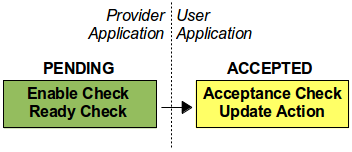
\includegraphics[scale=0.4,keepaspectratio=true]{RepLifecycle.png}
 \caption{Report Lifecycle (Informal Notation)}
 \label{fig:RepLifecycle}
\end{figure}




\subsubsection{Mapping to C-Level Constructs}\label{sec:RepConceptMapping}
The C2 Implementation maps reports to software-level components as follows: out-going reports are mapped to OutComponent components which are implemented in the C module \texttt{CrFwOutCmp} (see section \ref{sec:OutComponent}); incoming reports are mapped to InReport components which are implemented in the C module \texttt{CrFwInRep} (see section \ref{sec:InReport}). Table \ref{tab:RepConceptMapping} shows how the attributes, conditional checks, and actions of reports are mapped to C-level constructs in the C2 Implementation. Note that, in most cases, the mapping depends on whether the report is out-going (i.e. the host application is a provider application) or incoming (i.e. the host application is a user application).

\begin{longtable}{|>{\raggedright}p{2.0cm}|p{11.3cm}|}
\caption{Mapping of Reports to C-Level Constructs} \label{tab:RepConceptMapping}\\
\hline
\rowcolor{light-gray}
\textbf{Name} & \textbf{Mapping to C-Level Construct} \\
\hline\hline
\endfirsthead
\rowcolor{light-gray}
\textbf{Name} & \textbf{Mapping to C-Level Construct} \\
\hline\hline
\endhead
Service Type Attribute & \texttt{ServType} attribute in \texttt{CrFwOutCmp} and \texttt{CrFwInRep} modules. Value set when component is created by its factory and accessible through getter function. \\
\hline
Report Sub-Type Attribute & \texttt{ServSubType} attribute in \texttt{CrFwOutCmp} and \texttt{CrFwInRep} modules. Value set when component is created by its factory and accessible through getter function. \\
\hline
Report Identifier Attribute & \texttt{InstanceId} attribute inherited from base component \texttt{CrFwbaseCmp}. Value set when component is created by its factory and accessible through getter function. \\
\hline
Destination Attribute & \texttt{Dest} attribute in \texttt{CrFwOutCmp}, accessible through getter and setter functions. Attribute not explicitly present in \texttt{CrFwInRep} since the destination of an InReport is, by definition, the host application. \\
\hline
Source Attribute & \texttt{Src} attribute in \texttt{CrFwOutCmp} and \texttt{CrFwInRep} modules. Value set when component is created by its factory and accessible through getter function. \\
\hline
Time Stamp Attribute & \texttt{TimeStamp} attribute in \texttt{CrFwOutCmp} module. Value accessible and controllable through getter and setter functions. Attribute is not present in \texttt{CrFwInRep} module. \\
\hline
Group Attribute & \texttt{Group} attribute in \texttt{CrFwOutCmp} and \texttt{CrFwInRep} modules. Value accessible and controllable through getter and setter functions in the \texttt{CrFwOutCmp} module and in read-only mode through a getter function in the \texttt{CrFwInRep} module.  \\
\hline
Sequence Counter Attribute & \texttt{SeqCnt} attribute in \texttt{CrFwInRep} module. Value set when the component is created by its factory and accessible through getter function. Attribute is not present in \texttt{CrFwOutCmp} module since the sequence counter of out-going reports is set at the time the report is sent out. \\
\hline
Discriminant Attribute & \texttt{Discriminant} attribute in \texttt{CrFwOutCmp} and \texttt{CrFwInRep} modules. Value set when component is created by its factory and accessible through getter function. Update possible through a setter function in \texttt{CrFwOutCmp} module. \\
\hline
Report Parameter Attributes & These attributes are application-specific.  \\
\hline
Enable Check & Function implementing the Enable Check Operation for an out-going report specified through a function pointer in the CR\_FW\_OUTCMP\_INIT\_KIND\_DESC initializer.  \\
\hline
Ready Check & Function implementing the Ready Check Operation for an out-going report specified through a function pointer in the CR\_FW\_OUTCMP\_INIT\_KIND\_DESC initializer. \\
\hline
Repeat Check & Function implementing the Repeat Check Operation for an out-going report specified through a function pointer in the CR\_FW\_OUTCMP\_INIT\_KIND\_DESC initializer.  \\
\hline
Acceptance Check & The part of the acceptance check which verifies validity of the report type and availability of resources is implemented in the Load Command/Report Procedure of the InLoader (see section \ref{sec:InLoader}). The report-specific part of the acceptance check is implemented in the Validity Check Operation specified through a function pointer in the CR\_FW\_INREP\_INIT\_KIND\_DESC initializer.  \\
\hline
Update Action & Function implementing the Update Action Operation for an out-going report specified through a function pointer in the CR\_FW\_OUTCMP\_INIT\_KIND\_DESC initializer. Function implementing the Update Action Operation for an incoming report specified through a function pointer in the CR\_FW\_INREP\_INIT\_KIND\_DESC initializer. \\
\hline
\end{longtable}




%===========================================================================
\section{Packet Interface}\label{sec:PcktInterface}
CORDET applications interact with each other by exchanging commands and reports. Within an application, commands and reports are encapsulated in components but, when they travel from one application to another (over some communication channel which is provided by some middleware external to the applications themselves), they take the form of \textit{packets} (see section \ref{sec:MwLayer}). A report or command packet is an ordered sequence of bytes that contains all the information required to reconstruct a report or command. 

Thus, the interface between two CORDET applications is packet-based. More precisely, an application needs an \textit{out-going interface} through which it can send to another application a packet representing a command or a report and it needs an \textit{incoming interface} through which it can receive from other applications packets representing commands or reports.  

The CORDET Framework assumes that a middleware is present which offers \textit{physical connections} through which two applications can send packets to each other. A physical connection then is a data channel provided by a middleware and capable of transporting packets from one application to another application. 

A CORDET system (namely a set of CORDET applications connected to each other by a middleware) builds a set of \textit{logical connections} on top of the physical connections offered by the middleware. A logical connection allows two applications A1 and A2 to exchange packets either directly through a physical connection linking A1 to A2 (in which case the logical connection coincides with a physical connection) or through a chain of other applications which are linked to each other and to A1 and A2 by physical connections. This is illustrated in figure \ref{fig:PhysicalAndLogicalConnections}. The figure shows a CORDET system consisting of four applications (yellow boxes in the figure). The applications are linked to each other by three physical connections (black lines in the figure). In this system, the following kinds of logical connections might, for instance, be defined:

\begin{enumerate}
\item A logical connection between applications A and B which is built upon physical connection C1;
\item A logical connection between applications B and D which is built upon physical connection C3;
\item A logical connection between applications A and C which is built upon physical connections C1 and C2 and application B acting as re-routing node.
\end{enumerate}

When a packet travels through an application en route to another application, it is said to be \textit{re-routed}. Packet re-routing is a function which is defined by the CORDET Framework and is therefore supported by default by CORDET Systems. In figure \ref{fig:PhysicalAndLogicalConnections} a packet travelling along a logical connection from application A to application C is re-routed by application B.

This section specifies the interfaces through which applications send packets to and receive them from the middleware and it specifies the re-routing logic which allows applications to exchange packets even in the absence of a direct physical connection linking them. 

\begin{figure}[ht]
 \centering
 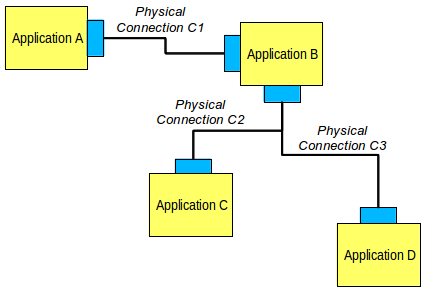
\includegraphics[scale=0.5,keepaspectratio=true]{PhysicalAndLogicalConnections.png}
 \caption{Physical And Logical Connections}
 \label{fig:PhysicalAndLogicalConnections}
\end{figure} 

%---------------------------------------------------------------------------------
\subsection{Middleware Assumptions}\label{sec:MwAssumptions}
Although, the CORDET Framework does not specify the middleware through which applications may exchange packets with each other, it assumes this middleware to satisfy certain, very generic, assumptions. The next two sub-sections define the assumptions made by the CORDET Framework on, respectively, out-going interfaces (interfaces through which packets are sent to another application over a physical connection) and incoming interfaces (interfaces through which packets are received from other applications over a physical connection).

%---------------------------------------------------------------------------------
\subsubsection{Out-Going Interface}\label{sec:OutGoingConnections}

An out-going interface is an interface through which an application sends packets to another application over a physical connection provided by a middleware. The following assumptions are made by the CORDET Framework about out-going connections:

\begin{fw_itemize}
\item[A1]{A connection may be in one of two states: AVAIL or NOT\_AVAIL.}
\item[A2]{If a connection is in state AVAIL, then it is capable of accepting at least one entire packet for eventual transfer to its destination.}
\item[A3]{A connection offers a non-blocking \texttt{Send} operation through which an application can make a request for a packet to be sent to its destination.}
\item[A4]{The \texttt{Send} operation either forwards a packet to its destination (if the middleware is in state AVAIL when the \texttt{Send} request is made) or else it does nothing but notify the caller that the packet cannot be forwarded (if the middleware is in state NOT\_AVAIL when the \texttt{Send} request is made).}
\item[A5]{A connection may make a transition between the AVAIL and NOT\_AVAIL states at any time.}
\item[A6]{A connection may be queried for its current state.}
\end{fw_itemize}

These assumptions correspond to a middleware which accepts packets one at a time and which implements a potentially complex protocol to deliver them to their destination. This protocol may include buffering of packets (to bridge periods of non-availability of the physical link), splitting of packets into smaller messages (to accommodate restrictions on the maximum length of a transmission message), and re-sending of packets which have not been successfully delivered (to ensure continuity of service). 

These protocol complexities manifest themselves at the application level exclusively as transitions between states AVAIL and NOT\_AVAIL (e.g. the middleware connection  becomes unavailable when the middleware buffer is full, or when a packet has to be broken up into messages which have to be sent separately, or when a packet has to be re-sent). Thus, the application is shielded from protocol-level complexity and is only required to be able to handle periods of non-availability of the middleware connection.

Note also that there is no assumption that the middleware be able to signal a change of state of a connection from NOT\_AVAIL to AVAIL. Such a capability could be exploited by an application but is not mandated by the CORDET Framework. Thus, applications are compatible both with a “polling architecture” where the middleware connection is periodically queried for its availability status and with a “call-back architecture” where the application waits to be notified of the middleware's availability. 

%---------------------------------------------------------------------------------
\subsubsection{Incoming Interface}\label{sec:IncomingConnections}

An incoming interface is an interface through which an application receives packets from another application over a physical connection provided by a middleware. The following assumptions are made by the CORDET Framework about incoming connections:

\begin{fw_itemize}
\item[B1]{A connection may be in one of two states: WAITING or PCKT\_AVAIL.}
\item[B2]{If a connection is in state PCKT\_AVAIL, then there is at least one packet that is ready to be collected by the application.}
\item[B3]{A connection offers an operation through which a packet that is waiting to be collected can be collected.}
\item[B4]{A connection may make a transition from state PCKT\_AVAIL to WAITING exclusively as a result of the call to the operation to collect a packet.}
\item[B5]{A connection may make a transition from state WAITING to PCKT\_AVAIL at any time.}
\item[B6]{A connection may be queried for its current state.}
\end{fw_itemize}

These assumptions correspond to a middleware which implements a potentially complex protocol for processing incoming packets. This protocol may include: the defragmentation of packets which are transferred in several messages; the multiplexing of channels from several packet sources; the generation of low-level acknowledgements for incoming packets; the buffering of incoming packets. 

These protocol complexities manifest themselves at the application level exclusively as transitions between state PCKT\_AVAIL and WAITING (e.g. the middleware connection  is in state WAITING when no packet has arrived, or when messages are being spliced together to compose a complete packet, or when an acknowledgement is being generated). Thus, the application is shielded from protocol-level complexity and is only required to be able to handle periods when no incoming packet is present.

Note also that there is no assumption that the middleware be able to signal a change of state of a connection from WAITING to PCKT\_AVAIL. Such a capability, if it exists, can be exploited by an application but is not mandated by the CORDET Framework. Thus, an application is compatible both with a “polling architecture” where the middleware connection is periodically queried for the presence of incoming packets and with a “call-back architecture” where the application waits to be notified of the arrival of a packet. 
 

%---------------------------------------------------------------------------------
\subsection{Packet Implementation}\label{sec:PcktImpl}

At implementation level, a packet is an array of bytes. The C2 Implementation pre-defines type \texttt{CrFwPckt\_t} to represent packets.

The layout of packets is entirely defined at application level. The C2 Implementation specifies an interface (in header file \texttt{CrFwPckt.h}) through which a new packet can be created and its various fields can be accessed. 

Packet creation is managed through two functions (\texttt{CrFwPcktMake} and \texttt{CrFwPcktRelease}) which can be used to, respectively, create and release a packet. The creation function takes as an argument the length of the packet. Function \texttt{CrFwPcktIsAvail} can be used to query the interface for the availability of a packet of a given length. The implementation of these functions is left open. In the simple case of an application developer who is not concerned about dynamic memory allocation, these functions can be implemented simply as wrappers for \texttt{malloc} and \texttt{free}. Other users who wish to avoid dynamic memory allocation operations at run-time must implement their own memory management scheme.

For each command or report attribute, the packet interface \texttt{CrFwPckt.h} specifies a function to read and write the value of the attribute. The implementation of these functions depends on the way the attributes of commands and reports are encoded in a packet. The implementation of these functions (i.e. the body file \texttt{CrFwPckt.c}) must therefore be provided by application developers. A stub implementation, which is used in the Test Suite of the C2 Implementation, is provided in the configuration directory \texttt{/cr/src/CrConfigTestSuite}.

Since the framework provides one single interface for decoding and encoding packets, the simplest option for application developers is to use the same layout for all packets used by the application, irrespective of their type or of their destination or source. If this is not possible, then the getter and setter functions of interface \texttt{CrFwPckt.h} must implement logic which makes their outcome dependent on the content of the packet itself. Thus, for instance, if different packet sources use different layouts, the getter functions will have to inspect the source of a packet before deciding how to decode the value of a packet's attribute. In the case of the setter functions, this approach requires that the order in which the packet attributes are set be specified. The only place in the CORDET Framework where packets are configured is the function to create a new OutComponent (\texttt{CrFwOutFactoryMakeOutCmp}). This function accordingly guarantees the order in which the packet attribute are set (the order is: packet report/command flag (which determines whether the packet holds a report or a command), packet source (i.e. the host application), packet group, packet type, packet sub-type, and packet discriminant).

%---------------------------------------------------------------------------------
\subsection{Packet Interface Management}

The packet interface concept for CORDET applications is illustrated in figure \ref{fig:PcktInterfaceConcept} using an information notation.

The management of the out-going packet interface is performed by one or more OutStream components. An OutStream component encapsulates an out-going interface through which packets are sent to a certain destination. An application has one OutStream component for each destination to which it may send packets.

The management of the incoming packet interface is performed by an InStream component. An InStream component encapsulates the incoming interface through which an application receives packets from a certain packet source. An application has one InStream component for each source from which it may receive packets.

Packets which are received by an InStream in application A and which have application A as their destination are made available to the internal components of application A. Packets which are received by an InStream in application A and which have an application other than A as their destination are instead re-routed. This means that they are handed over to an OutStream for forwarding to another application (either their final destination or another intermediate application on the way to their final destination).

As an example, consider again the CORDET System of figure \ref{fig:PhysicalAndLogicalConnections} and consider first the case of a packet which is sent by application A to application B over connection C1. This packet is placed on connection C1 by an OutStream in application A and is received by an InStream in application B. Since the destination of the packet is application B itself, the InStream makes the packet available to the internal components of application B.

Consider next the case of a packet which is sent by application A to application C and which must therefore be re-routed by application B. This packet is initially placed on connection C1 by an OutStream in application A and is received by an InStream in application B. This InStream recognizes that the packet destination is not B and therefore re-routes it by directly handing it over to an OutStream which places it on connection C2. At the other end of this connection, the packet is received by an InStream in application C which recognizes that the packet has arrived at its final destination and therefore makes it available to the internal components of application C. 

\begin{figure}[ht]
 \centering
 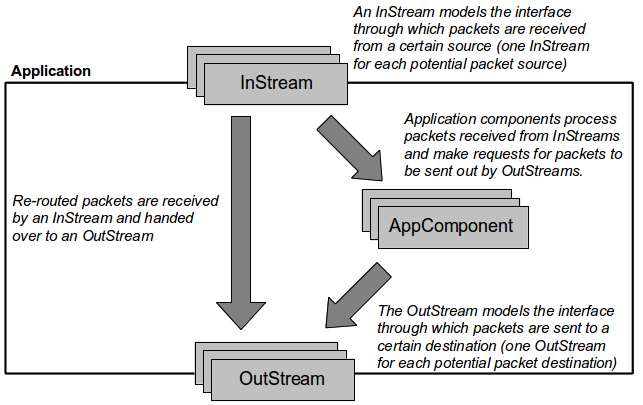
\includegraphics[scale=0.45,keepaspectratio=true]{PcktInterfaceConcept.png}
 \caption{Packet Interface Concept}
 \label{fig:PcktInterfaceConcept}
\end{figure}


%---------------------------------------------------------------------------------
\subsubsection{The OutStream Component}\label{sec:OutStream}
This component models the out-going interface through which packets representing either commands (in a service user application) or reports (in a service provider application) are sent to their destination. The OutStream is therefore located at the interface between an application and the middleware layer. 

An application A may send packets to several destinations. The packets may either originate within application A itself or they may have originated in some other application (the latter is the case if application A is re-routing the packets). Depending on the characteristics of the middleware, only one OutStream component may be present in application A with the multiplexing of the out-going connections to the packet destinations being done in the middleware, or several OutStream components may be present each handling packets to a subset of destinations. If an application is sending internally generated packets to a certain destination D and is also re-routing packets to the same destination D, then it must use the same OutStream for both kinds of packets. 

The OutStreams are responsible for assigning the sequence counter attributes of out-going packets generated by an application. Since sequence counters are incremented according to a packet's group, all packets belonging to the same group must go through the same OutStream.

The OutStream component extends the Base Component of section \ref{sec:BaseCmp} and it therefore inherits the initialization and configuration logic defined by the Base Component. In the initialization and configuration process, the OutStream is linked to the middleware. This process is necessarily application-specific (because the middleware is not specified by the CORDET Framework). However, the CORDET Framework specifies that an OutStream component may only become configured (i.e. it may enter state CONFIGURED) after the middleware connection has become available (it has entered state AVAIL). This ensures that an OutStream only becomes configured after its middleware connection has terminated its own initialization and configuration process.

\begin{figure}[ht]
 \centering
 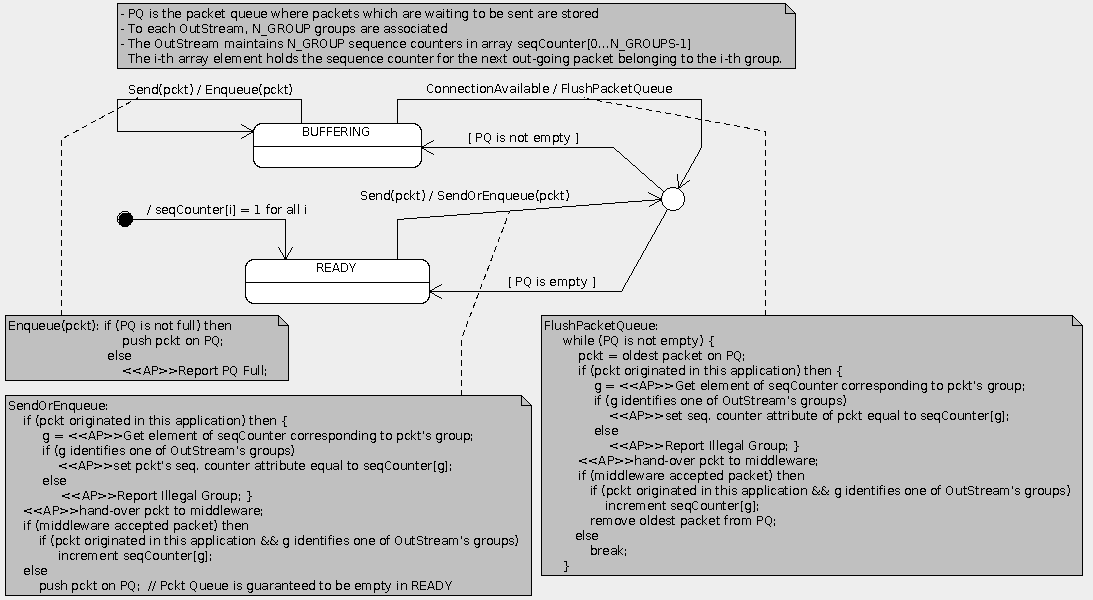
\includegraphics[scale=0.35,keepaspectratio=true]{OutStream.png}
 \caption{The OutStream State Machine}
 \label{fig:OutStream}
\end{figure}

In state CONFIGURED, the behaviour of an OutStream is described by the state machine of figure \ref{fig:OutStream} (the \textit{OutStream State Machine}). The state machine has two states: READY and BUFFERING. State READY represents a situation where the connection is expected to be available and the OutStream hands over packets to the middleware. State BUFFERING represents a situation where the connection may be unavailable and where packets are buffered without being handed over to the middleware.

The OutStream State Machine reacts to two commands: \texttt{Send} and \texttt{ConnectionAvailable}. Command \texttt{Send} is issued by the host application when it wishes to send a packet to its destination. If, at the time a \texttt{Send} request is made, the state machine is in state BUFFERING, then the packet is enqueued in the \textit{Packet Queue}. 

The Packet Queue is an internal data structure where packets which are waiting to be sent are stored. The size of the packet queue is fixed and is defined as part of the OutStream configuration. Attempts to enqueue a packet in a full queue are reported as errors.

The Packet Queue is a FIFO queue. This guarantees that the OutStream component delivers packets to the middleware in the same order in which it receives them from its host application. 

If, instead, a \texttt{Send} request is made at a time when the OutStream is in state READY, then an attempt is made to hand over the packet to the middleware. If this succeeds, the OutStream remains in state READY. If instead the hand-over to the middleware fails, the packet is enqueued and the OutStream makes a transition to state BUFFERING. Note that the logic of the OutStream State Machine guarantees that, at entry into state READY, the packet queue is empty.
 
The \texttt{Send} command may either fail or succeed. If it results in its packet being enqueued on the Packet Queue, then the \texttt{Send} command succeeds (note that property P3 below ensures that a packet which has been enqueued will eventually be handed over to the middleware). If instead it results in its packet being lost because, at the time the \texttt{Send} command was called, the Packet Queue was full, then the \texttt{Send} command fails. 

Command \texttt{ConnectionAvailable} would typically be generated by the middleware when the connection (or one of the connections) associated to the OutStream changes from NOT\_AVAIL to AVAIL. This command is used to trigger the flushing of the Packet Queue. When the OutStream receives command \texttt{ConnectionAvailable} it empties the Packet Queue one packet at a time until the queue is empty or the connection becomes unavailable.

The out-going packets which are handled by an OutStream may have two origins: (a) they may have originated in the same application to which the OutStream belongs, or (b) they may be re-routed packets which originate from some other application and which are using the OutStream's application as a gateway on the way to their destination (see figure \ref{fig:PcktInterfaceConcept}). In case (a), the OutStream is responsible for setting the sequence counter attribute of the out-going packet. In case (b), by contrast, the packet's sequence counter attribute is already set (it has been set by the application where the packet originated).

In case (a), the sequence counter is incremented according to the group to which an out-going command or report belongs. Thus, an OutStream maintains an array of sequence counters, one for each group to which its out-going commands or reports may belong. The i-th element of this array holds the value of sequence counter which will be assigned by the OutStream to the next out-going command or report belonging to the i-th group managed by the OutStream. The sequence counters are initialized to 1 when the OutStream is reset (i.e. the first value of sequence counter assigned to an out-going command or report after the OutStream is reset is 1). If a command or report has an illegal group attribute, this is reported as an error.

The OutStream is responsible for computing and setting the CRC of an out-going packet. This can only be done after the sequence counter has been set (because the sequence counter itself contributes to the value of the CRC).
 


The C2 Implementation implements the OutStream component in module \texttt{CrFwOutStream}. 


%---------------------------------------------------------------------------------
\subsubsection{The OutStreamRegistry Component}\label{sec:OutStreamRegistry}
As discussed in section \ref{sec:OutStream}, for each command or report destination, one OutStream component must be instantiated by an application. The CORDET Framework accordingly defines an OutStreamRegistry component which encapsulates the link between the command and report destinations and the associated OutStream.  

Only one operation is defined at framework level for the OutStreamRegistry. The \texttt{OutStreamGet} operation lets a user retrieve the OutStream corresponding to a certain command or report destination. The command or report destination is identified by the value of the destination attribute of the command or report (see sections \ref{sec:CmdAttributes} and \ref{sec:RepAttributes}). 

If an invalid destination is provided to the \texttt{OutStreamGet} operation, nothing is returned by the operation itself but this is not treated as an error by the OutStreamRegistry component. If the use of an invalid destination represents an error, this must be handled by the user of the OutStreamRegistry.

Since the range of potential command and report destinations is unknown at framework level, the \texttt{OutStreamGet} operation is an adaptation point for the OutStreamRegistry. The link between the command and report destinations and their OutStreams is a configuration parameter for the OutStreamRegistry. 

Only one instance of the OutStreamRegistry should exist in an application. 

The OutStreamRegistry is defined as an extension of the Base Component.


In the C2 Implementation, the OutStreamRegistry component is merged with the OutStream component and is therefore implemented in module \texttt{../cordetfw/CrFwOutStream} (i.e. it is implemented in the same module which implements the OutStream component). This module, in addition to defining the functions implementing the OutStream operations, also defines function \texttt{CrFwOutStreamGet} to implement the \texttt{OutStreamGet} operation. 


%---------------------------------------------------------------------------------
\subsubsection{The InStream Component}\label{sec:InStream}
The InStream component models the interface through which packets representing incoming commands or reports are received by an application. The InStream component is therefore located at the interface between an application and the middleware layer (see section \ref{sec:MwLayer}). 

An application A may receive packets from several sources. The packets may either have application A as their destination or they may be intended for some other application. In the latter case, application A is responsible for re-routing the packets. Depending on the characteristics of the middleware, only one InStream component may be present in application A with the multiplexing of the incoming connections from the packet sources being done in the middleware, or several InStream components may be present each handling packets from a subset of incoming connections. 

Although several connections may be managed by the same InStream, a connection can only send its packet to one InStream (i.e. a situation where the same connection is controlled by several InStreams and several InStreams are therefore handling packets from the same source is not allowed).

The InStreams are responsible for checking the sequence counter attributes of incoming packets received by an application. Since sequence counters are incremented according to a packet's group, all packets belonging to the same group must arrive through the same InStream.

The InStream component is defined as an extension of the Base Component of section \ref{sec:BaseCmp} and it therefore inherits the initialization and configuration logic defined by the Base Component. In the initialization and configuration process, the InStream is linked to the middleware. This process is therefore necessarily application-specific (because the middleware is not specified by the CORDET Framework). However, the CORDET Framework specifies that an InStream component may only become configured (i.e. it may enter state CONFIGURED) after the middleware connection has terminated its own initialization and configuration. This ensures that an InStream only becomes configured after its middleware connection has terminated its own initialization and configuration process.

\begin{figure}[ht]
 \centering
 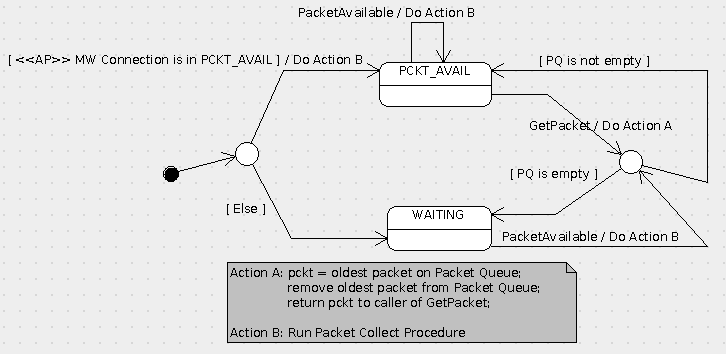
\includegraphics[scale=0.35,keepaspectratio=true]{InStream.png}
 \caption{The InStream State Machine}
 \label{fig:InStream}
\end{figure}

\begin{figure}[h]
 \centering
 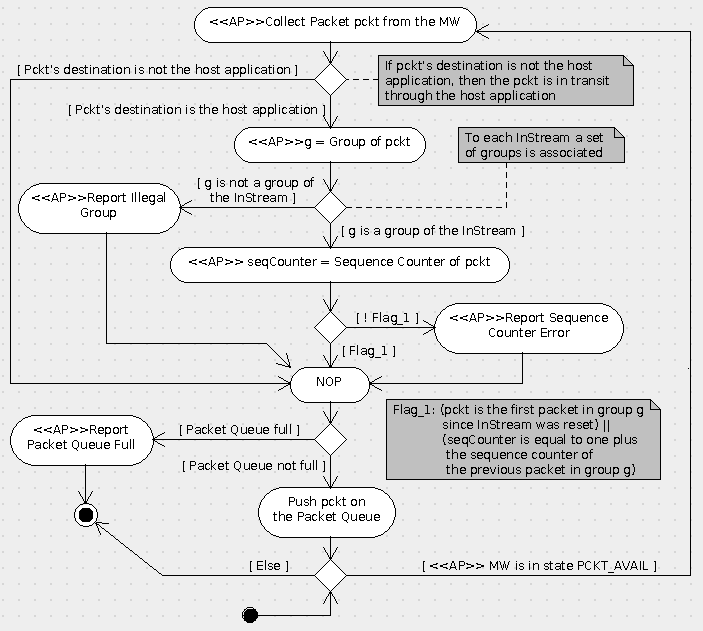
\includegraphics[scale=0.35,keepaspectratio=true]{PacketCollect.png}
 \caption{The Packet Collect Procedure}
 \label{fig:PacketCollect}
\end{figure}

In state CONFIGURED, the behaviour of an InStream is described by the state machine of figure \ref{fig:InStream} (the \textit{InStream State Machine}). The state machine has two states: WAITING and PCKT\_AVAIL. State WAITING represents a situation where no incoming packets are waiting to be collected by the host application. State PCKT\_AVAIL represents a situation where at least one incoming packet has been collected from the middleware and is now waiting to be collected by the host application. 

The InStream component stores packets it has collected from the middleware in the \textit{Packet Queue}. The Packet Queue is an internal InStream data structure where packets which have been collected from the middleware are stored and where they remain available until the application retrieves them. The size of the packet queue is fixed and is defined as part of the InStream configuration. Attempts to enqueue a packet in a full queue are reported as errors.

The Packet Queue is a FIFO queue. This guarantees that the InStream component delivers packets to its host application in the same order in which it has collected them from the middleware. The InStream State Machine reacts to two commands: \texttt{GetPacket} and \texttt{PacketAvailable}. Command \texttt{GetPacket} is issued by the host application when it wishes to collect an incoming packet. If the command is received when the state machine is in state PCKT\_AVAIL (namely when at least one packet is available in the Packet Queue), then the command results in the oldest packet in the Packet Queue being returned to the caller. If the packet thus returned is the last on the queue, the command triggers a transition to state WAITING. 

If the \texttt{GetPacket} command is received when the state machine is in state WAITING, the command has no effect and returns nothing.

Command \texttt{PacketAvailable} would typically be issued under two conditions: (a) in response to the middleware connection changing from NOT\_AVAIL to AVAIL, or (b) periodically to check whether any packets are available at the middleware interface. Case (a) corresponds to a call-back architecture where the middleware alerts the application that a new packet has arrived. Case (b) corresponds to a polling architecture where the application periodically checks whether a new packet has arrived. 

Reception of command \texttt{PacketAvailable} causes the \textit{Packet Collect Procedure} of figure \ref{fig:PacketCollect} to be run. This procedure collects all packets currently available at the middleware. The packets are stored in the InStream's Packet Queue. 

Also as part of the processing of the \texttt{PacketAvailable} command, the \textit{Packet Collect Procedure} checks the sequence counter attribute of incoming packets which have the host application as their destination. To each InStream, a set of groups are associated. For each group, the InStream maintains a sequence counter. When a packet is received which belongs to that group, the InStream checks that its sequence counter has incremented by one with respect to the previous packet in the same group. If the procedure finds that the sequence counter has not incremented by one, it reports the sequence counter error. An error is also reported if the group attribute of an incoming packet does not correspond to one of the groups managed by the InStream.

The sequence counter check is only done for packets which have the host application as their destinations. Packets which are in transit (i.e. packets which must be re-routed to some other application) do not undergo any check on their sequence counter. This logic ensures that the sequence counter check is only performed once by the InStream that receives a packet in the destination application of that packet. 


The C2 Implementation implements the InStream component in module \texttt{CrFwInStream}. This implementation follows the specification of the CORDET Framework with one restriction: an InStream component can only handle packets from one single packet source. Thus, an application must instantiate one InStream for each source from which it may receive packets. More precisely, the rules for deciding the number of InStreams in an application are as follows:

\begin{itemize}
\item[R1]{If an application receives packets from source S1, then it must have a dedicated InStream for source S1.}
\item[R2]{If an application re-routes packets from source S2 to other destinations, then it must have a dedicated InStream for source S2.}
\item[R3]{If an application receives packets from a source S and also re-routes packets from the same source S, then it must use the same InStream for both kinds of packets.}
\end{itemize}

Thus, for each command or report source, one (and only one) InStream component must be instantiated by an application. Function \texttt{CrFwInStreamGet} lets a user retrieve the InStream corresponding to a certain command or report source. 

If an invalid source is provided to the \texttt{CrFwInStreamGet} operation, nothing is returned by the operation itself but this is not treated as an error by the \texttt{CrFwInStreamGet} operation. If the use of an invalid packet source represents an error, this must be handled by the caller of \texttt{CrFwInStreamGet}.

The collection of packets from the middleware is mediated by two functions which implement two framework adaptation points: function \texttt{CrFwPcktCollect\_t} implements the Packet Collection Operation and function CrFwPcktAvailCheck\_t implements the Packet Available Check Operation. 

The Packet Collect Operation (function \texttt{CrFwPcktCollect\_t}) collects a packet from the middleware. Its return value is a packet in the sense of section \ref{sec:PcktImpl}. The Packet Collect Operation must therefore create the packet it returns using the \texttt{CrFwPcktMake} function. Hence, the Packet Collect Operation only returns a packet if a command or report has arrived at the middleware and if function \texttt{CrFwPcktMake} is capable of returning an empty packet where the newly arrived command or report can be stored. 

The Packet Available Check Operation (function \texttt{CrFwPcktAvailCheck\_t}) can be used to query the middleware for the availability of a packet to be collected. More precisely, if this operation returns: 'a packet is available', then a call to the Packet Collect Operation will return a non-NULL packet. Note that this means that the Packet Available Check Operation must perform a double check: it must check whether a command or report has been received by the middleware and it must verify whether the \texttt{CrFwPcktMake} function would be able to return a packet capable of holding the newly arrived command or report. The latter check can be done with function \texttt{CrFwPcktIsAvail}.


%=============================================================================================
\section{Command and Report Management}\label{sec:CmdAndRepManagement}
This section describes the mechanisms which the CORDET framework makes available for the management of commands and reports in a CORDET application. These mechanisms are entirely independent of the concrete actions and checks attached to a specific command or report. It is precisely this independent that makes it possible for the framework to provide generic report and command handling components which can be reused by applications.

This section introduces the components which are responsible for the management of commands and reports and describes their interrelationships. The following sections describe each kind of component in greater detail with the exception of the InStream and OutStream components which are already covered in sections \ref{sec:InStream} and \ref{sec:OutStream} and of the factory components which are already covered in section \ref{sec:CmpImpl}.

%---------------------------------------------------------------------------------
\subsection{Management of Out-Going Commands and Reports}\label{sec:ManagementOfOutGoingCmdAndRep}
\textit{Out-going commands} are commands in a user application (namely in an application which sends commands to a service provider) and \textit{out-going reports} are reports in a provider application (namely in an application which sends reports to a service user).

Out-going commands and out-going reports are treated together because their management is performed in the same way and is based on the following components:

\begin{itemize}
\item \textbf{OutComponent}
This component models the generic behaviour of an out-going command or report. Concrete commands or report generated by an application are defined as extensions of the base OutComponent component. 
\item \textbf{OutFactory}
This is a component factory (in the sense of section \ref{sec:CmpInst}) which provides unconfigured instances of OutComponents to encapsulate out-going commands or reports.
\item \textbf{OutLoader}
After an application has configured an OutComponent representing an out-going command or report, it loads it into the OutLoader. This component is responsible for selecting the appropriate OutManager to process the out-going command or report. 
\item \textbf{OutManager}
This component is responsible for controlling an out-going command or report until the OutComponent which encapsulates it is serialized to the OutStream and sent to its destination as a packet.
\item \textbf{OutStream}
This component models the interface through which out-going commands and reports are sent to their destination.
\item \textbf{OutRegistry}
This component acts as a registry for pending OutComponents. It provides information about the state of the OutComponent to other parts of the host applications. 
\end{itemize}

Note that the OutFactory, OutLoader, and OutRegistry components are singletons and it is therefore assumed that only one instance of each exists in an application. It is also assumed that there is one (and only one) OutStream for each destination to which commands may be sent (see usage constraints at the end of section \ref{sec:OutStream}).

\begin{figure}[h]
 \centering
 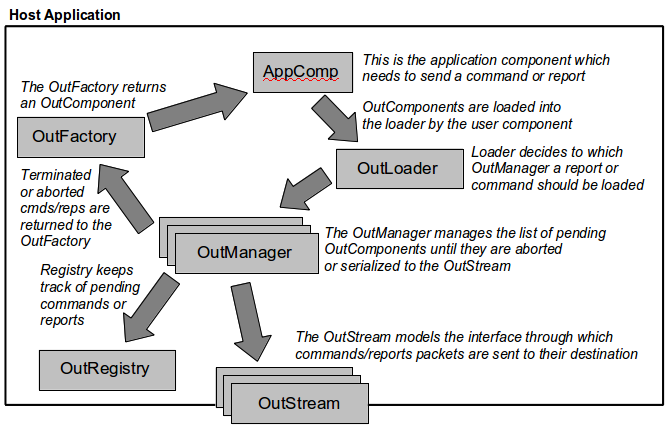
\includegraphics[scale=0.50,keepaspectratio=true]{OutGoingCmdAndRep.png}
 \caption{Management of Out-Going Commands and Reports}
 \label{fig:OutGoingCmdAndRep}
\end{figure}

The lifecycle of an out-going report or command is shown in figure \ref{fig:OutGoingCmdAndRep} using and informal notation and can be summarized as follows:
\begin{enumerate}
\item When the host application decides that it must issue a command or a report, it asks the OutFactory for an unconfigured OutComponent instance to encapsulate the out-going command or report.
\item The application configures the OutComponent and then loads it in the OutLoader.
\item The OutLoader selects an OutManager and loads the OutComponent into it. The selection of the OutManager will often be based on the urgency with which the command or report must be issued (e.g. each OutManager component is characterized by a certain priority level). 
\item\label{lst:OutComponentProcessing} The OutManager component processes the out-going command or report. If the command or report is disabled, it is aborted and the component which encapsulated it is returned to its factory (where it is either destroyed or is reused). If instead the command or report is enabled, it remains pending in the OutManager until its ready check indicates that the conditions are in place for it to be issued. 
\item The report or command is issued by serializing its OutComponent to a packet which is then handed over to the OutStream. The OutStream is responsible for sending the packet to its destination. 
\item After the OutComponent has been serialized and sent to its destination, the OutManager evaluares the outcome of its Repeat Check. If this is equal to "repeat", the content of the OutComponent is updated and the OutComponent is then processed again as per point \ref{lst:OutComponentProcessing} above. If instead the repeat check had returned "no repeat", processing of the OutComponent terminates and the OutComponent is returned to its factory.
\end{enumerate}




The C2 Implementation provides implementations for each of the CORDET components discussed above. Table \ref{tab:CmpList} shows the mapping to the C-modules which implement them.

%---------------------------------------------------------------------------------
\subsection{Management of Incoming Commands and Reports}\label{sec:ManagementOfIncomingCmdAndRep}
\textit{Incoming commands} are commands in a provider application (namely in an application which receives commands from a service user) and \textit{incoming reports} are reports in a user application (namely in an application which receives reports from a service provider).

Incoming commands and incoming reports are treated together because their management is performed in a similar way. 

The management model specified by the framework for incoming commands and reports is based on the definition of the following components:
\begin{itemize}
\item \textbf{InCommand} 
This component models the generic behaviour of a command on a provider application (namely of an incoming command). Concrete incoming commands are defined as extensions of the base InCommand component.
\item \textbf{InReport}
This component models the generic behaviour of a report on a user application (namely of an incoming report). Concrete incoming reports are defined as extensions of the base InReport component.
\item \textbf{InStream}
This component models the interface through which incoming commands and reports are received by an application. 
\item \textbf{InFactory}
The InStream delivers an incoming command or incoming report as a packet consisting of a stream of bytes which must be deserialized to create an InCommand or InReport instance to represent it. The InFactory component encapsulates the component instance creation process.
\item \textbf{InLoader}
This component is responsible for retrieving packets which become available at the InStreams. The InLoader may either forward an incoming packet (if its destination is not the host application), or it may process it as an incoming report (if the packet holds a report), or it may process it as an incoming command (if the packet holds a command). The processing of incoming commands or reports is as follows. The InLoader deserializes the packet and creates an InCommand or InReport instance to represent it and then loads it into an InManager. The InManager will be responsible for executing the InCommand or InReport.
\item \textbf{InManager}
This component controls the execution of an incoming command or incoming report until all its actions have been completed.
\item \textbf{InRegistry}
This component acts as a registry for pending InCommand and InReport. It can provide information about their state to other parts of the applications.  
\end{itemize}

Note that InFactory, InLoader, InRegistry and InStream are singletons and it is
therefore assumed that only one instance of each exists in an application. 

\begin{figure}[h]
 \centering
 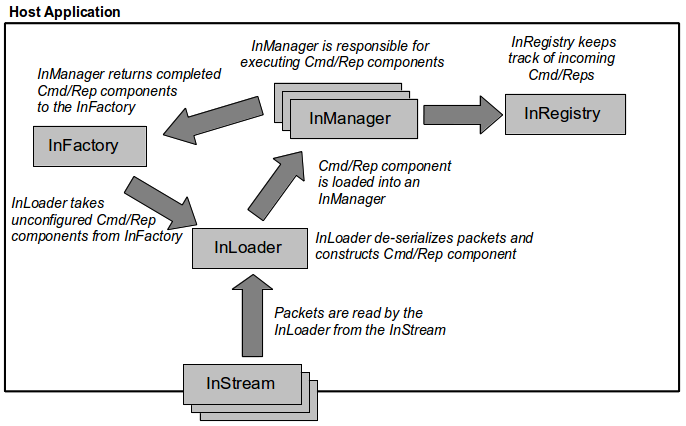
\includegraphics[scale=0.5,keepaspectratio=true]{IncomingCmdAndRep.png}
 \caption{The Management of Incoming Commands and Reports}
 \label{fig:IncomingCmdAndRep}
\end{figure}

The process through which an application processes an incoming command or incoming report is shown using an information notation in figure \ref{fig:IncomingCmdAndRep} and can be summarized as follows:
\begin{enumerate}
\item The InStreams receive packets from other applications. The packets are collected from the InStreams by the InLoader.
\item The InLoader checks the destination of the packet. If it is the host application itself (namely the application within which the InLoader is running), it processes the packet as described below. If it is another application, the InLoader forwards the packet to another application (either its eventual destination or a routing application on the way to its eventual application).
\item An incoming packet may represent either a command or a report. The InLoader identifies the type of the command or report and asks the InFactory to provide an instance of an InCommand (if the packet represents a command) or of an InReport (if the packet represents a report) of that type. 
\item The InCommand or InReport are initially unconfigured. They are configured by deserializing the packet representing the incoming command or incoming report. Henceforth the incoming command or report is represented by the configured InCommand or InReport instance. 
\item The InLoader loads the command or report into an InManager. The InManager is responsible for executing the command or report. In the case of incoming commands, this may require several execution cycles. In the case of incoming reports, at most one execution cycle is sufficient. Depending on the outcome of the conditional checks associated to the incoming command or report, execution may result either in a normal termination or in the command or report being aborted.
\item When the command or report has terminated execution or has been aborted, the InManager returns the InCommand or InReport component instance that held it to the InFactory.
\item The InRegistry is notified of the arrival of incoming commands and reports and of changes of their state. The Inregistry makes this information available to other parts of the host application.
\end{enumerate}



The C2 Implementation provides implementations for each of the CORDET components discussed above. Table \ref{tab:CmpList} shows the mapping to the C-modules which implement them.


%=================================================================================
\section{The OutComponent Component}\label{sec:OutComponent}
The OutComponent component encapsulates an out-going command or an out-going report. This component enforces the generic behaviour that is common to all out-going commands and reports irrespective of their type and it provides access to their attributes.

The OutComponent component – like all other CORDET Framework components – is an extension of the Base Component of section \ref{sec:BaseCmp}. Behaviour which is specific to the OutComponent component is defined by the state machine shown in figure \ref{fig:OutComponent} (the \textit{OutComponent State Machine}). This state machine is embedded within the CONFIGURED state of the Base State Machine. 

\begin{figure}[h]
 \centering
 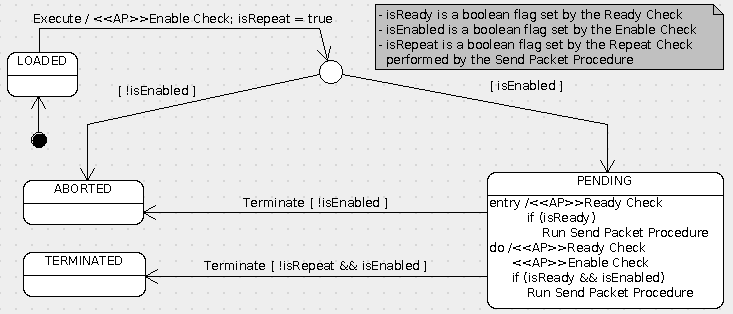
\includegraphics[scale=0.4,keepaspectratio=true]{OutComponent.png}
 \caption{The OutComponent State Machine}
 \label{fig:OutComponent}
\end{figure}

When the OutComponent is retrieved from its factory, it is initialized and reset (depending on the implementation, the \texttt{Reset} command may be issued either by the factory itself or by the user application). After the OutComponent has been successfully reset, the OutComponent State Machine is in state LOADED. The component then waits for the \texttt{Execute} and \texttt{Terminate} commands which are sent to it by its OutManager (see section \ref{sec:OutManager}). 

The OutComponent behaviour depends on the outcome of three checks. The \textit{Enable Check} verifies whether the command or report it encapsulates is enabled or not. If it is enabled, the check sets flag \texttt{isEnabled} to true; if it is disabled, it sets flag \texttt{isEnabled} to false. The \textit{Ready Check} verifies whether the command or report is ready to be sent to its destination. If it is ready to be sent, the check sets flag \texttt{isReady} to true; otherwise it sets the flag to false. The \textit{Repeat Check} verifies whether the command or report should remain pending after being sent to its destination. If the outcome of the Repeat Check is 'Repeat' (i.e. if the OutComponent should be sent to its destination again), flag \texttt{isRepeat} is set to true; if the outcome is 'No Repeat' (i.e. if the OutComponent should not bet sent again to its destination), flag \texttt{isRepeat} is set to false. The three check operations are adaptation points.

At each execution, the OutComponent performs the Enable Check and if this declares the OutComponent to be disabled, it makes a transition to state ABORTED. This marks the end of the OutComponent's lifecycle.

At each execution, the OutComponent has a chance to be sent to its destination. This is done when the OutComponent is declared to be both ready and enabled by its Ready Check and Enable Check. 

The sending operation is performed by the Send Packet Procedure of figure \ref{fig:SendPacket}. The Send Packet Procedure starts by performing the Update Action. Through this action, the OutComponent acquires the information it must transfer to its destination. By default, this action sets the time stamp attribute of the OutComponent. Applications may want to extend this action to load the values of the OutComponent parameters. For this reason, the Update Action is an adaptation point of the OutComponent.

The Send Packet Procedure then retrieves the destination of the OutComponent and then interrogates the OutStreamRegistry to obtain the corresponding OutStream (recall that, in an application, there is one instance of OutStream for each command or report destination). If an OutStream can be found (i.e. if the OutComponent's destination is valid), the procedure serializes the OutComponent to generate a packet which is then handed over to the OutStream. This ensures that the command or report will eventually be sent to its destination. The serialization process is an adaptation point. 

After serializing and handing over the OutComponent to its OutStream, the Send Packet Procedure performs the Repeat Check. This determines whether the OutComponent should be sent to its destination once more (the Repeat Check sets flag \texttt{isRepeat} to true) or whether its life is terminated (the Repeat Check sets flag \texttt{isRepeat} to true). In the latter case, the OutComponent will make a transition to TERMINATED.

If the OutStreamRegistry does not return any OutStream, then the procedure concludes that the OutComponent's destination is invalid and it reports the fact. In this case, the outcome of the Repeat Check is also forced to 'No Repeat' (i.e. flag \texttt{isRepeat} is set to false). 

\begin{figure}[h]
 \centering
 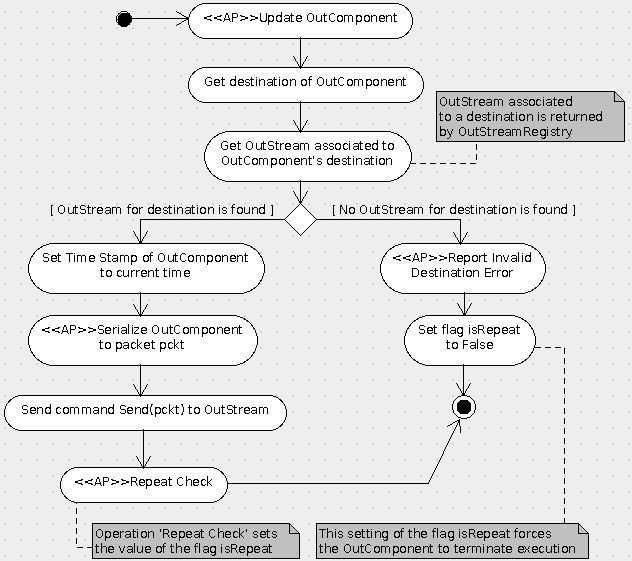
\includegraphics[scale=0.4,keepaspectratio=true]{SendPacket.png}
 \caption{The Send Packet Procedure}
 \label{fig:SendPacket}
\end{figure}

The OutComponent provides visibility over its internal state but it does not provide automatic notifications in case of changes in its internal state. The OutComponent provides access to the attributes of the command or report it encapsulates but it only predefines dummy values for them. The set and value of command or report attributes is therefore an adaptation point for the OutComponent. 

The default implementation of the Enable Check uses one of the services provided by the OutRegistry to determine the enable status of a command or report (see section \ref{sec:OutRegistry}).
 

The C2 Implementation implements the OutComponent component in module \texttt{CrFwOutComponent}. Its adaptation points are defined in \texttt{CrFwOutFactoryUserPar.h}. This header file allows the application developer to define the kinds of OutComponents which must be supported by the application and to define, for each kind of OutComponent, the functions which implement their Ready Check, their Enable Check, and their Serialization operation. The "kind" of OutComponent is identified by the triplet: [service type, command/report sub-type, discriminant value]. 

OutComponents are instantiated dynamically by an application when it needs to generate an out-going command or report. The instantiation is done by means of a \texttt{make} function provided by the OutFactory. The argument to the \texttt{make} function is the OutComponent kind. The release of the OutComponent is done by the framework at the time the OutComponent is handed over to the OutStream.

%=================================================================================
\section{The OutLoader Component}\label{sec:OutLoader}
After a user application has obtained an OutComponent component from an OutFactory, it loads it into the OutLoader. This component is responsible for selecting the appropriate OutManager to process the out-going command or report.

For this purpose, the OutLoader maintains a list of OutManagers (the List of OutManagers or LOM). The LOM holds all the OutManagers which have been instantiated in an application. 

The OutLoader component offers one operation – the \texttt{Load} operation – to load an OutComponent into an OutManager. When this operation is called, the OutLoader decides to which OutManager in the LOM to load an OutComponent. The policy for selecting the OutManager in the LOM is an adaptation point. After the OutComponent is loaded into the selected OutManager, the procedure may activate the selected OutManager (i.e. it may release the thread which is controlling the execution of the selected OutManager). This is useful where there is a need to process the out-going command or report as soon as it is loaded into the OutLoader (normally, the command or report would only be processed when the OutManager is executed). 
 
The \texttt{Load} operation is modelled by the procedure shown in figure \ref{fig:OutLoaderLoad}. A call to operation \texttt{Load} causes this procedure to be started and executed. The procedure executes in one single cycle and therefore terminates as part of the call to operation \texttt{Load}. 

No facilities are defined for dynamically changing the set of OutManagers in the LOM. Changes in the list of OutManagers can only be done by reconfiguring and then resetting the OutLoader component.

\begin{figure}[h]
 \centering
 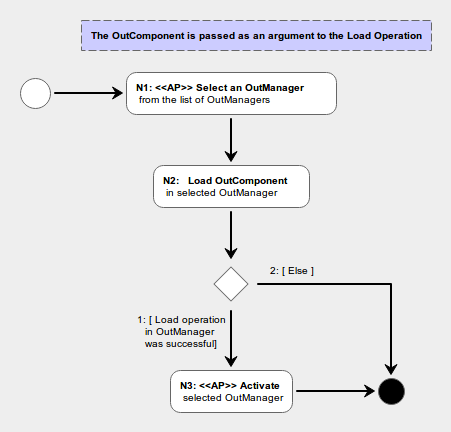
\includegraphics[scale=0.45,keepaspectratio=true]{OutLoaderLoad.png}
 \caption{The OutLoader Load Procedure}
 \label{fig:OutLoaderLoad}
\end{figure}


The C2 Implementation implements the OutLoader component in module \texttt{CrFwOutLoader}. Its adaptation points are defined in \texttt{CrFwOutLoaderUserPar.h}. In most cases, the only adaptation point for which a non-default implementation is required is the one covering the definition of the function which selects the OutManager where an out-going command or report should be loaded. 

By default, the initialization, reset and shutdown operations of the OutLoader are the same as on the Base Component but these operations are implemented as adaptation points so that the user has a chance to use them to initialize or reset the data structures which are used to control the selection of the OutManager where an out-going command or report is loaded.

%=================================================================================
\section{The OutManager Component}\label{sec:OutManager}
This component is responsible for maintaining a list of pending OutComponents and for repeatedly executing them until they are serialized and sent to their destination.
The list of pending commands is called the \textit{Pending OutComponent List} or POCL. The POCL has a fixed size which is defined when the OutManager is initialized. 

The OutManager component offers a \texttt{Load} operation through which an OutComponent can be added to the POCL (see activity diagram in figure \ref{fig:OutManagerLoad}). This operation is called by the OutLoader of the previous section. The \texttt{Load} operation may fail if the list is full. In this case, the OutComponent is released. This protects the application against resource leaks in case of repeated \texttt{Load} failures.

The \texttt{Load} operation registers the newly loaded OutComponent with the OutRegistry using its StartTracking operation (see figure \ref{fig:RegistryStartTrackingAndUpdate}). Henceforth, and as long as the OutComponent remains loaded in the OutManager, its state is tracked by the OutRegistry. 

\begin{figure}[h]
 \centering
 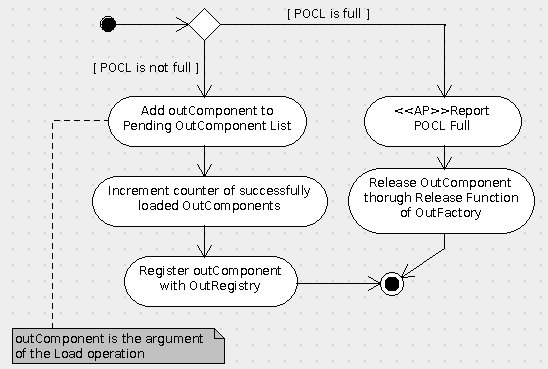
\includegraphics[scale=0.45,keepaspectratio=true]{OutManagerLoad.png}
 \caption{The OutManager Load Procedure}
 \label{fig:OutManagerLoad}
\end{figure}

The OutComponents loaded into the POCL must be fully configured (i.e. they must be in state CONFIGURED). It is the responsibility of the user of the OutManager to ensure that this constraint is complied with. Note that, since OutComponents are loaded into the OutManager by the OutLoader (see previous section), this constraint must be enforced by the host application when it loads an out-going command or report into the OutLoader. Violation of this constraint will result in an OutComponent permanently remaining in the POCL of the OutManager.

The OutManager maintains a counter of successfully loaded OutComponents. The counter is initialized to zero when the OutManager is reset.

The order in which the items in the POCL are processed by the OutManager is unspecified.

There is no mechanism to “unload” a pending OutComponent. The OutManager autonomously returns an OutComponent to the OutFactory when the OutComponent has been sent to its destination (i.e. when the OutComponent is in state TERMINATED) or when it has been aborted (i.e. when the OutComponent is in state ABORTED). 

\begin{figure}[h]
 \centering
 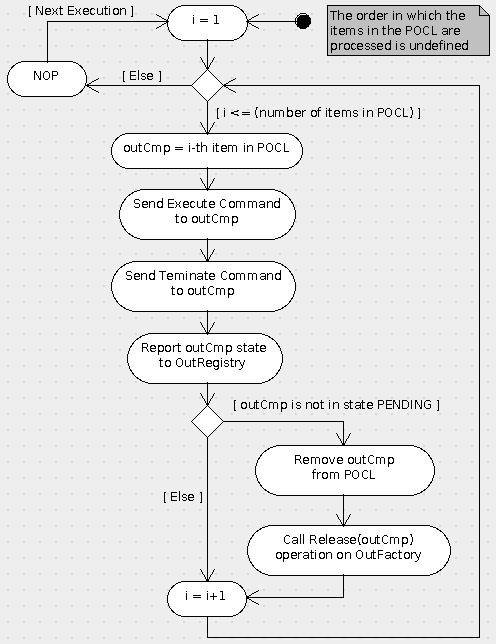
\includegraphics[scale=0.40,keepaspectratio=true]{OutManagerExecution.png}
 \caption{The OutManager Execution Procedure}
 \label{fig:OutManagerExecution}
\end{figure}

The OutManager component is defined as an extension of the Base Component of section \ref{sec:BaseCmp}. It uses the \textit{Execution Procedure} of the Base Component to process the pending commands. The OutManager component processes the pending commands by sending them an \texttt{Execute} command. After each \texttt{Execute} command, the state of the OutComponent is reported to the OutRegistry using the latter Update function (see figure \ref{fig:RegistryStartTrackingAndUpdate}). Commands which have been aborted or have been sent to their destination are removed from the POCL and are returned to the OutFactory. The \textit{Execution Procedure} of the OutManager is shown in figure \ref{fig:OutManagerExecution}.

Normally, the OutManager is embedded within a Real Time Container (see \cite{ref:fwprofile}) which is responsible for executing it. Thus, an application that is required to process out-going commands or reports at different levels of priority should use several OutManagers (one for each level of priority) and should allocate them to Real Time Containers with a matching priority.



The C2 Implementation implements the OutManager component in module \texttt{CrFwOutManager}. Its adaptation points are defined in \texttt{CrFwOutManagerUserPar.h} and only consist of the definition of the number of OutManagers in the application and of the size of their queue of pending OutComponents. 

As noted above, at CORDET Framework level, there is no requirement covering the order in which the OutComponents loaded into an OutManager are processed when the OutManager is executed. The C2 implementation, however, enforces the following ordering constraint. If OutComponents C1 to Cn are successfully loaded into an OutManager through through successive calls to its \texttt{Load} operation and if this sequence of \texttt{Load} operations is not interrupted by an execution of the OutManager, then, when the OutManager is executed next, the OutComponents C1 to Cn will be processed in the order in which they have been loaded.

%---------------------------------------------------------------------------------
\section{The OutRegistry Component}\label{sec:OutRegistry}
This component acts as a registry for out-going commands and reports (namely for commands or report which have been loaded into an OutManager).

The OutRegistry is defined as an extension of the Base Component of section \ref{sec:BaseCmp}. It has two functions: (a) it keeps track of an out-going command's or report's state; and (b) it stores the out-going command's or report's enable state.

The OutRegistry maintains a list of the last N commands or reports to have been loaded in all OutManagers in an application. The OutRegistry maintains the state of each such command or report. The command's or report's state in the OutRegistry can have one of the following values:
\begin{itemize}
\item PENDING: the command or report is waiting to be sent
\item ABORTED: the command or report was aborted because it was disabled when it was loaded
\item TERMINATED: the command or report has been passed to the OutStream
\end{itemize}
The value of N (the maximum number of items which can be tracked by the OutRegistry) is fixed and is an initialization parameter.

An OutComponent is first registered with the OutRegistry when it is loaded into the OutManager through the latter \texttt{Load} operation. Subsequently, the information in the OutRegistry is updated by the OutManagers every time a command or report is executed. Normally, a command's or report's state in the OutRegistry eventually becomes either ABORTED or TERMINATED. The only situation where this is not the case is\footnote{This exception could be avoided if the OutRegistry were notified of the reset of the OutManager. This is not done for reasons of simplicity and because it is expected that applications which reset an OutManager will normally also reset the OutRegistry.}: if an OutManager is reset, then the state of a command or report that was in state PENDING at the time the OutManager was reset will remain equal to PENDING.

The OutRegistry uses the identifier attribute (see sections \ref{sec:CmdAttributes} and \ref{sec:RepAttributes}) as the key through which the command or report state is stored.

\begin{figure}[h]
 \centering
 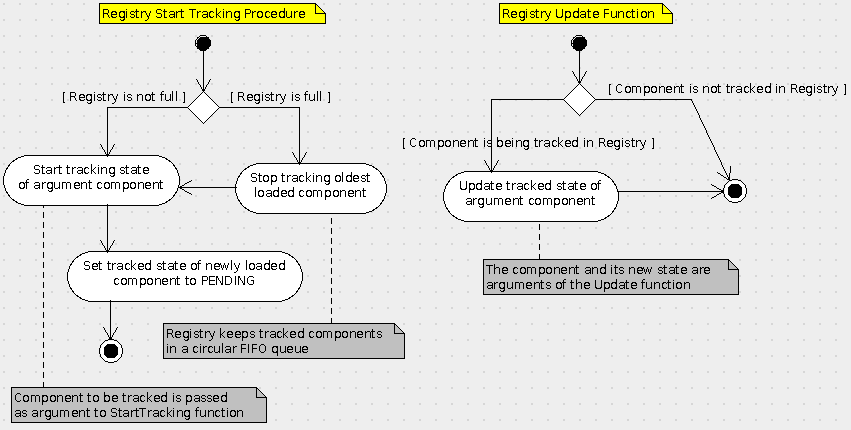
\includegraphics[scale=0.5,keepaspectratio=true]{RegistryStartTrackingAndUpdate.png}
 \caption{The Registry Start Tracking and Registry Update Procedures}
 \label{fig:RegistryStartTrackingAndUpdate}
\end{figure}

In order to perform the tasks described above, the OutRegistry offers two operations: \texttt{StartTracking} and \texttt{Update}. These operations run the procedures Registry Start Tracking and Registry Update shown in figure \ref{fig:RegistryStartTrackingAndUpdate}. Operation \texttt{StartTracking} is performed by the \texttt{Load} operation of an OutManager to register an OutComponent with the OutRegistry. Operation \texttt{Update} is performed by the \textit{Execution Procedure} of an OutManager to ask the OutRegistry to update its information about an OutComponent's state.

The OutRegistry stores the enable state of out-going commands and reports. The enable state of out-going command and reports can be controlled at three levels: 
\begin{itemize}
\item[(a)] At the level of the service type (all commands or reports of a certain type are disabled)
\item[(b)] At the level of the service sub-type (all commands or reports matching a certain [type, sub-type] pair are disabled)
\item[(c)] At the level of the discriminant (all commands or reports matching a certain [type, sub-type, discriminant] triplet are enabled or disabled)
\end{itemize}
The enable state of a particular command or report is derived from these three enable levels by running the \textit{Enable State Determination Procedure} of figure \ref{fig:EnableStateDetermination}.

The OutRegistry offers an API through which all three levels of enable state can be set and read. By default, all enable states are set to: “enabled”. The enable states are configuration parameters for the OutRegistry which are reset to: “enabled” every time the component is reset.

As discussed in section \ref{sec:OutComponent}, by default, the Enable Check of an out-going command or report determines whether the command or report is enabled or not by reading its enable status from the OutRegistry. 

\begin{figure}[H]
 \centering
 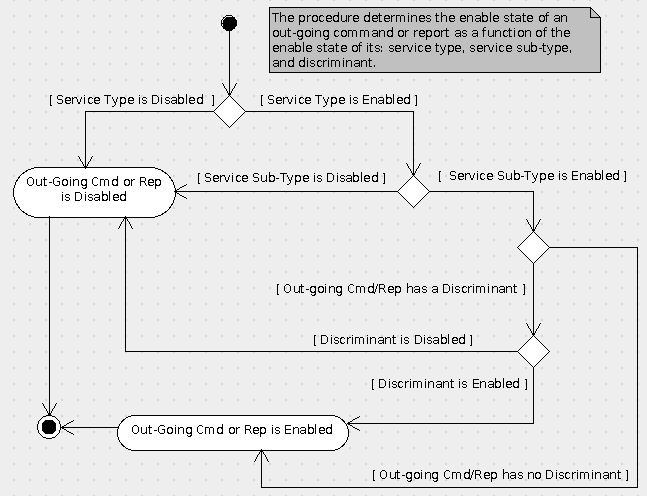
\includegraphics[scale=0.5,keepaspectratio=true]{EnableStateDetermination.png}
 \caption{The Enable State Determination Procedure}
 \label{fig:EnableStateDetermination}
\end{figure}



The C2 Implementation implements the OutRegistry component in module \texttt{CrFwOutRegistry}. Its adaptation points are defined in \texttt{CrFwOutRegistryUserPar.h} and include a list of all service types and sub-types supported by the application. The information in this header file must be consistent with the information in \texttt{CrFwOutFactoryUserPar.h}.

\clearpage
%=================================================================================
\section{The InLoader Component}\label{sec:InLoader}
The InLoader is responsible for retrieving incoming packets which become available at an InStream. 

The InLoader component is defined as an extension of the Base Component of section \ref{sec:BaseCmp}.  It overrides its \textit{Execution Procedure} with the procedure shown in figure \ref{fig:InLoaderExecution} (the \textit{InLoader Execution Procedure}). 

The InLoader should be executed when one or more packets have become available at the InStream. The logic of its execution procedure can be summarized as follows.
The procedure processes incoming packets one by one. A packet is retrieved from the InStream through the \texttt{GetPacket} operation. If the operation does not return any packet, then the procedure stops and waits for the next execution. If instead the \texttt{GetPacket} operation returns a fresh packet, the procedure extracts its destination. This is an adaptation point because it requires knowledge of the packet's layout. If the packet's destination is invalid (the destination validity check is another adaptation point), the procedure reports the fact and then attempts to retrieve the next packet from the InStream (or it holds until the next execution cycle if no more packets are available in the InStream).

If the packet destination is valid but is not the host application, then the packet is re-routed. This means that a re-routing destination is determined for the packet and the packet is forwarded to this re-routing destination. The re-routing destination can be either the eventual packet destination (if the host application has a direct link to the packet's destination) or it can be an intermediate destination. The packet is forwarded by directly loading it into the OutStream associated to the re-routing destination. The OutStream is retrieved through the OutStreamRegistry component of section \ref{sec:OutStream}. 

The determination of the re-routing destination depends on the connection topology of the system within which the application is embedded and is therefore an adaptation point. The re-routing information is a configuration-level information which can only be modified by resetting the InLoader.

\begin{figure}[h]
 \centering
 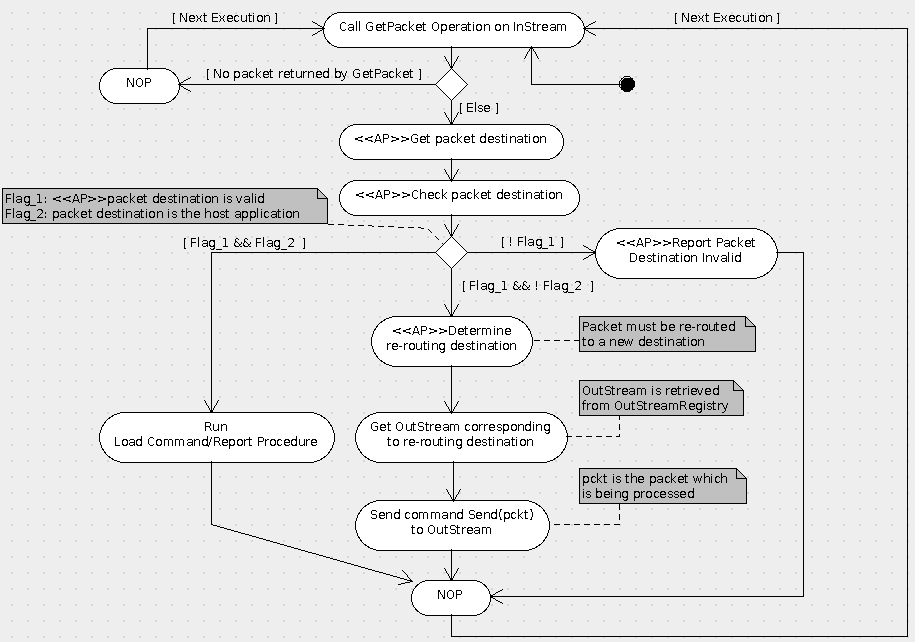
\includegraphics[scale=0.35,keepaspectratio=true]{InLoaderExecution.png}
 \caption{The InLoader Execution Procedure}
 \label{fig:InLoaderExecution}
\end{figure}

If the packet destination is the host application, then the incoming packet is processed by the \textit{Load Command/Report Procedure}. This procedures is shown as activity diagrams in figure \ref{fig:InLoaderLoadCommandReport}. Its logic can be summarized as follows.

The procedures begin by retrieving the command or report type from the packet. The type is given by the triplet: [service type, service sub-type, discriminant]. This is an adaptation point because it requires knowledge of the packet layout. If the packet type is not valid (i.e. if it is not supported by the host application), then the packet is rejected and the incoming command or report is deemed to have failed its Acceptance Check.

If the packet type is valid, it is used to retrieve an InCommand or InReport instance from the InFactory (it is recalled that the type determines whether the packet holds a command or a report). The InCommand or InReport instance is retrieved from the InFactory using its \texttt{Make} operation. If the creation of the InCommand or InReport instance fails, the packet is rejected and the incoming command or report is deemed to have failed its Acceptance Check.

If the creation of the InCommand or InReport instance succeeds, the packet is deserialized to configure the InCommand or InReport instance. After the deserialization has been completed, the InCommand or InReport is initialized and reset. The reset process is used as part of the acceptance check for the incoming command or report. If the information in the packet was syntactically correct and complete, then the initialization and reset operations succeed and the InCommand or InReport enters state CONFIGURED.

If the InCommand or InReport fails to enter its state CONFIGURED, it is rejected and the InCommand or InReport is deemed to have failed its Acceptance Check and is returned to the InFactory.

If the command or report is successfully configured, then it must be loaded into an InManager. For this purpose, the InLoader maintains a list of InManagers (the LIM or \textit{List of InManagers}). The size and content of this list are fixed and are defined when the InLoader is configured. The selection algorithm for the InManagers is an adaptation point. By default, the LIM has two entries and the InLoader selects the first item in the LIM for incoming InCommands and second item for incoming InReports. 
No facilities are provided for dynamically changing the set of InManagers. Changes in the set of InManagers can only be done by reconfiguring and then resetting the component.

The \texttt{Load} operation in the InManager may either succeed or fail (see section \ref{sec:InManager}). If it succeeds, the InCommand or InReport is deemed to have passed its Acceptance Check. 
  
If the \texttt{Load} operation in the InManager fails, the InCommand or InReport is deemed to have failed its Acceptance Check. This results in the InCommand or InReport component being returned to the InFactory.

Thus, in summary, an InCommand or InReport is deemed to have failed its Acceptance Check if any of the following conditions is satisfied:
\begin{fw_itemize}
\item The incoming packet holding the InCommand or InReport has an invalid type;
\item The InFactory fails to return a component to hold the InCommand or InReport encapsulated in the incoming packet;
\item The InCommand or InReport fails to enter state CONFIGURED;
\item The InCommand or InReport fails to be loaded into the InManager.
\end{fw_itemize}
In all other cases, the InCommand or InReport is regarded as having passed its Acceptance Check. 

Failure of the Acceptance Check is reported. The reporting of the failure is an adaptation point. The passing of the Acceptance Check has no consequences for an InReport whereas in the case of InCommands it may result in an Acceptance Successful Report being generated to the command's sender if this is required by the setting of the Acknowledge Level attribute of the InCommand (i.e. each InCommand carries information that determines whether its passing its Acceptance Check ought to be reported to the command sender, see section \ref{sec:CmdAttributes}). 

\begin{figure}[H]
 \centering
 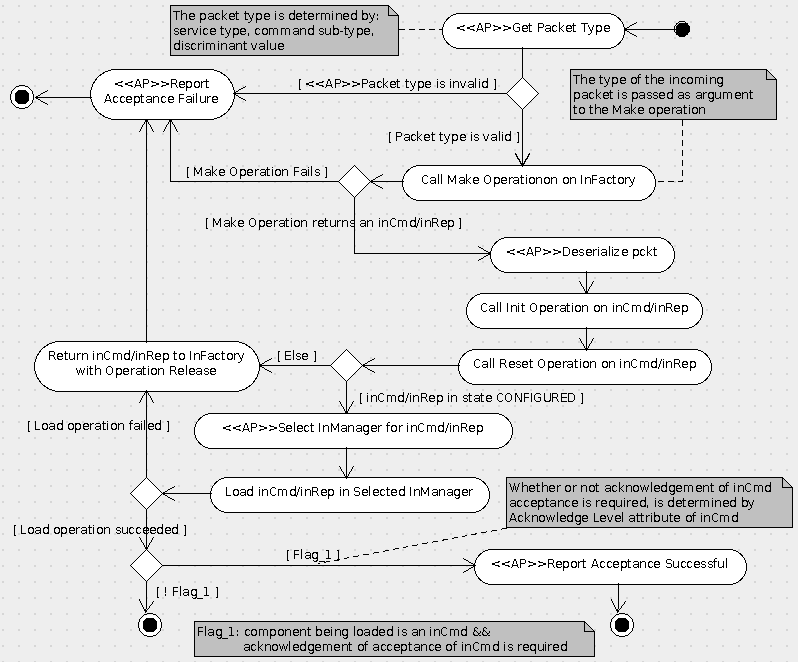
\includegraphics[scale=0.35,keepaspectratio=true]{InLoaderLoadCommandReport.png}
 \caption{The InLoader Load Command/Report Procedure}
 \label{fig:InLoaderLoadCommandReport}
\end{figure}



The C2 Implementation implements the InLoader component in module \texttt{CrFwInLoader}. Its adaptation points are defined in \texttt{CrFwInLoaderUserPar.h} but the following should be noted with respect to the implementation of the acceptance check. As discussed above, this check is split into four sub-checks. Sub-checks 1 and 2 and sub-check 4 are implemented at framework level. The third sub-check is instead application-specific. It is called the Validity Check (because it verifies the validity of the parameters of the incoming report or command) and is implemented by a user-provided function which must conform to the prototype of function pointers \texttt{CrFwInRepValidityCheck\_t} for incoming reports or \texttt{CrFwInCmdValidityCheck\_t} for incoming commands. The functions implementing the validity checks are defined in \texttt{CrFwInFactoryUserPar.h}.

The implementation of the validity check would typically include the check on the correctness of the InReport's or InCommand's CRC.

%=================================================================================
\section{The InCommand Component}\label{sec:InCommand}
The InCommand component encapsulates an incoming command in a provider application. This component enforces the generic behaviour that is common to all incoming commands irrespective of their type and it provides read-only access to a command's attributes. The InCommand component is an extension of the Base Component of section \ref{sec:BaseCmp}. 

Incoming commands must be accepted before they can be executed (see section \ref{sec:CmdLifecycle}). The acceptance check is implemented partly by the InLoader (see section \ref{sec:InLoader}) and partly by the initialization and configuration checks of the InCommand itself.

The behaviour of a command that has been accepted is modelled by the state machine shown in figure \ref{fig:InCommand} (the \textit{InCommand State Machine}). This state machine is embedded within the CONFIGURED state of the Base State Machine. 

\begin{figure}[h]
 \centering
 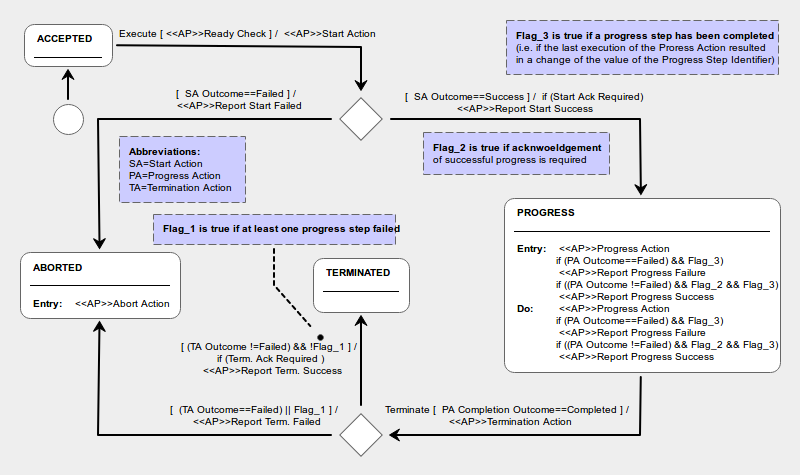
\includegraphics[scale=0.47,keepaspectratio=true]{InCommand.png}
 \caption{The InCommand State Machine}
 \label{fig:InCommand}
\end{figure}

When the state machine is started (i.e. when the command is accepted and the InCommand enters state CONFIGURED), it enters state ACCEPTED. In this state, the InCommand component waits for sequences of Execute and Terminate commands. The constraint that an InCommand component should be sent \texttt{Execute} and \texttt{Terminate} requests in sequence is enforced by the InManager which is responsible for controlling the execution of InCommands (see section \ref{sec:InManager}).

Execution of the InCommand state machine in state ACCEPTED causes it to perform the Ready Check. The Ready Check – like all other command checks and command actions – is an adaptation point.  

If the Ready Check is failed (i.e. if the Ready Check indicates that the command is not yet ready to start execution), the command remains in state ACCEPTED.

If the Ready Check is passed (i.e. if the Ready Check indicates that the command is ready to start execution), the command executes the Start Action and, depending on its outcome, it makes a transition either to state ABORTED or to state PROGRESS.  

In state PROGRESS, the command executes its Progress Action. If the completion outcome of the Progress Action is "not completed” (indicating that the command has not yet completed execution), the InCommand remains in state PROGRESS. If, instead, the completiong outcome of the Progress Action is “completed” (indicating that all progress steps have been executed), then the InCommand moves out of the PROGRESS state and executes its termination action. The outcome of the termination action determines whether the command enters TERMINATED (to indicate a nominal end of the command) or ABORTED (to indicate that either one or more of its execution steps have failed or that its termination action has failed).  

The Progress Action is responsible for updating the Progress Step Identifier. A change in the value of this identifier marks the end of a Progress Step. A Progress step is a set logically related execution steps which are executed in sequence.

If the command is neither terminated nor aborted in the first Execute-Terminate cycle, it will be sent further pairs of Execute-Terminate commands by its InManager and will repeat the behaviour described in the previous paragraphs.  

The InCommand component is responsible for generating acknowledge reports. The acknowledge reports are generated: at the end of the start action; during execution of the progress action; and at the end of the termination action. At the end of the start and termination actions, either a success or a failure acknowledge report is generated depending on the outcome of the action. During the execution of the progress action, failure reports are generated whenever an execution step fails whereas success reports are generated whenever a progress step has terminated successfully. Success reports are only generated if the corresponding acknowledge flag is set in the InCommand. 

The generation of the acknowledge reports is an adaptation point for the InCommand. Note that the acknowledge report for the command acceptance is generated by the InLoader component, see section \ref{sec:InLoader}.

The InCommand component provides visibility over all attributes of the command it encapsulates but only predefines dummy values for them. The set and value of the command attributes is therefore an adaptation point for the InCommand.



The C2 Implementation implements the InCommand component in module \texttt{CrFwInCmd}. Applications will normally have to extend this component to create their own InCommand components. Typically, for each application-specific command, application developers should provide one C module which defines the functions implementing the actions and checks for that command. An example of how this can be done is provided in module \texttt{CrFwInCmdSample1} which implements a sample command used in the Test Suite.

The adaption points for InCommands are defined in \texttt{CrFwInFactoryUserPar.h}. This header file in particular defines the kinds of InCommands to be supported by an application. Each kind of supported InCommand is defined in terms of its service type, command sub-type and discriminant value (if applicable). For each supported InCommand kind, the application developers must specify the pointers to the functions which implement the actions and checks for that command kind.


%=================================================================================
\section{The InReport Component}\label{sec:InReport}
The InReport component encapsulates an incoming report in a user application. This component enforces the generic behaviour that is common to all incoming reports irrespective of their type and it provides read-only access to a report's attributes.

The InReport component is an extension of the Base Component of section \ref{sec:BaseCmp}. Incoming reports must be accepted before they can be executed (see section \ref{sec:RepLifecycle}). The acceptance check is implemented partly by the InLoader (see section \ref{sec:InLoader}) and partly by the initialization and configuration checks of the InReport itself.

\begin{figure}[h]
 \centering
 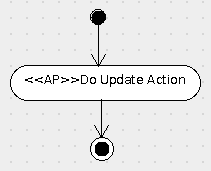
\includegraphics[scale=0.4,keepaspectratio=true]{InReportExecution.png}
 \caption{The InReport Execution Procedure}
 \label{fig:InReportExecution}
\end{figure}

The behaviour of a report that has been accepted is modelled by the procedure shown in figure \ref{fig:InReportExecution} (the \textit{InReport Execution Procedure}). This procedure is used as execution procedure for the InReport. The procedure simply executes the InReport's Update Action and then terminates. The Update Action is an adaptation point.

The InReport component provides visibility over all attributes of the reports it encapsulates but only predefines dummy values for them. The set and value of the report attributes is therefore an adaptation point for the InCommand.



The C2 Implementation implements the InReport component in module \texttt{CrFwInRep}. Applications will normally have to extend this component to create their own InReport components. Typically, for each application-specific command, application developers should provide one C module which defines the functions implementing the actions and checks for that report. An example of how this can be done is provided in module \texttt{CrFwInRepSample1} which implements a sample report used in the Test Suite.

The adaption points for InReports are defined in \texttt{CrFwInFactoryUserPar.h}. This header file in particular defines the kinds of InReports to be supported by an application. Each kind of supported InReport is defined in terms of its service type, command sub-type and discriminant value (if applicable). For each supported InReport kind, the application developers must specify the pointers to the functions which implement the actions and checks for that report kind.


%=================================================================================
\section{The InManager Component}\label{sec:InManager}
This component is responsible for maintaining a list of pending incoming commands and reports and for repeatedly executing them until they are either aborted or terminated.
The list of pending commands and reports is called the \textit{Pending Command/Report List} or PCRL. The PCRL has a fixed size which is defined when the InManager is initialized.
 
The InManager component offers a \texttt{Load} operation through which an InCommand or InReport can be added to the PCLR (see activity diagram in figure \ref{fig:InManagerLoad}). This operation is called by the InLoader of section \ref{sec:InLoader}. The \texttt{Load} operation may fail if the list is full. The order in which the items in the PCRL are processed is unspecified.

The \texttt{Load} operation registers the newly loaded InCommand or InReport with the InRegistry using the latter \texttt{StartTracking} operation (see section \ref{sec:InRegistry}). Henceforth, and as long as the InCommand or InReport remains loaded in the InManager, its state is tracked by the InRegistry. 

The InCommand and InReport components loaded into the PCRL must be fully configured (i.e. they must be in state CONFIGURED). Compliance with this constraint is guaranteed by the logic of the InLoader of section \ref{sec:InLoader}.

The InManager maintains a counter of successfully loaded InCommands or InReports. The counter is initialized to zero when the InManager is reset.

There is no mechanism to “unload” a pending command or report. The InManager autonomously returns a command or report component to the InFactory when the component has terminated execution. In the case of InCommands, execution can be terminated successfully (in which case the InCommand component is in state TERMINATED) or unsuccessfully (in which case the InCommand component is in state ABORTED). In the case of InReports, execution terminates after they are executed once. 

\begin{figure}[h]
 \centering
 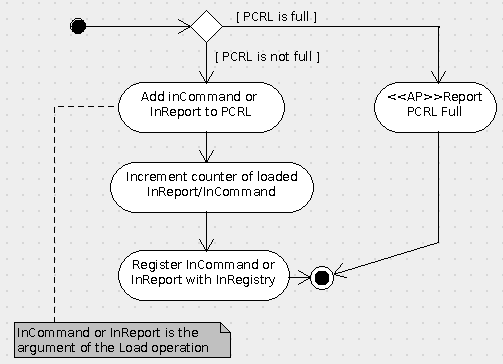
\includegraphics[scale=0.45,keepaspectratio=true]{InManagerLoad.png}
 \caption{The InManager Load Procedure}
 \label{fig:InManagerLoad}
\end{figure}

The InManager component is defined as an extension of the Base Component of section \ref{sec:BaseCmp}. It uses the \textit{Execution Procedure} of the Base Component to process the pending commands and reports. The InManager component processes the pending commands and reports by sending them an \texttt{Execute} command and a \texttt{Terminate} command (note that the \texttt{Terminate} command has no effect on an InReport).

After the \texttt{Terminate} command, the state of the InCommand or InReport is reported to the InRegistry using the latter \texttt{Update} operation (see section \ref{sec:InRegistry}). InCommands which have terminated execution are removed from the PCRL and are returned to the InFactory. InReports are returned to the InFactory after their first execution. The \textit{Execution Procedure} of the InManager is shown in figure \ref{fig:InManagerExecution}.

Normally, the InManager is embedded within a Real Time Container (see \cite{ref:fwprofile}) which is responsible for executing it. Thus, an application that is required to process commands and reports at different levels of priority should use several InManagers (one for each level of priority) and should allocate them to Real Time Containers with a matching priority.

\begin{figure}[H]
 \centering
 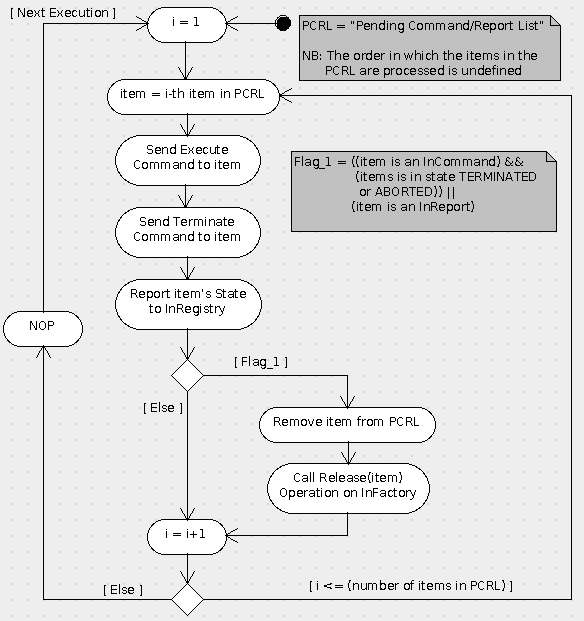
\includegraphics[scale=0.35,keepaspectratio=true]{InManagerExecution.png}
 \caption{The InManager Execution Procedure}
 \label{fig:InManagerExecution}
\end{figure}



The C2 Implementation implements the InManager component in module \texttt{CrFwInManager}. Its adaptation points are defined in \texttt{CrFwInManagerUserPar.h}.

As noted above, at CORDET Framework level, there is no requirement covering the order in which the InReports or InCommands loaded into an InManager are processed when the InManager is executed. The C2 implementation, however, enforces the following ordering constraint. If InReports/InCommands C1 to Cn are successfully loaded into an InManager through successive calls to its \texttt{Load} operation and if this sequence of \texttt{Load} operations is not interrupted by an execution of the InManager, then, when the InManager is executed next, the InReports/InCommands C1 to Cn will be processed in the order in which they have been loaded.

%=================================================================================
\section{The InRegistry Component}\label{sec:InRegistry}
This component acts as a registry for incoming commands and reports (namely for commands and reports which have been loaded into an InManager).

The function of the InRegistry is to keep track of an incoming command state or of an incoming report state.

The InRegistry maintains a list of the last N commands or report to have been loaded in one of the InManagers in an application. For each such command or report, the InRegistry maintains a record of its state. The command or report state in the InRegistry can have one of the following values:
\begin{itemize}
\item PENDING: the command or report is executing
\item ABORTED: the command was aborted during its execution by the InManager
\item TERMINATED: the command or report has successfully completed its execution
\end{itemize}
Note that state ABORTED only applies to incoming commands.

The value of N (the maximum number of commands or reports which are tracked by the InRegistry) is fixed and is an initialization parameter.

An InCommand or InReport is first registered with the InRegistry when it is loaded into the InManager through the latter \texttt{Load} operation. Subsequently,the information in the InRegistry is updated by an InManager every time a command or report is executed. Normally, a command or report state in the InRegistry eventually becomes either ABORTED or TERMINATED. The only situation where this is not the case is when an InManager is reset. In that case, commands and reports which were pending in the InManager at the time it was reset may never terminate \footnote{This is due to the fact that, when the InManager is reset, its list of pending commands and reports is cleared. It might be argued that the InRegistry should be notified of this fact so as to give it a chance to update the information it holds about commands which are currently in state PENDING. This is not done for reasons of simplicity and because it is expected that applications which reset an InManager will also  reset the InRegistry.}.

The InRegistry uses the command identifier attribute (see section \ref{sec:CmdAttributes}) as the key through which the command state is classified.

In order to perform the tasks described above, the InRegistry offers two operations: \texttt{StartTracking} and \texttt{Update}. These operations implement the same behaviour as the operations of the same name in the OutRegistry, namely they run, respectively, the Registry Start Tracking Procedure and the Registry Update Procedure (see figure \ref{fig:RegistryStartTrackingAndUpdate}). Operation \texttt{StartTracking} is called by the \texttt{Load} operation of an InManager to register an InCommand or InReport with the InRegistry. Operation \texttt{Update} is called by the \textit{Execution Procedure} of an InManager to ask the InRegistry to update its information about an InCommand or InReport state.



The C2 Implementation implements the InRegistry component in module \texttt{CrFwInRegistry}. Its adaptation points are defined in \texttt{CrFwInRegistryUserPar.h}.


%=============================================================================================
\section{Memory Management}\label{sec:MemMng}

The C2 Implementation uses memory for its data and its code. Memory for data is allocated either globally, or on the stack, or on the heap.

Globally allocated variables are defined in the header files of the framework modules as \texttt{static} variables. They are therefore not visible outside the module where they are defined and used.

Local function variables are allocated on the stack. The amount of stack memory used for this purpose is limited as in most cases only a handful of pointers and variables of primite type are used.

Allocation on the heap is done through the \texttt{malloc} function and is limited to the following cases:

\begin{itemize}
\item Allocation of memory for components subject to early instantiation (see section \ref{sec:CmpInst}). This allocation is done in factory functions which are called during the application start-up phase. The memory thus allocated is never released.
\item Allocation of memory for packet queues in module \texttt{CrFwPcktQueue}. This operation is performed as part of the initialization action of the InStream and OutStream components. The memory thus allocated is released when the InStream or OutStream are shutdown.
\item Allocation of memory for the data structure holding the enable status of commands and reports in the \texttt{CrFwOutRegistry} module. This operation is performed as part of the initialization action of the OutRegistry component. The memory thus allocated is released when the OutRegistry is shutdown.
\item Allocation of memory for the Pending OutComponent List (POCL) in the \texttt{CrFwOutManager} module. This operation is performed as part of the initialization action of the OutManager component. The memory thus allocated is released when the OutManager is shutdown.
\item Allocation of memory for the Pending Command/Report List (PCRL) in the \texttt{CrFwInManager} module. This operation is performed as part of the initialization action of the InManager component. The memory thus allocated is released when the InManager is shutdown.
\item Allocation of memory for the arrays holding the sequence counters for the destination/source groups associated to an InStream in the \texttt{CrFwInStream} module. This operation is performed as part of the initialization action of the InStream component. The memory thus allocated is released when the InStream is shutdown.
\item Allocation of memory for the arrays holding the sequence counters for the destination/source groups associated to an OutStream in the \texttt{CrFwOutStream} module. This operation is performed as part of the initialization action of the OutStream component. The memory thus allocated is released when the OutStream is shutdown.
\end{itemize}

Thus, in all cases, memory allocation is done as part of the initialization of the application of a component. During normal operation (i.e. when the application is in state NORMAL, see section \ref{sec:AppStartUp}), no allocation of memory on the heap is ever performed.

The C2 Implementation does not handle the case where the call to \texttt{malloc} fails.  This is acceptable because the \texttt{malloc} calls are only performed during application or component initialization and hence the number of calls and the amount of memory they claim can be determined statically. It is therefore possible for the application developer to ensure that sufficient memory is available and to guarantee by design that no \texttt{malloc} failures can occur.

Release of heap memory is done through calls to the \texttt{free} function. This is exclusively done in the shutdown operations of the components which had allocated memory as part of their initialization. 

Thus, in summary, dynamic memory allocation on the heap is only done as part of the instantiation of the framework component and, in some cases, of their initialization. The memory which is allocated on the heap during early instantiation of components is never released (because components instantiated early are not intended to be ever destroyed). The memory which is allocated as part of component initialization is released when the components are shutdown.

For components which allocate memory from the heap as part of their initialization (OutRegistry, InManager, OutManager, InStream and OutStream) two paths to a memory leak are possible:

\begin{itemize}
\item A component is stopped after it has been initialized and then it is initialized again
\item A component is initialized more than once without being shut down
\end{itemize}

Responsibility for avoiding the first kind of memory leak rests with the user who should avoid stopping a component (a shutdown should be performed instead). The second kind of memory leak is not possible in the case of the OutRegistry, InManager and OutManager components because their initialization action always returns an outcome of "success". This implies that the initialization action can only be executed once before the component is shut down (see figure \ref{fig:BaseSM}). The InStream and OutStream, too, have default initialization action which always returns an outcome of "success" (see functions \texttt{CrFwInStreamDefInitAction} and \texttt{CrFwOutStreamDefInitAction}) but these functions can be extended or overridden by a user. In this case, it is up to the user to ensure the proper management of memory allocation. 

Late instantiation of components does not require any allocation of memory from the heap because the factory components which are responsible for the instantiation manage pools of pre-allocated memory which is allocated globally during application initialization. This is discussed at greater length in the next section.

Applications which do not wish to link to the standard \texttt{malloc} and \texttt{free} functions can: (a) define their own \texttt{malloc} function to, for instance, allocate memory sequentially from a pre-allocated array of fixed size, and (b) avoid ever shutting down a component thus avoiding calls to \texttt{free}. 

The C2 Implementation is designed to minimize code memory footprint. The exact memory requirements for its code depend on the choice of compiler and linker but will typically be of the order of several kBytes. As an example, table \ref{tab:memFootprint} reports the memory requirements for the files which implement the framework components. 

The figures in the table have been obtained with the gcc compiler configured to minimize memory occupation. The data in the table were derived from the linker map. They correspond to the memory of type \texttt{.text} (i.e. the code segment containing executable instructions) allocated to each module. The measurements were made on the beta release 0.1.0 of the C2 Implementation in the following environment:

\begin{itemize}
\item{compiler}: gcc version 4.6.3 (Ubuntu/Linaro 4.6.3-1ubuntu5)
\item{target}: i686-linux-gnu
\item{OS}: Linux ubuntu 12.04 (32 bits)
\item{compiler options}: -Os -Wall -c -fmessage-length=0
\item{linker options}: -Wl,-Map=memory.map
\end{itemize}

\begin{longtable}{|p{2.7cm}|p{2.7cm}|p{4.7cm}|}
\caption{Code Memory Footprint for C2 Implementation Modules} \label{tab:memFootprint}\\
\rowcolor{light-gray}
\textbf{Module} & \textbf{Memory Size} & \textbf{Header File} \\
\hline\hline
\endfirsthead
\rowcolor{light-gray}
\textbf{Module} & \textbf{Memory Size} & \textbf{Header File} \\
\hline\hline
\endhead
\emph{Base Component} & 1411 bytes & \texttt{CrFwBaseCmp.h}, \texttt{CrFwDummyExecProc}, \texttt{CrFwInitProc}, \texttt{CrFwResetProc} \\
\hline
\emph{InCommand} & 1680 bytes & \texttt{CrFwInCmd.h} \\
\hline
\emph{InRegistry} & 545 bytes & \texttt{CrFwInRegistry.h} \\
\hline
\emph{InManager} & 1208 bytes & \texttt{CrFwInManager.h} \\
\hline
\emph{InReport} & 292 bytes & \texttt{CrFwInRep.h}, \texttt{CrFwInRepExecProc.h} \\
\hline
\emph{InLoader} & 919 bytes & \texttt{CrFwInLoader.h} \\
\hline
\emph{InFactory} & 2188 bytes & \texttt{CrFwInFactory.h} \\
\hline
\emph{InStream} & 1416 bytes & \texttt{CrFwInStream.h} \\
\hline
\emph{OutComponent} & 1089 bytes & \texttt{CrFwOutCmp.h} \\
\hline
\emph{OutFactory} & 1397 bytes & \texttt{CrFwOutFactory.h} \\
\hline
\emph{OutLoader} & 357 bytes & \texttt{CrFwOutLoader.h} \\
\hline
\emph{OutManager} & 1066 bytes & \texttt{CrFwOutManager.h} \\
\hline
\emph{OutRegistry} & 1415 bytes & \texttt{CrFwOutRegistry.h} \\
\hline
\emph{OutStream} & 1373 bytes & \texttt{CrFwOutStream.h} \\
\hline
\emph{Packet Queue} & 499 bytes & \texttt{CrFwPcktQueue.h} \\
\hline
\textbf{Total} & 16855 bytes &  \\
\hline
\end{longtable}

% --------------------------------------------------------------------------------
\subsection{Components with Late Instantiation}

The late instantiation mechanism (see section \ref{sec:CmpInst}) is used for the components which encapsulate commands and reports (namely the InReport, InCommand and OutComponent components). As commands and reports are sent and received by an application during its normal operation, the components which encapsulate them must also be created and destroyed during normal operation ("late component instantiation"). The creation and destruction of these components is done through the \texttt{Make} and \texttt{Release} functions provided by the InFactory and OutFactory components.

Each command or report component encapsulates a packet which holds the sequence of bytes which represents the packet at middleware level (see \ref{sec:MwLayer}). Packets, too, must be created and destroyed during normal operation through calls to the \texttt{Make} and \texttt{Release} functions of \texttt{CrFwPckt.h}.

There are two functional chains through which a command or report component is created, used and then destroyed. The first chain arises when a command or report is received by an application. Figure \ref{fig:InCmpMakeRelChain} shows this chain as an activity diagram. Note that all activities in the diagrams are performed by framework components. Application components are therefore not involved in the processing of incoming commands and reports.

Similarly, figure \ref{fig:OutCmpMakeRelChain} shows the functional chain through which an out-going command or report is processed. Activities in the yellow bubbles are executed by the application; the other activities are instead executed by the framework components. 

The point of figures \ref{fig:InCmpMakeRelChain} and \ref{fig:OutCmpMakeRelChain} is to show that, under nominal conditions, command and report components which are created during normal operation through a call to a \texttt{Make} function are always eventually released through a call to a \texttt{Release} function. The only situations where this is \textbf{not} the case are:

\begin{itemize}
\item The processing of an out-going command or report component by the OutManager never completes (i.e. the out-going command or report neither terminates nor is aborted). The out-going command or report remains permanently loaded in the OutManager and its memory is consequently never released. 
\item The processing of an incoming command or report component by the InManager never completes (i.e. the incoming command or report neither terminates nor is aborted). The incoming command or report remains permanently loaded in the InManager and its memory is consequently nver released. 
\item The application requests and obtains an OutComponent from the OutFactory but never completes its configuration and therefore never loads the OutComponent in the OutLoader. The OutComponent remains permanently with the application and is therefore never released.
\item A component involved in the processing of commands or reports is reset or shutdown at a time when command or report components are pending.
\end{itemize}

The first two cases arise as a result of erroneous definitions of a command or report (for instance, by having a command whose Start Check never allows command execution to be started). The last two cases arise because of an error in the application. In all other cases, absence of memory leaks is guaranteed by the framework design.

\begin{figure}[h]
 \centering
 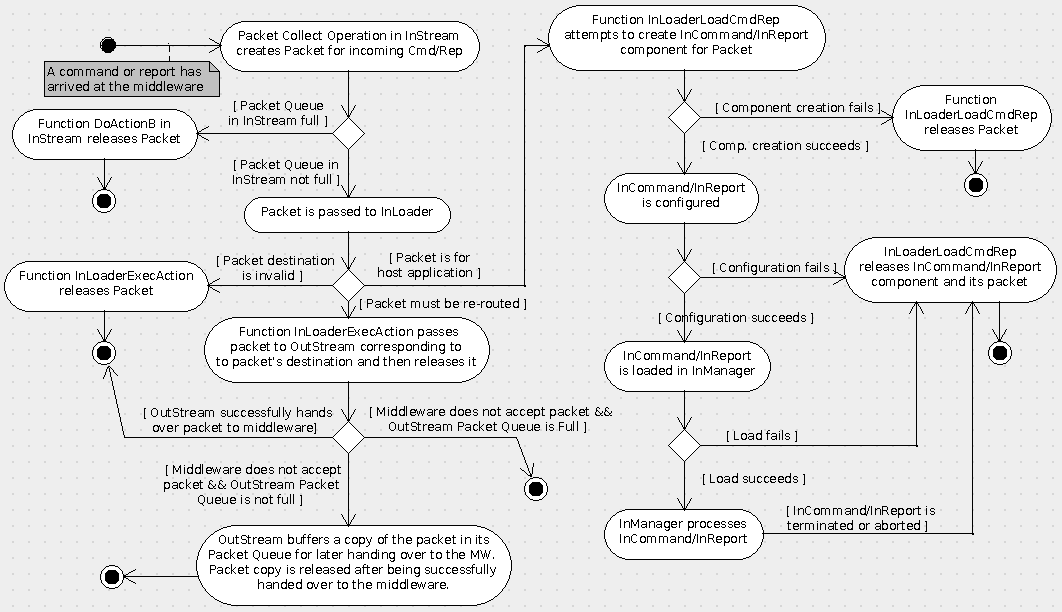
\includegraphics[scale=0.37,keepaspectratio=true]{InCmpMakeRelChain.png}
 \caption{Processing Chain for an Incoming Command or Report}
 \label{fig:InCmpMakeRelChain}
\end{figure}

\begin{figure}[H]
 \centering
 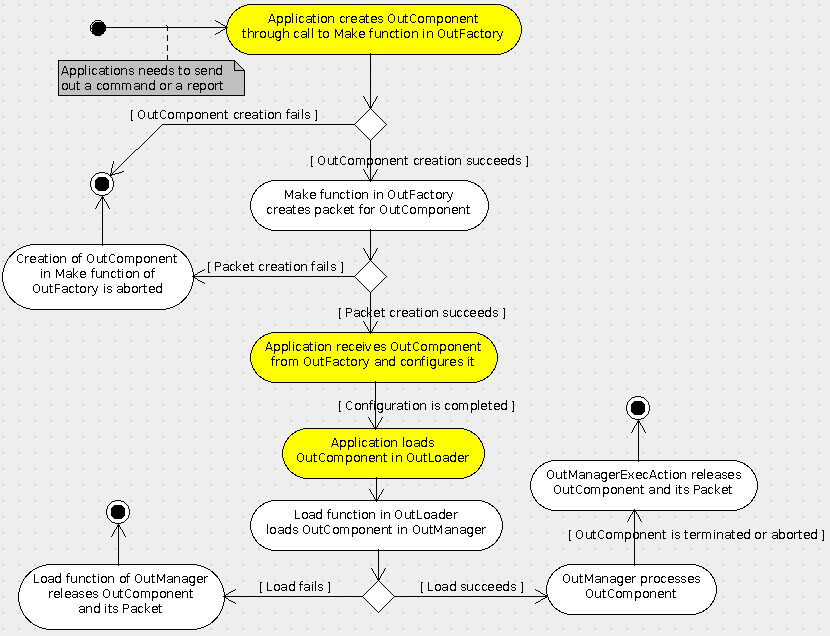
\includegraphics[scale=0.45,keepaspectratio=true]{OutCmpMakeRelChain.png}
 \caption{Processing Chain for an Out-Going Command or Report}
 \label{fig:OutCmpMakeRelChain}
\end{figure}

\clearpage
%=============================================================================================
\section{Real Time Issues}\label{sec:RTIssues}
The domain of the CORDET Framework are embedded control applications. These applications are often subject to real-time constraints. This section considers some issues which related to the usage of the C2 Implementation in a real-time environment.

% --------------------------------------------------------------------------------
\subsection{Scheduling of Framework Components}
The C2 Implementation does not define any "active components": none of its components create or manage threads of execution. All of its components expect to be called from outside. The entry points for an external scheduler are listed in table \ref{tab:EntryPoints}. The order in which they are listed is approximately the order in which they will typically be called but no specific ordering sequence is mandated by the C2 Implementation. 

Often a cyclical scheduling approach will be used for the entry points listed in the table (with the possible exceptions of the first and the last entries which might be attached to signals or interrupts from the middleware). Multiple cycles with different periods might also be used where the high frequency cycles are used to process high-priority commands/reports and the low frequency cycles are used to process low-priority commands/reports.

One option for implementing the link between the components listed in the table and a scheduler is to use the "Real-Time Containers" of reference [FW-SP] (a C-language implementation is available from reference [FW-SP]).

\begin{longtable}{|>{\centering\arraybackslash}m{0.3cm}|>{\raggedright}p{4.0cm}|p{8.5cm}|}
\caption{Entry Points for Scheduler} \label{tab:EntryPoints}\\
\hline
\rowcolor{light-gray}
\textbf{N} & \textbf{Entry Point} & \textbf{Description} \\
\hline\hline
\endfirsthead
\rowcolor{light-gray}
\textbf{N} & \textbf{Entry Point} & \textbf{Description} \\
\hline\hline
\endhead
1 & Send Command \texttt{CrFwInStreamPcktAvail} to the InStreams
& Command must be sent when a packet becomes available at the Middleware Interface or else it can be sent periodically (polling).
\\\hline
2 & Execute InLoader
& Causes incoming packets collected by the InStreams to be de-serialized and transformed into components which are then loaded into the InManagers. 
\\\hline
3 & Execute InManagers
& Causes incoming reports and commands which are pending in the InManagers to be processed. 
\\\hline
4 & Deleted & Deleted.
\\\hline
5 & Execute OutManagers
& Causes out-going reports and commands which are pending in the OutManagers to be processed.
\\\hline
6 & Send Command \texttt{CrFwOutStream-
ConnectionAvail} to the OutStreams
& Command must be sent when the out-going Middleware connection for an OutStream has become available or else it can be sent periodically (polling).
\\\hline
\end{longtable}

% --------------------------------------------------------------------------------
\subsubsection{Concurrency}
The C2 Implementation uses global variables (see section \ref{sec:MemMng}) but does not implement any mechanisms to ensure access in mutual exclusion to these variables. It is therefore not suited for use in a concurrent environment. It is the responsibility of the user to ensure that its components are accessed mutual exclusion.

% --------------------------------------------------------------------------------
\subsubsection{Recursion}
None of the functions defined by the C2 Implementation are recursive. Recursion is used to a limited extent in the libraries which implement the state machine and procedure model used by the C2 Implementation (see section \ref{sec:SmAndPrModel}). However, the depth of recursion is limited to 2 (because the depth of recursion is equal to the number of levels of embedding of state machines and, in the C2 Implementation, only one level of state machine embedding is used).  


%=============================================================================================
\section{Error Handling}\label{sec:ErrHandling}

In general, the C2 Implementation is intended for applications whose design is validated and whose implementation is verified. They therefore only handle errors which arise as a result of the application receiving at run-time inputs from outside which are illegal (i.e. inputs which are outside the boundaries specified for the application). 

The inputs for the C2 Implementation are the incoming commands and reports. These may be "illegal" either because their content is illegal or because the time pattern with which they are sent is illegal. The resulting error situations are specified by the CORDET Framework in reference [CR-SP]. The CORDET Components handle these errors by reporting them through the \textit{CrFwRepErr.h} interface. This interface is one of the adaptation points of the framework and must be implemented by applications according to their needs. 

A typical implementation of the error reporting interface could be as follows. The user defines a service to report errors and implements the \textit{CrFwRepErr.h} interface to generate reports belonging to that service and carrying a description of the error. Different report sub-types can be defined to represent different levels of severity. An example of this approach is the so-called "Event Reporting Service" of the PUS (see reference [PS-SP]). The range of errors handled through this mechanism is defined by the enumerated type \texttt{CrFwRepErrCode\_t}.

In addition to handling these exogenous error situations, the C2 Implementation also handles a limited number of "Applicaton Errors". Application errors arise as a result of a design or implementation error in the application itself. The situations which are handled by the C2 Implementation are those which satisfy the following constraints:

\begin{itemize}
\item The error situation arises when a framework function has been called by the application code with an illegal parameter value or in an illegal context and execution of the function with that value or in that context would cause an internal framework data structure to be corrupted.
\item The check for the error can be implemented with a minimal impact on memory and CPU consumption.
\end{itemize}

Thus, the objective of the handling of application errors is to shield a component's internal data structures. Note that no handling of errors is implemented when the incorrect calling parameters or calling context of a function would be harmful for the caller. 

Application errors are handled as follows. The function where the error is detected sets an \textit{application error code} and then returns. Nominally, the application error code should be equal to: \texttt{crNoAppErr}. If the application error code has a different value, then an application error has been encountered. If multiple errors have been encountered, the application error code reflects the most recent error.

If the application error code has a non-nominal value, the behaviour of the framework component is undefined and will normally be erroneous. The application error code can be accessed through function \texttt{CrFwGetAppErrCode}. 

The range of application error codes is defined by the enumerated type \texttt{CrFwAppErrCode\_t}.

%=============================================================================================
\section{Framework Instantiation Process}\label{sec:FwInstantiation}
The Framework Instantiation Process is the process through which the components provided by the framework are used to build an application within the framework domain. This section describes the steps required to instantiate the C2 Implementation of the CORDET Framework.

Two major steps are recognized in the instantiation process: 

\begin{enumerate}
\item[S1] Application Specification
\item[S2] Application Implementation
\end{enumerate}

Step S1 consists in casting (part of) the requirements of the target applications in terms of the services it provides to and requires from other entities in the system wihin which it is embedded. Step S2 consists in customizing the framework components to support the services defined in step S1. 

The table in the next page breaks up steps S1 and S2 into sub-steps. To each S1 sub-step, an S2 sub-step is associated (because each specification activity has an implementation-level counterpart). 

After all activities listed in the table have been performed, the application developer should have: (a) a complete specification of the framework-dependent part of his application and (b) a close-out for all adaptation points offered by the framework. The latter means that the framework components are ready for deployment in the target application. 

If the guidelines of section \ref{sec:fwSrcCode} are followed, the software of the instantiated framework will be organized as follows:

\begin{enumerate}
\item One directory (normally called \texttt{CrFramework}) holding the invariant part of the framework software. This directory can be a copy of the \texttt{CrFramework} in the Delivery File (see section \ref{sec:fwSrcCode}).
\item One directory (normally called \texttt{FwProfile}) holding the code implementing the state machine and procedure behaviour. This directory can be a copy of the \texttt{FwProfile} in the Delivery File (see section \ref{sec:fwSrcCode}).
\item One directory (normally called \texttt{CrConfig$\langle Name \rangle$} where "\texttt{Name}" is the name of the target application) holding the adaptable part of the framework software customized for the target application. This directory may be obtained by taking the \texttt{Config} directory in the Delivery File (\texttt{CrConfigTestSuite}) and then modifying its content as specified in the implementation steps.
\item One directory holding the application-specific software.
\end{enumerate}

In general, it is the responsibility of the user to ensure that the configuration information provided during the instantiation process is complete and consistent. A full check of completeness and consistency is not possible. However, the C2 Implementation offers module \texttt{CrFwAux} which implements a partial consistency check for the information in the \texttt{*UserPar} header files. Application developers should use this configuration check in the initial phase and can then remove it from their executable once confidence has been achieved that the configuration data are correct and complete.


\begin{landscape}

\pnpcsvtable{|>{\centering\arraybackslash}m{0.4cm}|>{\raggedright}p{2.0cm}|p{8.0cm}|p{9.0cm}|}{Framework Instantiation Specification and Implementation Steps}{tab:FwInstSteps}{\textbf{N} & \textbf{Step Name} & \textbf{Specification Sub-Step} & \textbf{Implementation Sub-Step}}{InstantiationProcess.csv}{\ID & \Title & \SpecificationStep & \ImplementationStep}

\end{landscape}


%===========================================================================
\section{Demo Application}\label{sec:DemoApp}
This section has been deleted.



\appendix
%===========================================================================
\section{Adaptation Points}\label{sec:AdaptationPoints}
The adaptation model of the C2 Implementation is described in section \ref{sec:AdaptationModel}. This appendix lists the adaptation points offered by the framework in table \ref{tab:AP}. The table is organized as follows:

\begin{itemize}
\item The left-most column in the table gives the identifier of the adaptation point. \item The middle column briefly describes the adaptation point.
\item The right-most column describes the location in the delivery file directory \texttt{/cr/src/CrConfigTestSuite} where the adaptation point is implemented.
\end{itemize}

With reference to the last point, it is recalled that all adaptation points are implemented as either \texttt{\#define} constants or \texttt{typedef} definitions in C header files in directory \texttt{/cr/src/CrConfigTestSuite} or as C body files in this same directory implementing framework interfaces.

Table \ref{tab:AP} only provides a summary view of the adaptation points. Their detailed definition is contained in the doxygen documentation of the files in the configuration directory \texttt{/cr/src/CrConfigTestSuite}.  

\begin{landscape}

\pnpcsvtable[filter not equal={\CTwoCat}{0}]{|l|p{7.2cm}|p{10.4cm}|}{C2 Implementation Adaptation Points}{tab:AP}{\textbf{AP ID} & \textbf{Adaptation Point} & \textbf{Implementation}}{../cordetfw/CordetFwAP.csv}{\CTwoCat-\CTwoId & \AP & \CTwoImpl}

\end{landscape}




\end{document}          

